
\documentclass[11pt,a4paper]{report} 
\renewcommand{\baselinestretch}{1.15} 
\usepackage[a4paper, total={6in, 8in}]{geometry}
\usepackage[hidelinks]{hyperref}
\usepackage[utf8]{inputenc}
\usepackage[affil-it]{authblk}
\usepackage[english]{babel}
\usepackage{polski}
\usepackage{siunitx}
\usepackage[export]{adjustbox}
\usepackage{graphicx, wrapfig}
\usepackage{tabularx}
\usepackage{amsmath}
\usepackage{fancyhdr}
\setlength{\headheight}{26pt}

\usepackage{amsfonts}
\usepackage{amssymb}
\usepackage{amsmath}
\usepackage{mathrsfs}
\usepackage[dvipsnames]{xcolor}
\usepackage{subfigure}
\usepackage[super]{nth}
\usepackage{indentfirst}
\usepackage{algorithm,algorithmic}
\usepackage{enumerate}
\usepackage[toc,page]{appendix}
\usepackage{amsthm}
\usepackage{textgreek}
\usepackage{upgreek}
\usepackage[siunitx,americaninductors]{circuitikz}
\usepackage{schemabloc}
\usetikzlibrary{circuits}
\usepackage{tikz, pgfplots}
\pgfplotsset{compat=1.15}
\usetikzlibrary{shapes,arrows,spy}
\usepackage{verbatim}
\usepackage[font=small,labelfont=bf]{caption}
\usepackage{array}
\newcolumntype{L}{>{\centering\arraybackslash}m{3cm}}
\usepackage{multirow}
\usepackage{paralist}
\usepackage{setspace}
\usepgfplotslibrary{polar}

\newcommand{\vect}[1]{\textbf{#1}}
\pagenumbering{Roman}

\begin{document}

% TITLE PAGE

\clearpage\thispagestyle{empty}
\begin{tabular}{m{2.15cm} m{8.0cm} m{3.2cm}}
        
\includegraphics[width=2.15cm]{title_pages/school_logos/pl_logo2.jpg} 
        &
        \begin{tabular}{c}
            \LARGE
             Lodz University of Technology\vspace{0.25cm}\\
             
             \Large
             Faculty of Mechanical Engineering\vspace{0.25cm}\\
             \Large
             Institute of Turbomachinery
        \end{tabular}
        & 
        
\includegraphics[width=3.2cm]{title_pages/school_logos/PL_logo1.png}
\end{tabular}

\vspace{1.0cm}
\begin{flushleft}
\LARGE
inż. Michał Wilczek
\\
\Large
Index no: 220242
\end{flushleft}

\begin{center}
    \vspace*{1cm}
    \LARGE
    \text{Master thesis}
    \Large
    \text{in}
    
    \text{Advanced Mechanical Engineering}
    \vspace{2.0cm}
   
   \LARGE
    \textbf{Heat Propagation Modelling in Superconducting Magnets based on Quench Velocity}
    \vspace{1.5cm}

    \text{Lodz University of Technology Supervisor}
    
    \text{dr hab. inż. Artur Gutkowski}
    \vspace{1.0cm}
   
    \text{CERN Supervisor}
    
    \text{Michał Maciejewski, PhD}
    \vspace{1.0cm}
            
    \text{Łódź, February 2020}
\end{center}
\newpage


\clearpage\thispagestyle{empty}
\chapter*{Abstract}
\thispagestyle{empty}

In this thesis, an electro-thermal multidimensional model is constructed in ANSYS APDL to simulate a discharge of the skew quadrupole being one of the high-order corrector magnets for the High-Luminosity LHC project. The analysis takes into consideration longitudinal and turn-to-turn quench propagation. The model is validated against available measurements of current and resistive voltage obtained during the discharge of the magnet. 

The quench propagation in superconducting magnets is a challenging task from the simulation point of view including multi-physics, multi-rate, multi-domain, and multi-scale problems. One has to take into consideration high material non-linearities being a function of temperature and, in some cases, magnetic field. 

A possibility of conducting the quench studies in ANSYS APDL is verified first. The models simulating a 1D quench propagation are prepared in ANSYS and compared with STEAM-BBQ being a tool for quench simulations implemented in COMSOL and developed at TE-MPE-PE at CERN. 

In order to simulate a multidimensional quench propagation in the skew quadrupole in a relatively short time, the ANSYS model relies on an external routine that imposes a constant quench velocity along the conductor based on simplified 1D numerical studies. The methodology is verified with standard numerical analyses performed in ANSYS. The thesis also covers the algorithms and a Python code that are developed to implement the given methodology in ANSYS APDL. Advantages and disadvantages of the proposed methodology are thoroughly discussed.

\clearpage\thispagestyle{empty}
\chapter*{Acknowledgment}
\thispagestyle{empty}

In the end of 

First of all, I would like to thank Michał for showing me an example of how to approach scientific and engineering problems.

I would also like to thank my supervisor for the comments I received regarding the thesis and its availability.

I would also like to thank my colleagues from the office for numerous



% TABLE OF CONTENTS
\clearpage
\setcounter{page}{1}
\tableofcontents
\clearpage

% INTRODUCTION
\chapter{Introduction}
\label{chapter: introduction}
\pagenumbering{arabic}

\section{About CERN and LHC}
\label{section: about cern}

The European Centre for Nuclear Research (CERN) is one of the largest organisations performing scientific research in fundamental physics. It aims at providing particle accelerator facilities for numerous experiments conducted in a strong international collaboration. The Organisation is situated in the Franco-Swiss border in the Geneva area. Since 2008, CERN has been in possession of the largest particle accelerator ever built, called Large Hadron Collider (LHC). It was attached to the remainder of the CERN accelerator complex. As illustrated in Fig.~\ref{fig:schematic_representation_lhc}, the  accelerator consists of two 27-km rings in which particles travel in opposite directions and accelerate over multiple turns. 

\begin{figure}[H]
    \centering
    \begin{tikzpicture}
    \node at (0,0) {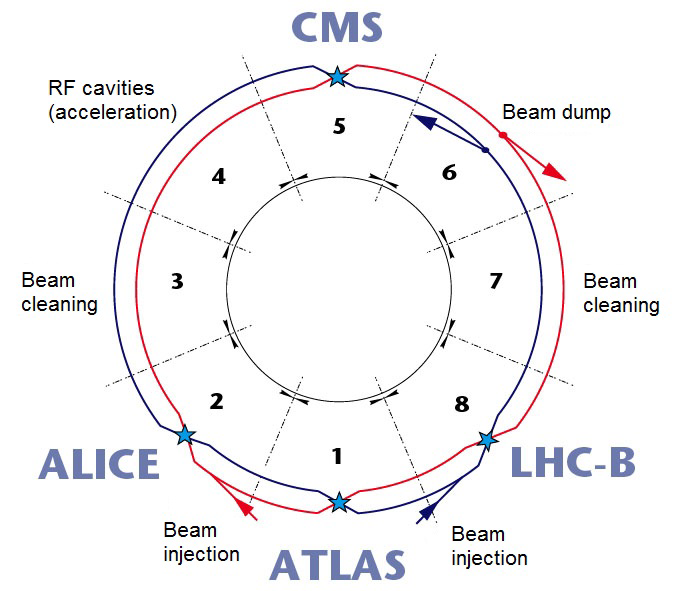
\includegraphics[width=.48\textwidth]{sections/introduction/figures/LHC_accelerator_view.png}};
    \end{tikzpicture}
    \caption{Schematic representation of the LHC~\cite{schematic_representation_lhc}.}
    \label{fig:schematic_representation_lhc}
\end{figure}

The LHC is able to accelerate protons to the energy of $E=7~\text{TeV}$ in each of two rings.  Using two separate loops serves for doubling the collision energy reaching $E=14~\text{TeV}$ at intersection points of the machine. The higher energy is attained, the deeper one can study the particle showers obtained during the impact. They allow for unravelling the fundamentals of particles and interactions between them. There are four collision points in the LHC with different dectectors installed: ATLAS\footnote{A Toroidal LHC ApparatuS}, CMS\footnote{CMS -- Compact Muon Solenoid}, ALICE\footnote{ALICE - A Large Ion Collider Experiment} and LHCb. ATLAS and CMS are two large general-purpose detectors whereas ALICE is specialised in heavy-ion physics and LHCb -- in matter-antimatter asymmetry~\cite[p.~3-21]{evans_marvel_of_technology}.

As presented in Fig.~\ref{fig:schematic_representation_lhc}, the LHC machine is divided into eight sectors. Detectors are installed in four of them. The sectors two and eight serve for inserting the preliminary accelerated beam from other CERN accelerators. In sector four, RF cavities accelerate the beam at every turn before the particles reach the desired energy. The LHC is also equipped with a beam dump system which extracts the beam from the tunnel in case of a machine failure or if the beam quality deteriorates~\cite[p.~1-4]{maciejewski_cosimulation_transient_effects_in_magnets}. 

The LHC is currently being upgraded to the High-Luminosity LHC. The project aims at increasing the frequency of particle collisions which will improve the machine performance. 

\section{Superconductors and Quench Problem}
\label{section: superconductors}

\subsection{Superconductors and Available Materials}

At the beginning of the \nth{20} century, Heike Kamerlingh Onnes liquified helium and started using it to cool down various metals to extremely low temperatures. He discovered that the resistance of solid mercury disappeared at $T=4.2~\text{K}$ and named this phenomenon a "superconductivity". Since that period, there have been many discovered materials characterised by similar physical properties. There are two main types of superconductors distinguished by the temperature at which they loose their superconducting state: 
\begin{itemize}
    \item Low-temperature superconductors (LTS).
    \item High-temperature superconductors (HTS).
\end{itemize}
LTS-based cables can operate in a superconducting state in the range of $T \in (4, 20)~\text{K}$ whereas HTS-based ones -- at higher temperatures. The HTS technology is very promising for future applications because it will enable machines for an operation at higher magnetic fields while spending less energy to cool it. However, the HTS cables still remain at the stage of research and development in most of the applications concerning accelerator magnets~\cite[p.~77-95]{evans_marvel_of_technology}. 

In order to use a superconductor in engineering applications for a magnet design, it must meet four basic requirements~\cite[p.~77-95]{evans_marvel_of_technology}:

\begin{enumerate}
    \item The material should have appropriate basic physical properties, i.e. high critical temperature and critical magnetic field.
    \item The material must be relatively common, i.e. reasonably cheap.
    \item The material must be easy to form into common shapes such as tapes or wires.
    \item The material must withstand mechanical loads inside a magnet.
\end{enumerate}

There are two low-temperature superconductors that are commercially available for~a large scale magnet production: Nb-Ti and $\text{Nb}_3 \text{Sn}$. Each of them meets most of the specified technical requirements. Nb-Ti is an alloy widely used in a magnet design due to its extreme ductility that allows for an easy cable extrusion and further winding process. $\text{Nb}_3 \text{Sn}$ is a brittle material sensitive to mechanical stresses. It requires a greater effort in coil production compared to Nb-Ti. In the fabrication process, it is initially formed to resemble its final geometry. The next manufacturing step consists of a few day high-temperature treatment during which the cable hardens and reaches its full performance. The main advantage of $\text{Nb}_3 \text{Sn}$ is its higher critical parameters of temperature and magnetic field with respect to Nb-Ti~\cite[p.~29-41]{superconducting_accelerator_magnets}.

\subsection{Critical Parameters and Stability}

As presented in Fig.~\ref{fig:scheme_critical_surface}, the superconducting state depends on three critical parameters: temperature, magnetic field and current density. These three variables create a so called "critical surface" under which a material remains in a superconducting state. The transition from the superconducting to the normal state is called a "quench". It occurs when an operating point of a superconductor remains outside of the critical surface. One can notice in Fig.~\ref{fig:scheme_critical_surface} that $\text{Nb}_3 \text{Sn}$ is characterised by a larger volume under the critical surface. Higher critical parameters of this material allow for its potential usage at stronger fields in accelerator magnets.

\begin{figure}[H]
    \centering
    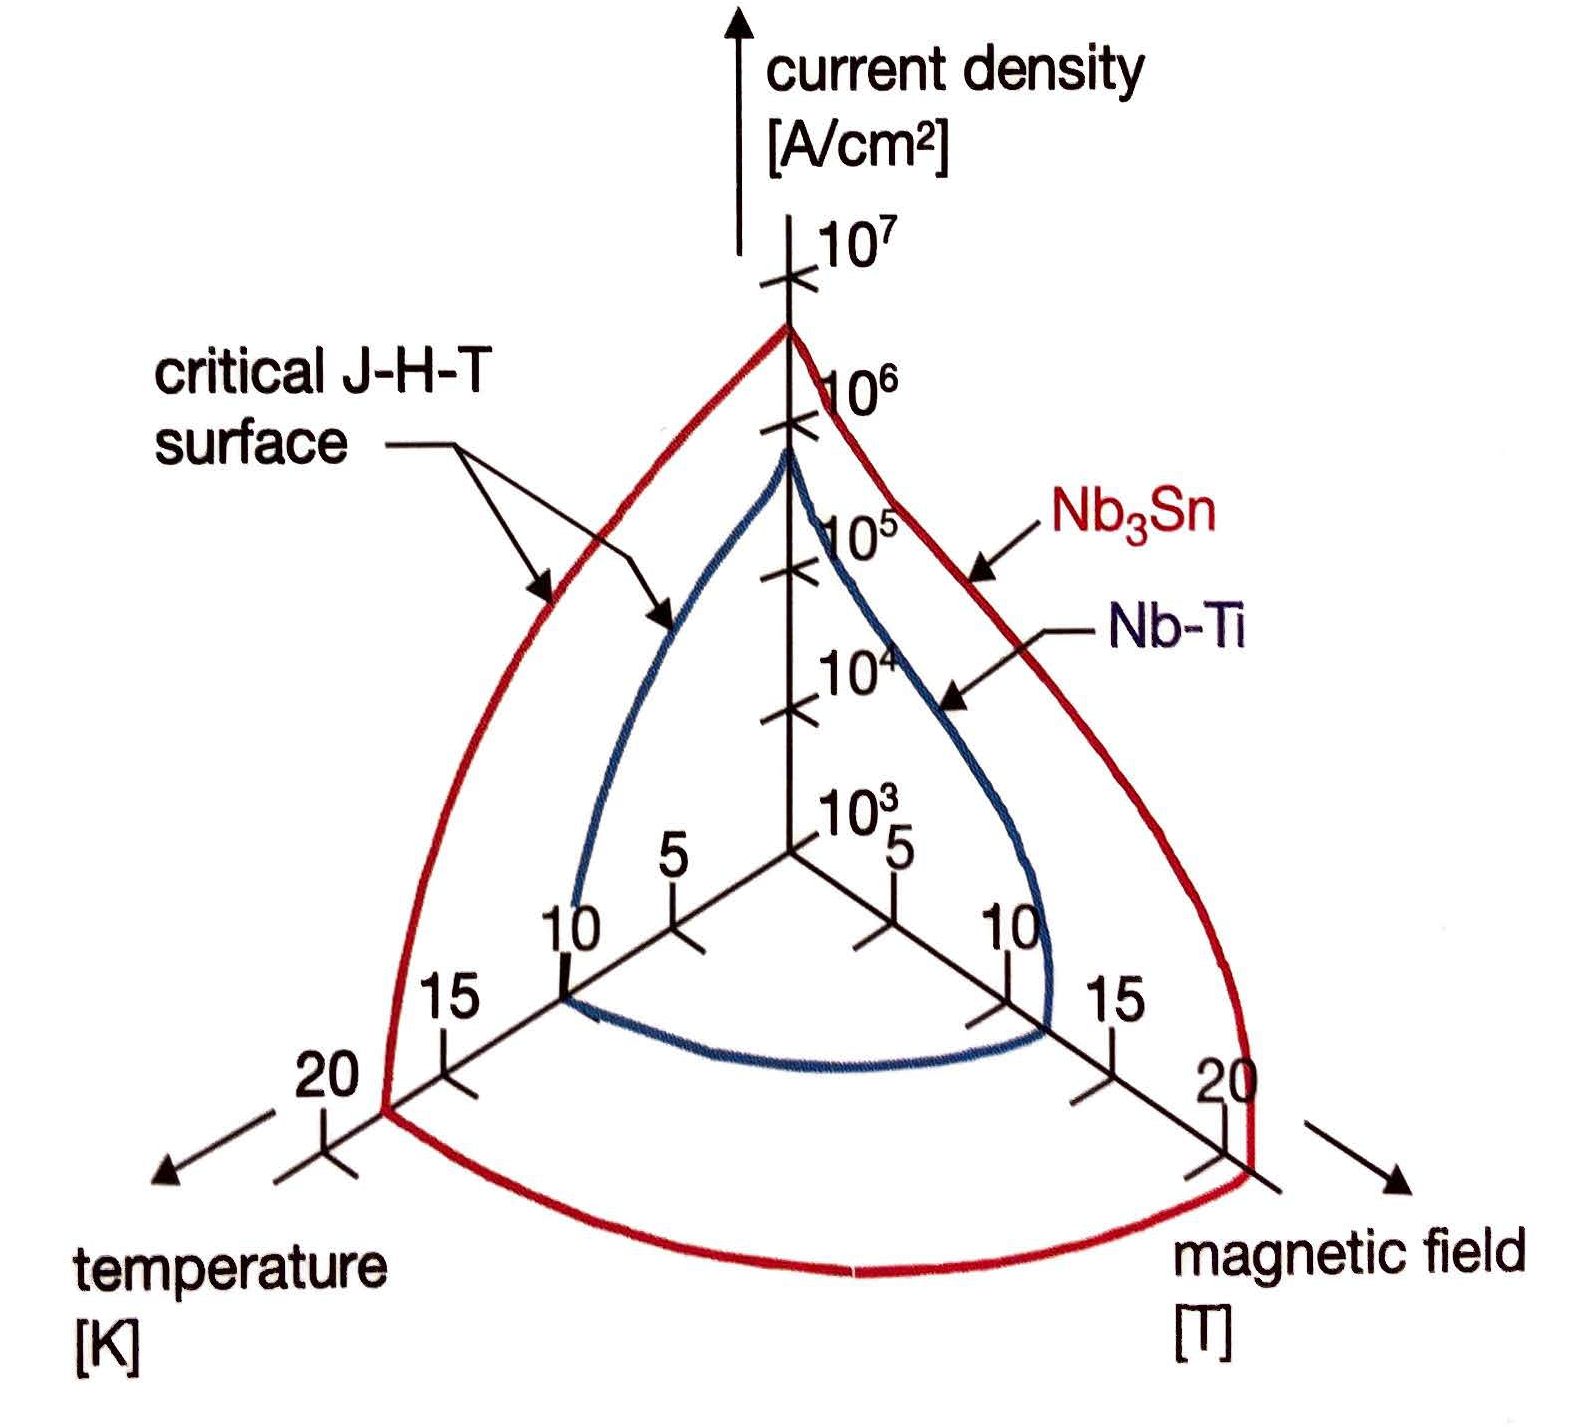
\includegraphics[width=0.35\linewidth]{sections/introduction/figures/critical_surface_scheme.png}
    \caption{Critical surface for $\text{Nb}_\text{3}\text{Sn}$ and Nb-Ti \cite{evans_marvel_of_technology}}
    \label{fig:scheme_critical_surface}
\end{figure} 

From the magnet design standpoint, it is impossible to use a superconductor alone because it is vulnerable to flux jumps. If the material exceeds its critical magnetic field, it looses its superconducting properties. A superconductor can easily reach its critical temperature as well. At temperatures close to the absolute zero, even a small energy deposition in the order of $1~\frac{\text{mJ}}{g}$ may cause a quench. It is mainly due to an extreme low heat capacity of solid materials at cryogenic temperatures (see Appendix~\ref{appendix_material_properties_description}). In addition, superconductors have relatively high resistivity in a normal conducting state with respect to the materials considered to be good electrical conductors such as copper. As described in Fig.~\ref{fig:resitivity_tin_copper}, the resistivity of tin, being a superconductor below $T_\text{c}$, is higher at normal conductive state with respect to the copper~\cite[p.~1-6]{superconducting_accelerator_magnets}.

\begin{figure}[H]
    \centering
    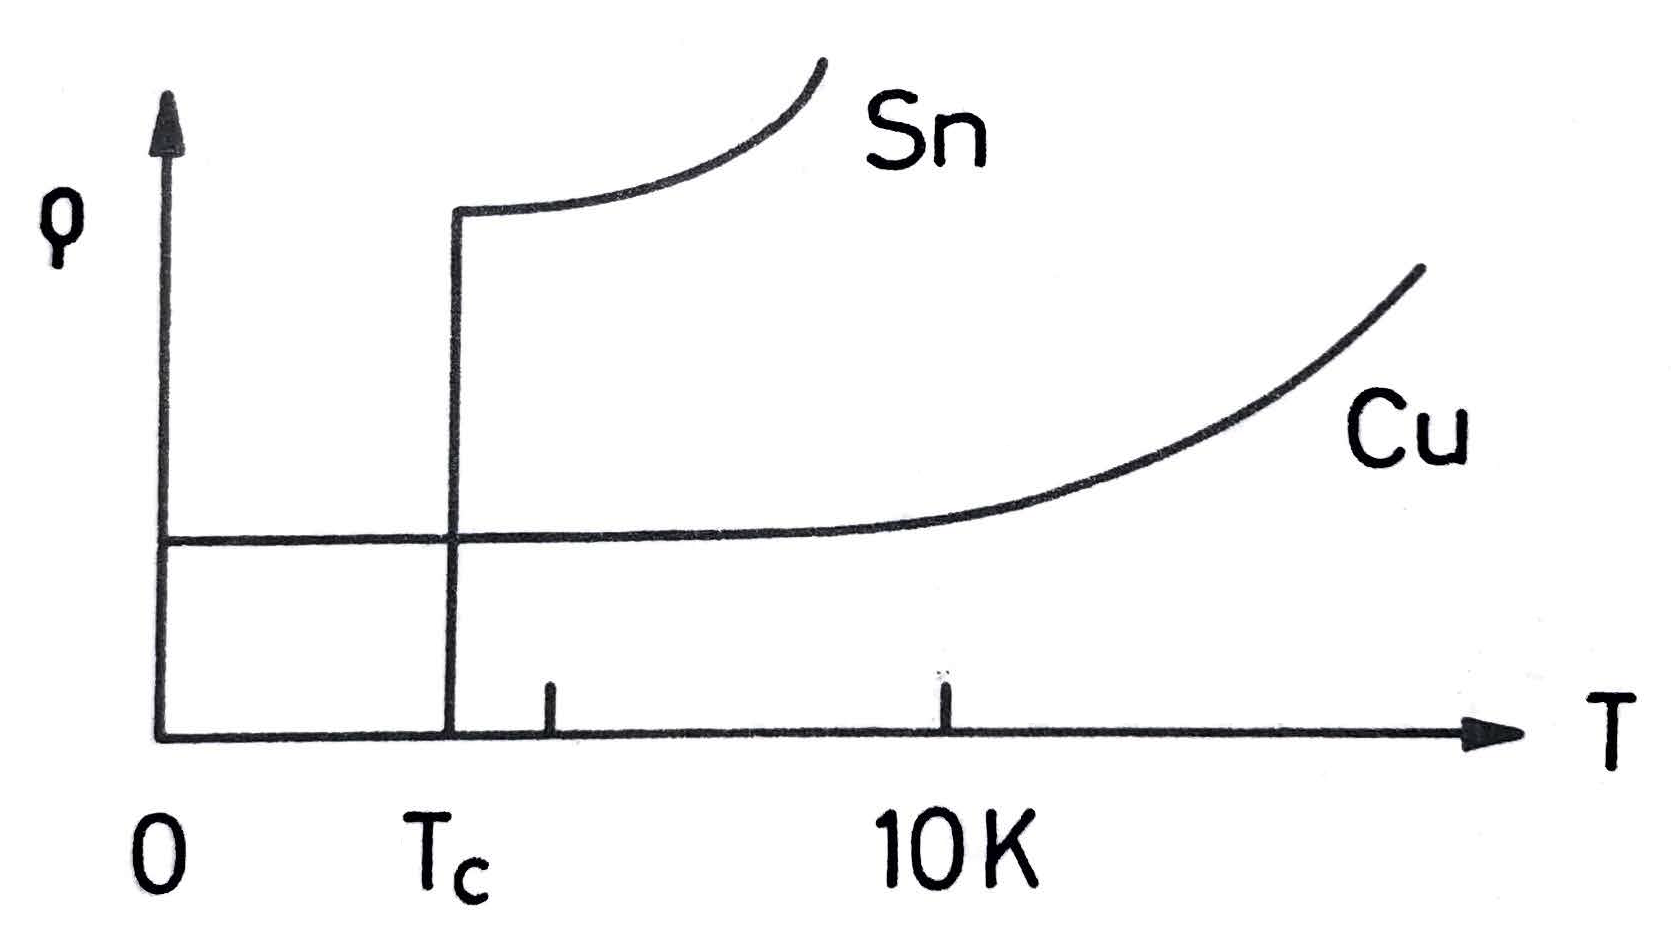
\includegraphics[width=0.35\linewidth]{sections/introduction/figures/sn_cu_resistivity.png}
    \caption{Low temperature resistivity of copper and tin~\cite{superconducting_accelerator_magnets}}
    \label{fig:resitivity_tin_copper}
\end{figure} 

In order to increase the cable stability, a superconductor is embedded in a copper matrix. When a superconductor quenches, the current bypasses it and flows through the copper characterised by a lower resistivity in a normal conducting state. During that moment, the superconductor may cool down and recover its superconducting state. The copper matrix serves for three purposes~\cite[p.~31-33]{superconducting_accelerator_magnets}: 

\begin{enumerate}
    \item Mechanical stability.
    \item Electrical bypass of high electrical conductivity.
    \item Heat sink.
\end{enumerate}

The strand composite of Nb-Ti with a copper matrix is illustrated in two pictures in Fig.~\ref{fig:strand_and_filaments}. In the left one, singular superconductor filaments are shown whereas the right one represents a cross-section of a full strand with Nb-Ti and a copper matrix. The strand diameter is usually approximately equal to 1~mm, and the diameter of a single filament -- $10~\upmu$m.
The composite fabrication should ensure a good contact between the copper and a~superconductor. The copper should also be characterised by a high residual resistivity ratio (see Appendix~\ref{appendix:subsection_rrr_definition}), i.e. it ought to be highly conductive both electrically and thermally~\cite[p.~31-33]{superconducting_accelerator_magnets}.

\begin{figure}[H]
    \centering
    \begin{tikzpicture}
    \node at (5,0) {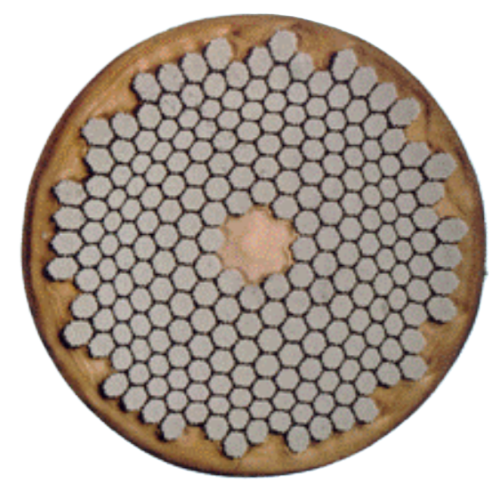
\includegraphics[width=.3\textwidth]{sections/introduction/figures/strand_cross_section.png}};
    \node at (0,0) {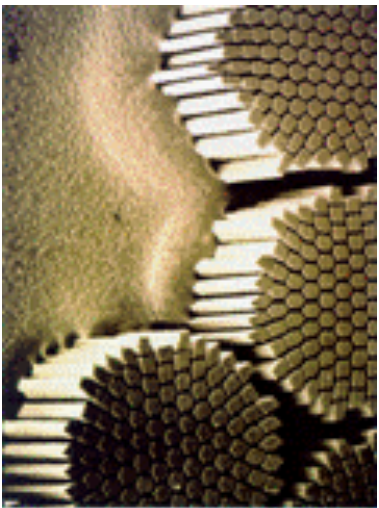
\includegraphics[width=.22\textwidth]{sections/introduction/figures/strand_filaments.png}};
    \end{tikzpicture}
    \caption{Left: Nb-Ti strand cross-section, right: filaments in the strand~\cite{lhc_machine_outreach}}
    \label{fig:strand_and_filaments}
\end{figure}

Another method to increase the strand stability is based on using a cooling liquid. Liquid helium is characterised by a high heat capacity with respect to solids at temperatures close to absolute zero. By assuring a good thermal contact between the strand and the liquid, one can strongly increase the system stability. However, in many applications the strand or a stack of strands is fully insulated with a polymer that does not enable helium to penetrate the copper matrix. In such a case, the direct contact between the liquid and the strand is negligible and cooling of a quenched zone is only possible through a longitudinal heat propagation along the strand~\cite[p.~122]{superconducting_accelerator_magnets}.

Taking into consideration a superconducting magnet as a whole composed of multiple strands, it may quench mainly because of two reasons: 
\begin{enumerate}
    \item A coil element can move in a stack of strands due to the action of Lorentz forces. The friction movement between different elements of the winding  would result in the generation of heat.
    \item According to the Faraday's Law, any change of a magnetic flux in a system creates an electromotive force, (EMF). The EMF induces eddy currents resulting in a magnetic field opposing the initial change of the magnetic flux. Since the composite strands are partially made of copper, being normal conducting at every moment of the magnet operation, excessive eddy currents can be an important heat source for a superconductor.
\end{enumerate}

\subsection{Current Sharing Phenomenon}

In reality, when an operating point of a superconductor starts approaching the critical surface, it exhibits a gradual transition to a normal conducting resistivity. This phenomenon is called current sharing. If the current in the composite strand slightly exceeds the value of a critical current, both elements of the strand become normal conducting. It is assumed that the superconductor carries the current of its critical value and the copper matrix bypasses the surplus of this value equal to $I-I_\text{c}$. In this case, the superconductor and the copper are in a parallel connection~\cite[p.~119-121]{superconducting_accelerator_magnets}. By assuming a linear dependence of $I_\text{c}$ on temperature, the critical current can be calculated as 
\begin{equation}
    I_\text{c} = I \cdot \frac{T-T_\text{cs}}{T_\text{c}-T_\text{cs}},
\end{equation}
where $I_\text{c}$ -- critical current, $I$ -- transport current in the strand, $T$ -- local temperature of the strand, $T_\text{c}$ -- critical temperature, $T_\text{cs}$ -- current sharing temperature. If the local temperature $T$ is assumed to be equal to the operating bath temperature $T_0$, one can deduce the current sharing temperature as
\begin{equation}
    T_\text{cs} = T_\text{0} + (T_\text{c} - T_\text{0}) \cdot (1 - \frac{I}{I_\text{c}~T_0}),
\end{equation}
where $T_0$ -- bath temperature of the strand. Therefore, the current in a copper matrix can be divided into three regimes as
\begin{equation}
    \left\{ \begin{array}{ lll }
    I_\text{Cu} = 0 & \text{for}~T < T_\text{cs}, \\ \\
    I_\text{Cu} = I - I_\text{c} & \text{for}~T_\text{cs} \leq T<T_\text{c},  \\ \\
    I_\text{Cu} = I & \text{for}~T_\text{cs} \leq T,
    \end{array} \right.
\end{equation}
where $I_\text{Cu}$ -- current in the copper matrix. Following the regimes for the current in the copper matrix, one can deduce three regimes for the Joule heating as
\begin{equation}
    \left\{ \begin{array}{lll}
    q_\text{Joule} = 0 & \text{for}~T < T_\text{cs}, \\ \\
    q_\text{Joule} = \frac{\rho_\text{Cu}}{f_\text{Cu}} \cdot \frac{(I-I_\text{c})^2}{{A_\text{Cu}}^2}& \text{for}~T_\text{cs} \leq T<T_\text{c},  \\ \\
    q_\text{Joule} = \frac{\rho_\text{Cu}}{f_\text{Cu}} \cdot \frac{I^2}{{A_\text{Cu}}^2} & \text{for}~T_\text{cs} \leq T,
    \end{array} \right.
\end{equation}
where $q_\text{Joule}$ -- Joule heating, $\rho_\text{Cu}$ -- local resistivity of copper, $f_\text{Cu}$ -- fraction of copper in the composite strand, $A_\text{Cu}$ -- cross-sectional area of copper in the composite strand.

\subsection{Minimum Propagating Zone}

In this section, a fully insulated strand is analysed, i.e. the influence of helium in quench propagation is negligible. In the given consideration, the following assumptions are made: 
\begin{itemize}
    \item The strand is only made of a superconductor without a copper stabiliser. 
    \item The current density in the wire is close to its critical value. 
    \item The length $L$ of a superconductor is heated from the bath temperature $T_0$ to the temperature $T$ above the critical value $T_\text{c}$.
\end{itemize}

Since helium is not considered, the thermal disturbance in the strand leads to the quench propagation if the longitudinal heat evacuation is lower than the generation of heat in the quenched zone. It is formulated as
\begin{equation}
    \rho J^2 A L \geq \frac{kA(T_\text{c}-T_0)}{L},
\end{equation}
where $J$ -- current density, $A$ -- wire cross-section, $L$ -- heated length of a superconductor, $k$~-- thermal conductivity of the wire, $T_\text{c}$ -- critical temperature, $T_0$ -- bath temperature. One can simply deduce the minimum propagating zone from the equation as
\begin{equation}
    L_\text{MPZ} = \sqrt{\frac{2k(T_\text{c}-T_0)}{\rho J^2}}.
\end{equation}
If the thermal disturbance is larger or equal to $L_\text{MPZ}$, the quench starts propagating along the wire. For pure Nb-Ti, the $L_\text{MPZ}$ is approximately equal to $L=1~\upmu \text{m}$. Such a~small value explains why a~copper stabiliser is necessary in a composite strand. The usage of copper may increase $L_\text{MPZ}$ by a factor of thousand~\cite[p.~124]{superconducting_accelerator_magnets}. 

\section{Accelerator Magnets}
\label{section: accelerator_magnets}

\subsection{Types and Functions}

In the LHC, there are various accelerator magnets which can be divided into three main groups based on their function~\cite{cern_main_webpage}: 
\begin{enumerate}
    \item Main dipole magnets. They bend the moving particles in order to keep them in the trajectory of a 27 km-long ring of the LHC. There are 1232 dipoles in the LHC.
    \item Main quadrupole magnets. They constrain the width and the height of a particle beam in order to maintain it inside of the vacuum chamber within the LHC magnet. There are 392 such magnets inside the LHC.
    \item Corrector magnets. One of their goals is to correct imperfections in the field quality created in the aforementioned magnets. Some of the examples of such magnets are: quadrupoles and skew quadrupoles, sextu-, octu-, deca- or dodecapoles. 
\end{enumerate}

Figure~\ref{fig:cross_section_lhc_main_dipole} presents the cross-section of the main LHC dipole. The particle beam is travelling inside of a beam pipe surrounded by a double-layer coil composed of multiple turns of a~superconducting cable. The coils are clamped with pre-stressed steel collars in order to oppose the Lorentz forces acting on them during the machine operation. Since the magnets are mounted at room temperature, the pre-stress also serves for maintaining the elements position when the entire structure shrinks during the cooling process. In principle, the pre-stress maintains the contact between the coil and neighbouring elements which allows for avoiding friction and, thus, the heat generation. The collars are surrounded by a concentrically mounted iron yoke. The iron yoke increases the central magnetic field that directs the~travelling beam.

\begin{figure}[H]
    \centering
    \begin{tikzpicture}
    \node at (0,0) {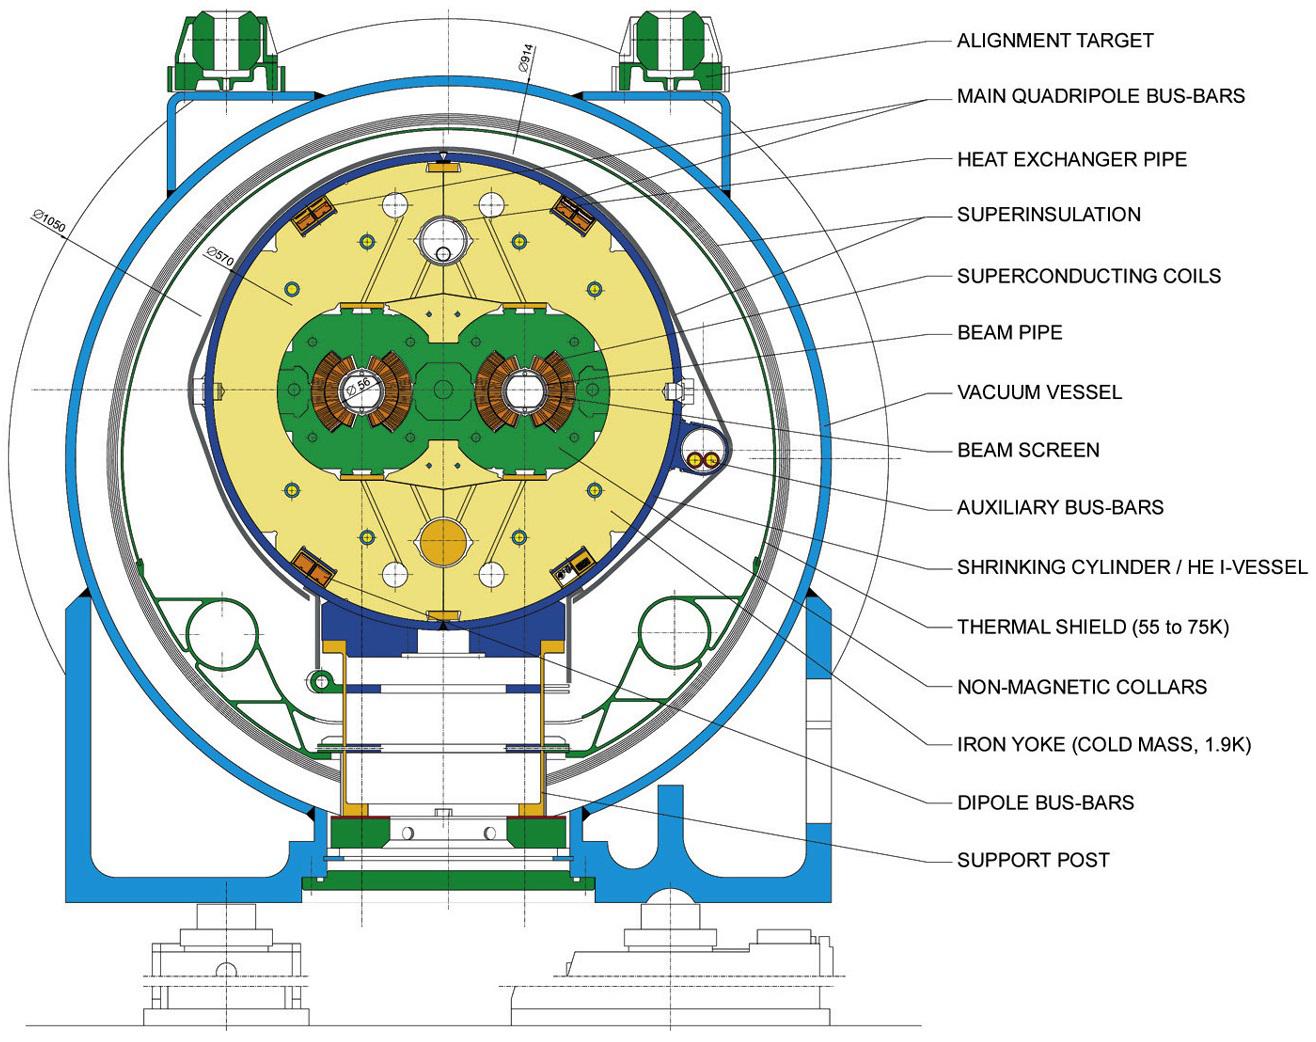
\includegraphics[width=.75\textwidth]{sections/introduction/figures/LHC_main_dipole_cross_section.png}};
    \end{tikzpicture}
    \caption{Cross-section of the LHC main dipole magnet with description of main components~\cite{lhc_main_dipole_cross_section}.}
    \label{fig:cross_section_lhc_main_dipole}
\end{figure}

\subsection{Quench Protection}

When a quench occurs during the operation of a superconducting magnet, it~must be detected in the shortest possible time. As soon as the quench is detected, the~power converter, that supplies with current magnets connected in series, is switched off and energy, mostly magnetic, stored in the circuit is discharged. In principle, the energy should be either deposited in the coil or extracted from the magnet. The quench protection systems can be passive or active. The passive systems do not use any additional electronics which triggers the quench protection devices. An example of a passive protection system is a diode connected in parallel to a~magnet. When the quench occurs, both the diode and the magnet are subjected to the same resistive voltage. If the resistive voltage reaches the forward diode voltage, the diode allows the current to bypass the magnet.

Among others, three active protection systems are described: 

\begin{enumerate}
    \item Quench heaters
	\item Coupling-Loss Induced Quench (CLIQ) system
	\item Energy extraction
\end{enumerate}

Quench heaters are resistive strips installed along the coils in close contact with the~windings. The heaters have an external power supply usually based on a charged capacitor. When a quench is detected, the heaters are fired. Due to the firing of the protection system, the quench heater spots, being in close contact with the windings, quench inside of a coil. This process supports the longitudinal quench propagation initiated at each of the quench heater spots. A~larger resistive volume is created in the magnet and the current discharge occurs more quickly. The quench heaters have an external power supply independent of the superconducting coils. Therefore, they must be electrically insulated from the windings. In fact, the electrical insulation is a thermal barrier causing a~delay between the moment when the heaters are fired and the time when the coil quenches. This delay is a characteristic feature of a quench heater system. The~drawbacks of the quench heaters are as follows~\cite{salmiquenchheateroptimization}: 

\begin{enumerate}
    \item On one hand, the quench heater system requires a high thermal diffusivity, i.e. the~insulation between the heater and the coil should be thin enough to decrease the delay of the firing system. Meanwhile, the system should meet the requirements of an electrical insulator, which should be thick enough to prevent short-circuits. These two requirements are contradictory with respect to one another. 
	\item There is no possibility to replace quench heating strips of the magnet once they are installed. Therefore, in case a failure during the machine operation, the maintenance of this system is limited in a~long-term. 
\end{enumerate}

In addition, there exists a natural effect that enables a magnet to discharge quicker, called a “quench back”. According to the Faraday’s law, the variation of a magnetic field in time induces eddy currents in an electrical conductor. The heat generated due to this phenomenon is referred as AC-losses. If the current drops sufficiently quickly, the AC-losses may induce a quench in the parts of a coil which remain superconducting. The CLIQ system is based on the same physical principle. It generates current oscillations in the superconducting windings to create a fast change of the magnetic field. According to~\cite{ravaioli_cliq_phd_thesis}, the CLIQ protection is more efficient with respect to the quench heaters in the operating conditions of a magnet close to the critical surface. CLIQ is implemented as a baseline for the inner triplets\footnote{Inner triplets provide the final focusing of the proton beams at four collision points of the LHC~\cite{lhc_inner_triplet_powering_strategy}.} for the HL-LHC project.

In the energy extraction system, a dump resistor is connected in series to a set of superconducting magnets in a circuit. When the~quench is detected, an active switch allowing the current to bypass the dump resistor is disconnected.  Thus, a~part of the energy stored in the circuit is discharged in the resistor. This system allows for a faster recovery of a magnet to its operating conditions because it requires less cooling power after the discharge process.~\cite{salmiquenchheateroptimization}

A superconducting magnet can also be "self-protected" meaning that the energy accumulated in the circuit is discharged by a natural rise of resistivity inside of the magnet. This is the simplest and most cost-effective solution. The self-protectability is applicable in magnets characterised by relatively low current densities and, therefore, low magnetic fields. A~relatively small amount of discharged energy in these magnets allows for limiting the temperature rise during the quench. In principle, the self-protectability should be the baseline for the magnet protection. However, if the energy density is too high, one should opt for an additional protection equipment.

\subsection{Magnet Design Key Parameters}

From the magnet design standpoint, the key parameters are:
\begin{enumerate}
    \item peak voltage to ground
    \item maximum hot-spot temperature
\end{enumerate}

Temperature is rarely measured in experiments because there is no space to mount temperature sensors within the magnets. It is physically deduced from the resistive voltage measured across the magnet as a quench propagates. The place where a quench starts propagating is characterised by the highest temperature in the entire magnet during quench (also referred as the hot-spot temperature). The rise of resistive voltage inside the magnet must also remain within the allowable voltage-to-ground limits as well as turn-to-turn voltage limits imposed by electrical properties of the insulation. Exceeding these limits may lead to:

\begin{enumerate}
    \item Short-circuit between different windings of the coil across the internal windings' insulation,
    \item Short-circuit between the winding and the ground across the ground insulation of the magnet.
\end{enumerate}

The hot-spot temperature and the voltage-to-ground value allow for defining whether the materials reach their safety limits at which they loose mechanical, thermal or electro-magnetic properties leading to the magnet destruction. Therefore, there is a need to study the evolution of the key parameters in the process of a magnet design when the quench occurs in the considered system.

\section{Numerical Analyses in Superconductors}
\label{section: numerical_analyses_in_superconductors}

\subsubsection{Thermal Numerical Analyses}

To write in introduction: 
Wilson: \\
- point disturbances (page 74) \\
- minimum propagating zone (MPZ) (same page - up to 80 something...)

% AIM THESIS
\clearpage \thispagestyle{empty}
\chapter{Aim of Thesis}
\label{chapter: aim_thesis}

\section{Research Objectives}

Solving temperature distribution in a superconducting magnet in 3D where quench is considered is a challenging task. The~reasons standing behind this are twofold: $(i)$~nonlinear material properties at cryogenic temperatures; $(ii)$~high temperature gradients at the quench front. When a numerical solver deals with the problem characterised as follows, it decreases its time step in order to reach convergence. It also requires a finer mesh to represent the steep temperature change at the quench front. Both implications make the simulation computationally demanding. A good example of the level of non-linearities at cryogenic temperatures is thermal conductivity of copper. Its value changes from 250 to 1700 $\frac{\text{W}}{\text{m K}}$ at $T \in (1.9, 20)~\text{K}$ for $B=3~\text{T}$ according to NIST\footnote{NIST -- National Institute of Standards and Technology} \cite[p.~9-13]{material_properties_roxie}.

Since the 3D thermal models are computationally demanding, they are not suitable for use in magnet design which is an intrinsically iterative process. In this thesis, there are two scientific questions asked:

\begin{enumerate}
\item Can a multidimensional thermal analysis in superconducting accelerator magnets be more efficient computationally?
\item  Can such an optimised modelling for superconducting accelerator magnets be conducted in ANSYS which is nowadays one of the most widespread commercial tools for FEM numerical simulations on the market?
\end{enumerate}

One can ask a question whether there exist methods for approximating the quench problem which would allow for obtaining quick and reliable solution. If the quench position in time was known a priori and estimated beforehand, the numerical solver would solve the temperature distribution faster over the coil domain. Such an approach has been inspired by ITER's Magnet Division approach to quench modelling of toroidal superconducting magnets in fusion applications~\cite{iter_presentation_qualified_analysis, iter_fault_case_study}. In this thesis, this method, called quench velocity modelling, is applied for the case of accelerator superconducting magnets. 


\section{Thesis Structure}

The thesis is divided as follows. Chapter~\ref{chapter: introduction} is a general introduction to the quench analysis in superconducting magnets that allows the reader to smoothly acquaint with the problematics of the thesis. Chapter~\ref{chapter: aim_thesis} depicts the main objectives of this work. Since at TE-MPE-PE section\footnote{TE-MPE-PE is an abbreviation for Performance Evaluation Section belonging to Machine Protection and Electrical Integrity Group being part of Technology Department at CERN.}, COMSOL is used as the standard software for solving thermal quench problems, in Chapter~\ref{chapter: 1d_quench_propagation_modelling}, 1D quench propagation is solved in both ANSYS and COMSOL to cross-check the results. The analyses of a 1D strand are conducted with and without an insulation layer and resin. Chapter~\ref{chapter:quench_velocity_modelling} explains in detail the quench velocity-based approach to solve multi-dimensional thermal problems in superconducting magnets.
Chapter~\ref{chapter:algorithms} describes the algorithms created to perform a multi-dimensional thermal analysis. Chapter~\ref{chapter:python_implementation} deals with how the foregoing algorithms are implemented in the simulations through Python scripts and as well as in ANSYS APDL scripts. Chapter~\ref{chapter:quench_velocity_benchmarking} compares the quench velocity-based approach with standard analyses performed in Chapter~\ref{chapter: 1d_quench_propagation_modelling}. In Chapter~\ref{chapter:skew_quadrupole_quench_detection_analysis}, the quench velocity-based approach is applied to solve a multi-dimensional thermal problem of a skew quadrupole, being one of the high-order corrector magnets for the High-Luminosity LHC upgrade. The analysis is performed: $(i)$ at constant current to simulate the quench propagation until the quench is detected, $(ii)$ at varying current during the magnet discharge after the quench detection. The simulation results are compared with available measurements. Chapter~\ref{chapter:research_questions_discussions} summarises the covered topics as well provides an answer to the research questions proposed in this thesis.



% 1D QUENCH PROPAGATION MODELLING 
\clearpage
\chapter{1D Quench Propagation Modelling}
\label{chapter: 1d_quench_propagation_modelling}

\section{Motivation}
\label{section: 1d_quench_propagation_motivation}

At TE-MPE-PE section, the standard software to solve 1D heat propagation problems related to quench is COMSOL. In the \nth{1} step of the quench studies, simplified ANSYS models are verified by means of STEAM-BBQ being a tool implemented in COMSOL and developed in the section \cite{BBQ_manual}. The main aim of this cross-check is to verify the validity of implemented physics in ANSYS with respect to COMSOL. The presented studies are based on previously implemented 1D models in ANSYS where the influence of helium on the quench propagation is analysed~\cite{paudel_thesis}. A chapter of that work includes the comparison of COMSOL and ANSYS when an adiabatic 1D quench propagation is considered without an insulation layer~\cite{paudel_thesis} .


\section{Assumptions}
\label{section: 1d_quench_propagation_assumptions}

In this chapter, there are two studies conducted for a quench propagation in a 1D strand: 

\begin{enumerate}
    \item Analysis of a bare composite strand
    \item Analysis of the composite strand with insulation and epoxy resin
\end{enumerate}

For both cases, the mesh density study is conducted. The following assumptions are made in the simulations: 

\begin{enumerate}
    \item There is no helium cooling.
    \item Temperature in the cross-section of a composite strand is uniform.
    \item Turn-to-turn propagation does not occur between different windings of a coil.
    \item When the insulation and epoxy resin are considered, the longitudinal heat transfer outside of the bare strand is neglected.
\end{enumerate}

The second and third assumptions allow one to consider the quench simulation as a 1D longitudinal heat propagation. When the strand is analysed with an external insulation and epoxy resin, the analysis becomes a 1D+1D heat conduction problem because of the fourth assumption. It is further explained in Section \ref{section: 1D_quench_propagation_with_insulation}. In presented thermal problems, the heat balance partial differential equation is solved as
\begin{equation}
    \gamma c_p(T,B) \frac{\partial T}{\partial t} = \frac{\partial}{\partial \vec{r}}[k(T,B) \frac{\partial T}{\partial \vec{r}}] + q_0(T,B),
    \label{eqn:PDE_heat_balance}
\end{equation}
where $T$ -- temperature varying in time and space defined by a position vector $\vec{r}$, $\gamma$ -- mass density of a material, $c_p$ -- specific heat of a material, $k$ -- thermal conductivity of a material, $q_v$~-- external heat source (Joule heating). Specific heat capacity, thermal conductivity, and resistivity are a function of both temperature and magnetic field strength in the strand. The insulation of the strand and, optionally, resin are only a function of temperature. The domain is thermally anisotropic when the superconducting strand is analysed with an external insulation layer and, optionally, epoxy resin.

\section{Reference Geometry - Skew Quadrupole}
\label{section: 1d_quench_propagation_geometry}

In this thesis, all the simulations are based on the geometry of a skew quadrupole which belongs to the group of high-order corrector magnets designed for the High-Luminosity LHC upgrade. The skew quadrupole is developed by the LASA laboratory of INFN-Milano. Its geometry is presented in Fig. \ref{fig:Skew_quad_geometry}. Each coil of the skew quadrupole (marked in red in the left picture) is fully impregnated and positioned in two mechanical supports (marked in grey). The entire magnet is surrounded by an iron yoke (marked in blue). One coil of a magnet out of four in total is presented in the right picture.

\begin{figure}[H]
    \centering
    \begin{tikzpicture}
    \node at (0,0) {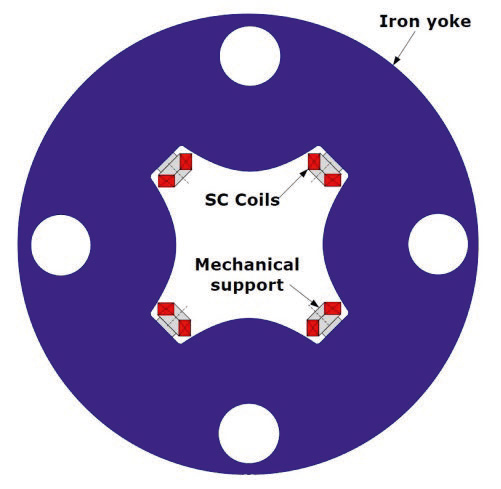
\includegraphics[width=0.3\linewidth]{sections/1D_quench_modelling/figures/geometry/Quadrupole_Cross_Section.png}};
    \node at (5,0) {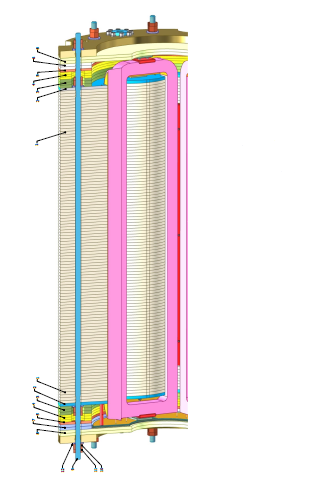
\includegraphics[width=0.225\linewidth]{sections/1D_quench_modelling/figures/geometry/SkewQuad3D.png}};
    \end{tikzpicture}
     \caption{Left: cross-section of the skew quadrupole~\cite[p.~103-105]{hl_lhc_tech_design_report_v01}; right: one coil of the skew quadrupole~\cite{marco_prioli_mails}.}
    \label{fig:Skew_quad_geometry}
\end{figure}

As presented in Fig.~\ref{fig: 1d_strand_geometry}, the coil consists of a composite strand marked in yellow made of Nb-Ti and a copper stabiliser. The strand is fully insulated with an S2-glass material marked in red. The cable is wound 754 times to form a coil with the total length of 812~m~\cite{samuele_mariotto_mails}. After the winding process, the coil is impregnated with an epoxy resin CTD-101K marked in blue in Fig.~\ref{fig: 1d_strand_geometry}. The Rutherford cable is not applied in high-order corrector magnets. In the remainder of the thesis, the term "cable" is restricted to the composite strand made of a superconductor and a copper stabiliser including an external insulation layer and, optionally, a resin filler. The bare cable and winding are referred to as "strand". The one-dimensional coordinate system $\bar x$ in Fig.~\ref{fig: 1d_strand_geometry} represents the longitudinal direction of the strand. The 1D geometry is based on geometrical parameters of a single strand of the skew quadrupole whose simulations are further described in the next section. 

\begin{figure}[H]
    \centering
    \begin{tikzpicture}[scale = 1]
        \filldraw[blue] (-0.941,-0.941) rectangle (0.941,0.941);
        \filldraw[red] (0,0) circle (0.7+0.07*2);
        \filldraw[yellow] (0,0) circle (0.7);
        \draw[thick, cyan] (-0.8*1.5,0.7) -- (0,0.7);
        \draw[thick, cyan] (-0.8*1.5,-0.7) -- (0,-0.7);
        \draw[black, thick, <->] (-0.75*1.6,0.7) -- (-0.75*1.6,-0.7);
        \node[scale = 1, rotate=90] at (-1.1*1.45, 0) {$d_\text{strand}$};
        \draw[thick,<->] (-0.941,-0.9*1.5) -- (0.941,-0.9*1.5);
        \node[scale = 1] at (0, -0.7*1.6) {$a$};
        \draw[thick,->] (1.5,0) -- (10.0,0);
        \draw[thin] (1.75,-0.15) -- (1.75,0.15);
        \draw[thin] (9,-0.15) -- (9,0.15);
        
        \node[scale = 1] at (9.75, 0.3) {$\bar x$};
        \node[scale = 1] at (9, -0.4) {$L_\text{strand}$};
        \node[scale = 1] at (1.75, -0.4) {0};
        
    \end{tikzpicture}
    \caption{1D strand geometry.}
    \label{fig: 1d_strand_geometry}
\end{figure}

The parameters of the skew quadrupole presented in Table \ref{table:skew_quad_params_table_basic} do not change in the remainder of the thesis. The last two: $(i)$ residual resistivity ratio, RRR, $(ii)$ copper-to-superconductor ratio, $r_\text{Cu/sc}$ are obtained from the measurements of the prototype magnet performed at INFN.~\cite{marco_prioli_mails}

\begin{table}[H]
    \caption{Geometrical parameters of the skew quadrupole \cite{hl_lhc_tech_design_report_v01, marco_prioli_mails}.} 
    \vspace{-1.em} 
    \fontsize{10}{10}
    \selectfont 
    \renewcommand{\arraystretch}{1.5}
    \begin{center}
    \begin{tabular}{ ccc }  
    \hline
    parameter & value & unit \\
    \hline
    $d_\text{strand}$ & 0.7 & [mm] \\
    $a$ & 0.941 & [mm] \\
    $r_\text{Cu/sc}$ & 2.2 & [-] \\
    RRR & 193 & [-] \\  
    \hline 
    \end{tabular}
    \end{center}  
     \label{table:skew_quad_params_table_basic} 
 \end{table}


\section{1D Analysis of a Strand}

This analysis presents the case for a bare strand, i.e. when neither insulation nor epoxy resin are considered. Therefore, the strand cross-sectional area is a yellow part of the domain presented in Fig. \ref{fig: 1d_strand_geometry}. The length of the considered domain is $L_\text{strand}=1~\text{m}$.
\label{section: 1D_quench_propagation_no_insulation}

\subsection{Geometry, Material Properties and Mesh}

Since copper and Nb-Ti are characterised by a~different volumetric heat capacity, the total volumetric heat capacity of a strand is given by

\begin{equation}
    c_\text{v, strand} = f_\text{Cu} ~ c_\text{v, Cu}(T) + f_\text{Nb-Ti} ~ c_\text{v, Nb-Ti}(T,B),
    \label{eqn: cv_equiv}
\end{equation}
where $c_\text{v, Cu}$ -- volumetric heat capacity of copper as a function of temperature, $c_\text{v, Nb-Ti}$ -- volumetric heat capacity of Nb-Ti as a function of temperature and magnetic field, $f_\text{Cu}$ -- volumetric fraction of copper, $f_\text{Nb-Ti}$ -- volumetric fraction of Nb-Ti. The~volumetric heat capacity of the composite strand for a given value of $B$ and $r_\text{Cu/sc}$ is shown in Fig. \ref{fig:eq_wind_cp}.

\begin{figure}[H]
\centering
    \begin{tikzpicture}
        \begin{axis}[
          no markers,
          width=0.7\linewidth, 
          height = 4.5cm,
          xlabel={$T,~\text{K}$},
          ylabel={$c_\text{v, strand},~\frac{\text{J}}{\text{m}^3 \cdot \text{K}}$},
          xmin=0.0,
          ymin=0.0,
          xmax=300.0
          ]
          \addplot table[x=temperature,y=cv_equiv,col sep=comma] {sections/1D_quench_modelling/figures/other/cv_equivalent.csv}; 
        \end{axis}
    \end{tikzpicture}
    \caption{Strand volumetric heat capacity as a function of temperature for $B=2~\text{T}$ and $r_\text{Cu/sc}=2.2$.}
    \label{fig:eq_wind_cp}
\end{figure}

According to~\cite[p.~46]{material_props_for_heat_transfer_modelling_in_nb3sn_magnets}, the thermal conductivity of Nb-Ti changes from 1 to 9~$\frac{\text{W}}{\text{m K}}$ in the temperature range of $T \in (20, 200)~\text{K}$. At temperatures below 20~K, the thermal conductivity of Nb-Ti is lower than~$1~\frac{\text{W}}{\text{m K}}$. By comparing the thermal conductivity of Nb-Ti and copper, whose thermal conductivity is presented in Appendix~\ref{subsection:copper_thermal_conductivity}, one can conclude that the thermal conductivity of Nb-Ti is negligible and only the part of copper contributes to the longitudinal heat propagation, as 
\begin{equation}
    k_\text{strand} = f_\text{Cu} ~ k_\text{Cu} + f_\text{Nb-Ti} ~ k_\text{Nb-Ti} \approx  f_\text{Cu} ~ k_\text{Cu},
    \label{eqn: k_equiv}
\end{equation}
where $k_\text{strand}$ -- thermal conductivity of a strand, $k_\text{Cu}$ -- thermal conductivity of copper, $k_\text{Nb-Ti}$ -- thermal conductivity of Nb-Ti. It is important to highlight that only in Chapter~\ref{chapter: 1d_quench_propagation_modelling}, the thermal conductivity of copper is calculated according to the Wiedemann-Franz formula, as
\begin{equation}
    k_\text{Cu} = 2.45 \cdot 10^{-8} ~ \frac{T}{\rho_\text{Cu}}.
    \label{eqn: k_cu_wiedemann_franz}
\end{equation}
Wiedeman-Franz formula is used for the sake of comparison of the results with COMSOL in which only such material property is available. In the remainder of the thesis, the thermal conductivity of copper and all other material properties are calculated according to the fits provided by NIST, as described in Appendix~\ref{appendix_material_properties_description}. 

In ANSYS, the element LINK33 is used to the 1D quench propagation. It is a uniaxial 2-node linear element with the ability to conduct heat between its nodes suitable for steady-state and transient analyses~\cite{ansys_element_manual}. Unlike ANSYS, COMSOL does not use explicit element types to define physical equations in a domain. Instead, one has to choose from a list of available physics modules, in this case thermal physics. Therefore, the algebraic physical equations related to heat conduction in COMSOL are applied to the nodes belonging to the composite strand. In both tools, a uniformly distributed mesh is used with mesh size equal to 0.1 mm. The mesh size is based on~\cite[p.~40]{paudel_thesis} in which it is recommended to discretise the domain in the scale less than or equal to 1~mm for an adiabatic analysis of a 1D quench propagation.

\subsection{Initial and Boundary Conditions, and Solver Settings}

Over the entire length of the strand, the power density is applied according to~(\ref{eqn: p_dens_equiv}). In addition, a Gaussian profile of the initial temperature is assumed according to 
\begin{equation}
    T(x) = T_\text{init} + (T_\text{max} - T_\text{init}) ~ e^{-(\frac{x}{\alpha})^2},
    \label{eqn: gaussian_temp_ic}
\end{equation}
where $T(x)$ -- temperature profile along $x$-axis, $T_\text{init}$ -- initial bath temperature of a strand, $T_\text{max}$ -- the maximum temperature of the Gaussian profile, $\alpha$ -- shape parameter of the Gaussian profile proportional to the standard deviation. The input parameters corresponding to the Gaussian profile, initial transport current, and initially quenched zone are depicted in Table~\ref{table: 1d_quench_propagation_analysis_init_temp_input_parameters}. 

\begin{table}[H]
    \caption{Input parameters for the 1D analysis.} 
    \vspace{-1.em} 
    \fontsize{10}{10}
    \selectfont 
    \renewcommand{\arraystretch}{1.5}
    \begin{center}
        \begin{tabular}{ ccc }  
        \hline
        parameter & value & unit \\
        \hline
        $I$ & 100 & [A] \\
        $B$ & 2 & [T] \\
        $T_\text{init}$ & 1.9 & [K] \\
        $T_\text{max}$ & 20.0 & [K] \\
        $T_\text{c}$ & 8.429 & [K] \\
        $L_\text{quench, init}$ & 0.1 & [m] \\ 
        $\alpha$ & 0.223 & [m] \\   
        \hline 
        \end{tabular}
    \end{center}  
     \label{table: 1d_quench_propagation_analysis_init_temp_input_parameters} 
 \end{table}

The initially quenched zone is equal to $L_\text{quench, init}= 0.1~\text{m}$ when symmetry is not taken into consideration. It~means that at $x=0.05~\text{m}$, the strand is at the critical temperature for the given magnetic field strength. The shape parameter, \textalpha~in (\ref{eqn: gaussian_temp_ic}) is calculated accordingly. The critical temperature $T_\text{c}$ is calculated as in (\ref{eqn:critical_temperature_appendix}) in Appendix~\ref{appendix:nbti_material_properties}. A symmetry condition is applied at the position $x=0~\text{m}$. Thus, a one metre-long strand represents a half of the analysed domain, as presented in Fig. \ref{fig: init_gauss_temp_distr}.

\begin{figure}[H]
\centering
    \begin{tikzpicture}
        \begin{axis}[
          no markers,
          width=0.7\linewidth, 
          height = 4.5cm,
          xlabel={$L_\text{strand},~\text{m}$},
          ylabel={$T,~\text{K}$},
          xmin=0.0,
          ymin=0.0,
          xmax=1.0
          ]
          \addplot table[x=posx,y=temperature,col sep=comma] {sections/1D_quench_modelling/figures/other/gaus_init_distr.csv}; 
        \end{axis}
    \end{tikzpicture}
    \caption{Initial Gaussian temperature distribution.}
    \label{fig: init_gauss_temp_distr}
\end{figure}

The solution in both ANSYS and COMSOL are obtained with a strict time stepping, i.e. the time step during the solution is fixed. The input parameters related to the time stepping algorithm and the total simulation time are presented in Table \ref{table: 1d_quench_propagation_analysis_time_stepping_input_parameters}. ANSYS uses a default sparse solver with an automatic solution control setting. In COMSOL, the Multifrontal Massively Parallel Sparse Direct Solver (MUMPS) is applied. Both tools use direct solvers with an implicit Backward Euler time stepping method~\cite{comsol_webpage, ansys_command_reference}. In a time-dependent domain, default values for time stepping convergence are applied in both ANSYS and COMSOL. The geometry is built based on the \nth{1} order elements in each tool.

\begin{table}[H]
    \caption{Analysis time stepping input parameters.} 
    \vspace{-1.em} 
    \fontsize{10}{10}
    \selectfont 
    \renewcommand{\arraystretch}{1.5}
    \begin{center}
        \begin{tabular}{ ccc }  
        \hline
        parameter & value & unit \\
        \hline
        $t_\text{total}$ & $10^{-1}$ & [s] \\   
        $t_\text{step, max}$ & $10^{-4}$ & [s] \\   
        \hline 
        \end{tabular}
    \end{center}  
     \label{table: 1d_quench_propagation_analysis_time_stepping_input_parameters} 
 \end{table}

\subsection{Results}
\label{subsubsection:1d_quench_propagation_analysis_results_no_insulation}

The temperature distribution profiles are compared at three time steps $t=\{0.03, 0.06, 0.1\}$~s, as presented in Fig.~\ref{fig: 1d_no_insulation_temp_along_strand_comparison}. One can conclude that the initial heat pulse is sufficient to initiate quench. In fact, relatively high thermal conductivity and low heat capacity of the strand allow for a longitudinal quench propagation. At each time window, the hot-spot is placed at $x=0~\text{m}$. In general, COMSOL predicts faster quench propagation.

\begin{figure}[H]
\centering
    \begin{tikzpicture}
        \begin{axis}[
          no markers,
          width=0.7\linewidth, 
          height = 5.0cm,
          xlabel={$\bar{x},~\text{m}$},
          ylabel={$T,~\text{K}$},
          xmin=0.0,
          ymin=0.0,
          xmax=1.0,
          legend pos=outer north east
          ]
        %   Initial temperature curve
          \addplot[smooth, black] table[x=posx,y=t_0_0_ans,col sep=comma] {sections/1D_quench_modelling/figures/results_no_insulation/Temp_tstep_10ms_1e4elems_f2_2.csv};
          
        %   COMSOL plots
          \addplot[smooth, red] table[x=posx,y=t_0_03_com,col sep=comma] {sections/1D_quench_modelling/figures/results_no_insulation/Temp_tstep_10ms_1e4elems_f2_2.csv};
          \addplot[smooth, red] table[x=posx,y=t_0_06_com,col sep=comma] {sections/1D_quench_modelling/figures/results_no_insulation/Temp_tstep_10ms_1e4elems_f2_2.csv};
          \addplot[smooth, red] table[x=posx,y=t_0_1_com,col sep=comma] {sections/1D_quench_modelling/figures/results_no_insulation/Temp_tstep_10ms_1e4elems_f2_2.csv};

        %   ANSYS plots
          \addplot[smooth, blue] table[x=posx,y=t_0_03_ans,col sep=comma] {sections/1D_quench_modelling/figures/results_no_insulation/Temp_tstep_10ms_1e4elems_f2_2.csv};
          \addplot[smooth, blue] table[x=posx,y=t_0_06_ans,col sep=comma] {sections/1D_quench_modelling/figures/results_no_insulation/Temp_tstep_10ms_1e4elems_f2_2.csv};
          \addplot[smooth, blue] table[x=posx,y=t_0_1_ans,col sep=comma] {sections/1D_quench_modelling/figures/results_no_insulation/Temp_tstep_10ms_1e4elems_f2_2.csv};
          
          \legend{
          $T_\text{init}$,
          COMSOL,,,
          ANSYS
          }
        \end{axis}
        
        \draw[black, thick, ->] (2,3) -- (3,3);
        \node[scale = 1] at (3.8, 3) {$\vec{v}_\text{quench}$};   
        
    \end{tikzpicture}
    \caption{Temperature distribution calculated in COMSOL and ANSYS for three time steps: $t=\{0.03, 0.06, 0.1\}$~s with a specified direction of the quench propagation, $\vec{v}_\text{quench}$.}
    \label{fig: 1d_no_insulation_temp_along_strand_comparison}
\end{figure}

The quench velocity is calculated by comparing the position of the quench front at $t=0.06~\text{s}$ and $t=0.1~\text{s}$, assuming that at this moment, the quench propagation velocity reaches a steady-state value. The relative error is calculated as
\begin{equation}
    E_\text{r} = \frac{r_\text{ANSYS}-r_\text{COMSOL}}{r_\text{COMSOL}}~100\%,
    \label{eqn:relative_error_comsol_ansys_benchmarking}
\end{equation}
where $r_\text{ANSYS}$ -- a given result from ANSYS, $r_\text{COMSOL}$ -- a given result from COMSOL. The~relative error is estimated for:

\begin{itemize}
    \item quench velocity, as presented in Table \ref{table: 1d_no_insulation_v_quench_comparison},
    \item temperature along the strand length at $t=0.1~\text{s}$, as presented in Fig. \ref{fig: ans_comsol_comparison_rel_error_temp_f_2_2}.
\end{itemize}

\begin{table}[H]
    \caption{Quench velocity comparison between COMSOL and ANSYS.} 
    \vspace{-1.em} 
    \fontsize{10}{10}
    \selectfont 
    \renewcommand{\arraystretch}{1.5}
    \begin{center}
        \begin{tabular}{ ccc }  
        \hline
        parameter & value & unit \\
        \hline
        $v_\text{quench, COMSOL}$ & 7.075 & [m/s] \\
        $v_\text{quench, ANSYS}$ & 6.968 & [m/s] \\
        $E_\text{r}$ & -1.519 & [\%] \\
        \hline 
        \end{tabular}
    \end{center}  
     \label{table: 1d_no_insulation_v_quench_comparison} 
 \end{table}

\begin{figure}[H]
\centering
    \begin{tikzpicture}
        \begin{axis}[
          width=0.7\linewidth, 
          height = 4.5cm,
          xlabel={$\bar{x},~\text{m}$},
          ylabel={$E_\text{r}$, \%},
          xmin=0.0,
          xmax=1.0
          ]
          \addplot[blue, mark=*] table[x=posx,y=error_0_1,col sep=comma] {sections/1D_quench_modelling/figures/results_no_insulation/Temp_tstep_10ms_1e4elems_f2_2_error.csv};
        \end{axis}
    \end{tikzpicture}
    \caption{Relative error along the strand with respect to the temperature distribution for $t=0.1~\text{s}$.}
    \label{fig: ans_comsol_comparison_rel_error_temp_f_2_2}
\end{figure}

The difference in the hot-spot temperature at $x=0~\text{m}$ does not exceed 0.06 \%. The quench velocity in ANSYS is lower than the one in COMSOL by less than 2~\% which results in the increase of the relative error corresponding to the nodal temperature distribution up to 20~\% close to the quench front at $t=0.1~\text{s}$.

\section{1D Analysis with Insulation and Epoxy Resin}
In this section, the 1D coil is studied with an insulation layer together with the epoxy resin. Therefore, the~cross-sectional area of the considered geometry consists of a strand, insulation and epoxy resin marked in yellow, red and blue, respectively; see Fig.~\ref{fig: 1d_strand_geometry}. The length of the considered domain is $L_\text{strand}=1~\text{m}$.
\label{section: 1D_quench_propagation_with_insulation}

\subsection{Geometry, Material Properties and Mesh}

Because of the lack of data about thermal material properties of D10 and S2-glass at cryogenic temperatures, it is assumed in this thesis that the region outside of the composite strand is homogenised and represented by G10. G10 is a material widely known and applied in the superconducting magnet design community. Its material properties are presented in Appendix~\ref{appendix_material_properties_description}.

The longitudinal heat transfer inside the insulation is assumed to be negligible with respect to the transversal one. In order to prove the validity of this assumption, the thermal diffusivity of a composite strand was compared with the one of the insulation layer, i.e. G10. The ratio of two thermal diffusivities is calculated as
\begin{equation}
    \frac{\alpha_\text{strand}}{\alpha_\text{ins}} = \frac{k_\text{strand}}{k_\text{ins}}~\frac{C_\text{v, ins}}{C_\text{v, strand}},
    \label{eqn: diffusivity_strand_to_insulation_ratio}
\end{equation}
where $\alpha_\text{strand}$ -- thermal diffusivity of a strand, $\alpha_\text{ins}$ -- thermal diffusivity of the insulation layer, $k_\text{ins}$~-- thermal conductivity of the insulation layer, $C_\text{v, ins}$ -- volumetric heat capacity of the insulation layer. 

As presented in Fig. \ref{fig:diffusivity_strand_to_insulation_ratio}, the longitudinal thermal diffusivity of the strand is in the range of 2 and 5 orders of magnitude higher than the one of the insulation layer. The ratio stabilises at $T>100~\text{K}$ and is approximately equal to 100. Because of such a high difference in thermal diffusivity of the strand and the insulation, it is assumed that the longitudinal thermal diffusivity of the insulation is negligible. Therefore, the insulation is modelled as 1D elements placed transversely to the strand elements.

\begin{figure}[H]
\centering
    \begin{tikzpicture}
        \begin{axis}[
          no markers,
          width=0.7\linewidth, 
          height = 4.5cm,
          ymode=log,
          xmode=log,
          xlabel={$T,~\text{K}$},
          ylabel={$\frac{\alpha_\text{strand}}{\alpha_\text{ins}}$},
          xmax=300.0
          ]
          \addplot table[x=temperature,y=diffusivity_ratio,col sep=comma] {sections/1D_quench_modelling/figures/other/diffusivity_strand_insul_ratio.csv}; 
        \end{axis}
    \end{tikzpicture}
    \caption{Strand equivalent thermal diffusivity to insulation thermal diffusivity ratio for $B=2~\text{T}$ and $r_\text{Cu/Nb-Ti}$.}
    \label{fig:diffusivity_strand_to_insulation_ratio}
\end{figure}

With specified assumptions, the 3D strand domain can be transformed into a 1D+1D domain including the strand as well as the insulation, as presented in Fig. \ref{fig: 1d_strand_geometry_with_insulation}. Each of the 1D insulation domains orthogonal to the 1D strand is characterised by an equivalent length, $L_\text{ins}$ and a conduction area, $A_\text{ins, cond}$. Both parameters should be calculated to obtain the total volume of the insulation equal for two cases: 1D+1D and 3D. It allows for obtaining the same volumetric heat capacity for both cases.

\begin{figure}[H]
    \centering
    \begin{tikzpicture}[scale = 1]
        \filldraw[blue] (-0.941,-0.941) rectangle (0.941,0.941);
        \filldraw[red] (0,0) circle (0.7+0.07*2);
        \filldraw[yellow] (0,0) circle (0.7);
        \draw[thick, cyan] (-0.8*1.5,0.7) -- (0,0.7);
        \draw[thick, cyan] (-0.8*1.5,-0.7) -- (0,-0.7);
        \draw[black, thick, <->] (-0.75*1.6,0.7) -- (-0.75*1.6,-0.7);
        \node[scale = 0.8, rotate=90] at (-1.1*1.45, 0) {$d_\text{strand}$};
        \draw[thick,<->] (-0.941,-0.9*1.5) -- (0.941,-0.9*1.5);
        \node[scale = 0.8] at (0, -0.7*1.6) {$a$};
        \draw[thick, dotted, blue] (0.941,0.941) -- (2*0.941,2*0.941);
        \draw[thick, dotted, blue] (-0.941,0.941) -- (0,2*0.941);
        \draw[thick, dotted, blue] (0.941,-0.941) -- (2*0.941,0);
        \draw[thick, dotted, blue] (2*0.941,2*0.941) -- (2*0.941,0);
        \draw[thick, dotted, blue] (2*0.941,2*0.941) -- (0,2*0.941);
        % ellipse for insulation area
        \filldraw[red] (5.0,-5.646/8) ellipse (0.25cm and 0.1cm);
        \node[scale = 0.8, red] at (6.0, -5.646/8-0.1) {$A_\text{ins,cond}$};
        % third insulation layer
        \definecolor{blue_third_layer}{RGB}{0,225,255}
        \foreach \x in {-5.646,-4.705,...,5.646} 
            \filldraw[blue_third_layer] (5.0+2*0.4705,\x/8+2*0.4705) circle (0.025);
        \foreach \x in {-5.646,-4.705,...,5.646} 
            \filldraw[blue_third_layer] (5.0+\x/8+2*0.4705,2*0.4705) circle (0.025);
        % second insulation layer
        \definecolor{blue_second_layer}{RGB}{0,150,255}
        \foreach \x in {-5.646,-4.705,...,5.646} 
            \filldraw[blue_second_layer] (5.0+0.4705,\x/8+0.4705) circle (0.025);
        \foreach \x in {-5.646,-4.705,...,5.646} 
            \filldraw[blue_second_layer] (5.0+\x/8+0.4705,0.4705) circle (0.025);
        % first insulation layer
        \definecolor{blue_first_layer}{RGB}{0,0,255}
        \foreach \x in {-5.646,-4.705,...,5.646} 
            \filldraw[blue_first_layer] (5.0,\x/8) circle (0.025);
        \foreach \x in {-5.646,-4.705,...,5.646} 
            \filldraw[blue_first_layer] (5.0+\x/8,0) circle (0.025);
        % strand nodes
        \draw[thick, yellow, ->] (5.0,0) -- (7.0,2.0);
        \foreach \t in {0.0,0.4705,...,1.4115}
            \filldraw[yellow] (5.0+\t,\t) circle (0.08);
        \node[scale = 0.8] at (7.1, 1.3) {$L_\text{strand}$};    
        \node[scale = 0.8] at (7, 2.3) {$\bar x$};    
        \draw[thin] (6.7,1.5) -- (6.7,1.8);
        \draw[thick, black, <->] (4,0) -- (4,5.646/8);
        \node[scale = 0.8, rotate=90] at (3.6, 5.646/16) {$L_\text{ins}$}; 
        % draw arrow
        \draw[thick, black, ->] (2.2,0) -- (3.2,0);
    \end{tikzpicture}
    \caption{3-dimensional transformation of a 1D+1D strand domain in ANSYS.}
    \label{fig: 1d_strand_geometry_with_insulation}
\end{figure}

In order to define the geometric parameters for the insulation layer, one should calculate the insulation cross-sectional area as
\begin{equation}
    A_\text{ins} = a^2 - \frac{\pi d_\text{strand}^2}{4}, 
    \label{eqn:cross_sectional_area_insulation}
\end{equation}
where $a$ -- strand side, $d_\text{strand}$ -- strand diameter. Then, the average insulation perimeter is estimated as
\begin{equation}
    p_\text{avg} = \frac{4 a + \pi d_\text{strand}}{2}.
    \label{eqn:average_perimeter}
\end{equation}
By combining the formulae (\ref{eqn:cross_sectional_area_insulation}) and (\ref{eqn:average_perimeter}), one can calculate the equivalent insulation length as 
\begin{equation}
    L_\text{ins} = \frac{A_\text{ins}}{p_\text{avg}}.
    \label{eqn:equivalent_insulation_length}
\end{equation}
Calculating the equivalent insulation length in such a manner allows for using this approximation also in case when both the strand and the insulation are of the same shapes, e.g. if they are rectangles or circles. The conduction area of transverse elements is calculated as
\begin{equation}
    A_\text{ins, cond} = \frac{1}{4}~\frac{ V_\text{ins}}{L_\text{ins}}~\frac{1}{n_\text{nodes, strand}}= \frac{1}{4}~\frac{ A_\text{ins} ~ L_{winding}}{L_\text{ins}}~\frac{1}{n_\text{divisions, strand}},
    \label{eqn:equivalent_insulation_element_area}
\end{equation}
where $V_\text{ins}$ -- total insulation volume, $n_\text{divisions, strand}$ -- number of divisions applied along the 1D strand domain. One should remember that $A_\text{ins, cond}$ of the end insulation elements of an analysed geometry, where heat only flows in one longitudinal direction, should be divided by two.

\subsection{Initial and Boundary Conditions}

The strand geometry as well as the temperature initial conditions remain the same with respect to the analysis described in Section~\ref{section: 1D_quench_propagation_no_insulation}, as presented in Fig. \ref{fig: init_gauss_temp_distr} and Table \ref{table: 1d_quench_propagation_analysis_init_temp_input_parameters}. The time stepping is also applied, as presented in Table \ref{table: 1d_quench_propagation_analysis_time_stepping_input_parameters}, as well as the heat source over the strand with $I=100~\text{A}$. The additional parameters corresponding to the insulation are described in Table \ref{table: 1d_quench_propagation_geometry_parameters_with_insulation}. 

\begin{table}[H]
    \caption{Insulation input parameters.} 
    \vspace{-1.em} 
    \fontsize{10}{10}
    \selectfont 
    \renewcommand{\arraystretch}{1.5}
    \begin{center}
        \begin{tabular}{ ccc }
        \hline
        parameter & value & unit \\
        \hline
        $L_\text{ins}$ & 0.1679 & [mm] \\
        mesh size (insulation) & 28 & [\textmu m] \\
        \hline 
        \end{tabular}
    \end{center}  
     \label{table: 1d_quench_propagation_geometry_parameters_with_insulation} 
 \end{table}

Every orthogonal insulation domain consists of six elements of the same length. It is important to mention that in COMSOL, six orthogonal elements do not represent a quarter but a full cross-section. Therefore, the number of insulation elements in COMSOL is four times smaller and $A_\text{ins, cond}$ is four times larger.

\subsection{Results}

Similarly to Section \ref{subsubsection:1d_quench_propagation_analysis_results_no_insulation}, the results are compared at three time steps, as presented in Fig. \ref{fig: 1d_with_insulation_temp_along_strand_comparison}. 

\begin{figure}[H]
\centering
    \begin{tikzpicture}
        \begin{axis}[
          no markers,
          width=0.8\linewidth, 
          height = 5.0cm,
          xlabel={$L_\text{strand},~\text{m}$},
          ylabel={$T,~\text{K}$},
          xmin=0.0,
          ymin=0.0,
          xmax=1.0,
          legend pos=north east
          ]
        %   Initial temperature curve
          \addplot[smooth, black] table[x=posx,y=t_0_0_ans,col sep=comma] {sections/1D_quench_modelling/figures/results_with_insulation/10ms_1e4elemsf2_2ins_insTem_in.csv};
          
        %   COMSOL plots
          \addplot[smooth, red] table[x=posx,y=t_0_03_com,col sep=comma] {sections/1D_quench_modelling/figures/results_with_insulation/10ms_1e4elemsf2_2ins_insTem_in.csv};
          \addplot[smooth, red] table[x=posx,y=t_0_06_com,col sep=comma] {sections/1D_quench_modelling/figures/results_with_insulation/10ms_1e4elemsf2_2ins_insTem_in.csv};
          \addplot[smooth, red] table[x=posx,y=t_0_1_com,col sep=comma] {sections/1D_quench_modelling/figures/results_with_insulation/10ms_1e4elemsf2_2ins_insTem_in.csv};
        
        %   ANSYS plots
          \addplot[smooth, blue] table[x=posx,y=t_0_03_ans,col sep=comma] {sections/1D_quench_modelling/figures/results_with_insulation/10ms_1e4elemsf2_2ins_insTem_in.csv};
          \addplot[smooth, blue] table[x=posx,y=t_0_06_ans,col sep=comma] {sections/1D_quench_modelling/figures/results_with_insulation/10ms_1e4elemsf2_2ins_insTem_in.csv};
          \addplot[smooth, blue] table[x=posx,y=t_0_1_ans,col sep=comma] {sections/1D_quench_modelling/figures/results_with_insulation/10ms_1e4elemsf2_2ins_insTem_in.csv};
          
          \legend{
          $T_\text{init}$ profile,
          COMSOL,,,
          ANSYS
          }

        \end{axis}
                  
        \draw[black, thick, ->] (1,3) -- (2,3);
        \node[scale = 1] at (2.8, 3) {$\vec{v}_\text{quench}$}; 
        
    \end{tikzpicture}
    \caption{Temperature distribution calculated in COMSOL and ANSYS for three time steps: $t=\{0.03, 0.06, 0.1\}$~s with a specified direction of quench velocity, $\vec{v}_\text{quench}$.}
    \label{fig: 1d_with_insulation_temp_along_strand_comparison}
\end{figure}

The quench velocity was calculated by comparing the position of the quench front at $t=0.06~\text{s}$ and $t=0.1~\text{s}$. The relative error was calculated as in (\ref{eqn:relative_error_comsol_ansys_benchmarking}). The relative error was estimated for: 
\begin{itemize}
    \item quench velocity, as presented in Table \ref{table: 1d_with_insulation_v_quench_comparison},
    \item temperature along the strand length at $t=0.1~\text{s}$, as presented in Fig. \ref{fig: ans_comsol_comparison_f_2_2_with_insulation}.
\end{itemize}

\begin{table}[H]
    \caption{Quench velocity comparison in COMSOL and ANSYS.} 
    \vspace{-1.em} 
    \fontsize{10}{10}
    \selectfont 
    \renewcommand{\arraystretch}{1.5}
    \begin{center}
        \begin{tabular}{ ccc }  
        \hline
        parameter & value & unit \\
        \hline
        $v_\text{quench, COMSOL}$ & 2.308 & [m/s] \\
        $v_\text{quench, ANSYS}$ & 2.310 & [m/s] \\
        relative error & 0.108 & [\%] \\
        \hline 
        \end{tabular}
    \end{center}  
     \label{table: 1d_with_insulation_v_quench_comparison} 
 \end{table}

\begin{figure}[H]
\centering
    \begin{tikzpicture}
        \begin{axis}[
          width=0.7\linewidth, 
          height = 4.0cm,
          xlabel={$L_\text{strand},~\text{m}$},
          ylabel={Relative error, \%},
          xmin=0.0,
          xmax=1.0
          ]
          \addplot[blue, mark=*] table[x=posx,y=error_0_1,col sep=comma] {sections/1D_quench_modelling/figures/results_with_insulation/10ms_1e4elemsf2_2ins_insTem_in_error.csv};
        \end{axis}
    \end{tikzpicture}
    \caption{Relative error along the strand for $t=0.1~\text{s}$.}
    \label{fig: ans_comsol_comparison_f_2_2_with_insulation}
\end{figure}

The difference in quench velocity estimation in both models is less than 1\%, as presented in Table \ref{table: 1d_with_insulation_v_quench_comparison}. As shown in Fig. \ref{fig: 1d_with_insulation_temp_along_strand_comparison}, the relative error oscillates in the range of +2\% at the hot spot to -2\% at the quench front. It means that ANSYS overestimates the hot spot temperature and underestimates it at the quench front with respect to COMSOL.



\section{Conclusion}
\label{section: 1D_quench_propagation_conclusions}

Both simulation environments show the similar results when it comes to the problem of 1D quench thermal propagation at cryogenic temperatures. The relative error of different parameters for two software oscillated in the range of 2\%. In every analysis, a relatively dense mesh was applied of 10 nodes/mm. In  \cite{paudel_thesis}, it is recommended to discretise the domain in the scale less than or equal to a millimetre when an adiabatic analysis is conducted. 
With 10 times less dense mesh, all the analyses with insulation and without showed less than 0.5\% of a relative error. 

As concluded, in order to solve a one-metre domain, at least 1000 elements should be applied. At this point, it is interesting to estimate the scale of the thermal problem to be solved for 3-dimensional magnet geometries in which the cable length of all windings together can reach several hundreds of metres. By adding to this the influence of insulation and material non-linearities, the computing time of such analyses will easily reach at least a couple of days. Therefore, a numerical method aiming at reducing this nodal domain is strongly desired.

 
% QUENCH VELOCITY MODELLING
\clearpage
\chapter{Quench Velocity-Based Approach}
\label{chapter:quench_velocity_modelling}

\section{Concept}
\label{section:quench_velocity_concept}

When quench propagates, the point at which the cable transforms from superconducting to normal state moves forward with time, as shown in Fig. \ref{fig:modelling_approach}. This point remains at critical temperature, $T_\text{c}$ for a given magnetic field strength. Its rate of position change in time is described as quench velocity. Depending on electro-magneto-thermal conditions at which quench occurs, quench velocity can remain constant or change in time. 

\begin{figure}[H]
\centering
\begin{tikzpicture}[scale = 1]
\draw [thick, ->] (0.0,0.0) -- (8.0,0);

\draw [thick, blue] (0.0,0.5) -- (2.75,0.5);
\draw [thick, blue] (5.25,0.5) -- (8.0,0.5);

\draw [thick, blue] (2.75,0.5) .. controls +(0:1cm) and +(180:1cm) .. (4.0,1.5);
\draw [thick, blue] (4.0,1.5) .. controls +(0:1cm) and +(180:1cm) .. (5.25,0.5);

\draw [thin] (3.25,-0.5) -- (3.25,1.25);
\draw [thin] (4.75,-0.5) -- (4.75,1.25);

\draw [thick, ->] (4.75,0.75) -- (5.75,0.75);
\draw [thick, ->] (3.25,0.75) -- (2.25,0.75);

\draw [thin, red, <->] (3.25,-0.5) -- (4.75,-0.5);
\draw [thin, blue, ->] (0.0,-0.5) -- (3.25,-0.5);
\draw [thin, blue, <-] (4.75,-0.5) -- (8.0,-0.5);

\node[scale = 0.8] [color = red] at (4.0,-0.25) {Quenched};
\node[scale = 0.8] [color = blue] at (1.625,-0.25) {Not Quenched};
\node[scale = 0.8] [color = blue] at (6.375,-0.25) {Not Quenched};

\node[scale = 0.8] at (5.25,1.0) {$v_\text{quench}$};
\node[scale = 0.8] at (2.75,1.0) {$v_\text{quench}$};
\node[scale = 0.8] at (8.0,+0.25) {Cable domain};

\end{tikzpicture}
\caption{Quench velocity approach.}
\label{fig:modelling_approach}
\end{figure}

Quench velocity can be approximated with analytic formulas. They are usually a function of current density, material properties of the winding and temperature gradient around the quench front. The quench velocity in ITER applications is mainly estimated based on~\cite{MIT_phd_thesis}. For superconducting accelerator magnets, Wilson's formula is more applicable if cooling with helium is not considered \cite[p.~206]{wilson1987superconducting}, as described below
\begin{equation}
    v_\text{quench}=\frac{J}{\gamma C}\sqrt{\frac{\rho k}{T_\text{s}-T_\text{0}}},
    \label{eqn:Wilson_quench_velocity_formula}
\end{equation}
where $T_\text{s}$ -- critical temperature,
$T_\text{0}$ -- coolant temperature,
$\rho$ -- electrical resistivity averaged over the conductor volume,
$J$ -- current density averaged over the conductor volume,
$k$ -- thermal conductivity averaged over the conductor unit cell,
$C$ -- volumetric heat capacity averaged over the conductor unit cell,
$\gamma$ -- conductor density.

\section{Problematics}
\label{section:quench_velocity_problematics}

When a nonlinear situation is encountered in solving the heat conduction equation, the problem of this kind is handled by means of iteration. It means that the problem is linearised and the solver searches for the temperature distribution over the domain until the change of temperature between the steps will converge to a desirably low value. Due to high material non-linearities at cryogenic temperatures, in order to accurately solve the temperature distribution in the entire region of the cable, one should refine mesh and/or decrease the simulation time step (up to the order of a $\upmu$s).

Fig. \ref{fig:modelling_approach} presents an approximated temperature distribution over a discretised 1D thermal domain. The quenched and non-quenched regions in a superconducting cable have different but relatively uniform temperature distributions except for the regions close to the quench front. Therefore, the mesh density relatively far from the quench front can be relaxed due to the lower temperature difference between the nodes. 

\begin{figure}[H]
\centering
\begin{tikzpicture}[scale = 1]
\draw [thick, ->] (0.0,0.0) -- (8.0,0);
\foreach \t in {0,0.5,1,...,7.5}
\filldraw[black] ({\t},0) circle (2pt);
\node[scale = 0.8] at (8.5,0.25) {Nodal cable 1D domain};
\draw [thick, red] (3.5,0) -- (3.5,0.5);
\draw [thick, red] (3.5,0.5) -- (4.5,0.5);
\draw [thick, red] (4.5,0.5) -- (4.5,0);
\draw [thick, red] (3,0) -- (3.5,0.7);
\draw [thick, red] (3.5,0.7) -- (4.5,0.7);
\draw [thick, red] (4.5,0.7) -- (5,0);
\draw [thick, red] (2.5,0) -- (3,0.9);
\draw [thick, red] (3,0.9) -- (5,0.9);
\draw [thick, red] (5,0.9) -- (5.5,0);
\draw [thick, ->] (5.25,0.45) -- (6.25,0.45);
\node[scale = 0.8] at (5.75,0.65) {$v_\text{quench}$};
\draw [thick, ->] (2.75,0.45) -- (1.75,0.45);
\node[scale = 0.8] at (2.25,0.65) {$v_\text{quench}$};
\node[scale = 0.8, red] at (4,1.1) {$T_\text{coil}$};
\end{tikzpicture}
\caption{Schematic temperature propagation with quench velocity modelling.}
\label{fig:modelling_approach}
\end{figure}

The idea of a quench velocity modelling is based on calculating/imposing quench velocity by an outsourced external routine. Such an approach allows one to have the quench wave implicitly solved. An accurate solution at the quench front is not required and the temperature in this region is approximated, knowing that it is placed between two extreme temperatures (either inside or outside of the quenched zone). As a result, the mesh refinement along the coil length is not needed anymore and the numerical model of smaller size is solved. To sum up, the numerical model still calculates the heat balance equation but with a fixed and relatively coarse mesh along the coil. Solving the quench propagation by means of a quench velocity method assumes that, while  simulating the heat propagation during a quench, the quench front velocity is known and estimated separately beforehand. 

\section{Co-simulation of Quench Velocity Calculation Routine with Numerical Thermal Solver}
\label{section:quench_velocity_cosimulation}

This part of the section describes how the quench velocity method is applied in ANSYS simulations. In order to distinguish the quenched zone from the non-quenched one, the superconducting cable is divided into two domains as presented in Fig. \ref{fig:ansys_material_assignment}. The non-quenched part is characterised by nearly zero-resistivity (not zero for the sake of numerical stability) whereas the quenched cable has non-linear resistivity properties of the strand composite as described in (\ref{eqn: p_dens_equiv}). The non-linear resistivity is reassigned at each time step as the quench propagates in ANSYS model.

\begin{figure}[H]
\centering
\begin{tikzpicture}[scale = 1]
\draw [thick, ->] (0.0,0.0) -- (8.0,0);
\draw [thick, blue] (0.0,0.5) -- (2.75,0.5);
\draw [thick, blue] (5.25,0.5) -- (8.0,0.5);
\draw [thick, red] (2.75,0.5) .. controls +(0:1cm) and +(180:1cm) .. (4.0,1.5);
\draw [thick, red] (4.0,1.5) .. controls +(0:1cm) and +(180:1cm) .. (5.25,0.5);
\draw [thin] (2.75,-0.25) -- (2.75,1.0);
\draw [thin] (5.25,-0.25) -- (5.25,1.0);
\draw [thin, red, <->] (2.75,-0.5) -- (5.25,-0.5);
\draw [thin, blue, ->] (0.0,-0.5) -- (2.75,-0.5);
\draw [thin, blue, <-] (5.25,-0.5) -- (8.0,-0.5);
\node[scale = 0.8] [color = red] at (4.0,-0.25) {$\rho_\text{cable} \neq 0$};
\node[scale = 0.8] [color = blue] at (1.375,-0.25) {$\rho_\text{cable} \approx 0$};
\node[scale = 0.8] [color = blue] at (6.625,-0.25) {$\rho_\text{cable} \approx 0$};
\node[scale = 0.8] at (8.0,+0.25) {Cable domain};
\end{tikzpicture}
\caption{ANSYS cable domain assignment.}
    \label{fig:ansys_material_assignment}
\end{figure}

The reassignment of material properties should be handled by an external routine which controls the propagation of quench in time. In this case, one should deal with a co-simulation of a numerical solver (in this case ANSYS) and a quench velocity estimator. This problem can be handled by means of a one-directional (Fig. \ref{fig:unidirectional_coupling_scheme}) or a bi-directional (Fig. \ref{fig:bidirectional_coupling_scheme}) exchange of signals. In a one-directional case, the numerical solver is provided with a quench front position from the previous communication point $T_{j-1}$ and calculates temperature distribution in the current communication point $T_j$. When a bi-directional case is considered, the external routine is provided with the data from the numerical solver at point $T_j$ to estimate quench velocity at point $T_{j-1}$ up to the point $T_j$. The line which describes the information direction is marked in red in Fig. \ref{fig:bidirectional_coupling_scheme}. In both cases the initial quench length is assumed at the beginning of the co-simulation. Between the time steps of the external routine, the numerical solver can handle the problem with a time step smaller than the communication points $T_j$.

\begin{figure}[H]
\centering
\begin{tikzpicture}[scale = 1]
\draw[thick,->] (0,1) -- (7,1);
\draw (2, 1) -- (2, 1.1);
\draw (4, 1) -- (4, 1.1);
\draw (6, 1) -- (6, 1.1);
\foreach \t in {1,3,5}
\draw [-stealth, bend angle=45, bend left, color = black]  ({\t-1},1) to (\t+1,1);
\draw[thick,->] (0,0) -- (7,0);
\draw (2, 1) -- (2, 1.1);
\draw (4, 1) -- (4, 1.1);
\draw (6, 1) -- (6, 1.1);
\foreach \t in {0.66,1.33,...,6.33}
\draw [-stealth, bend angle=45, bend right]  ({\t-0.66},0) to (\t,0);
\node[scale = 0.8] at (0, -0.5) {$T_{j-1}$};
\node[scale = 0.8] at (2,-0.5) {$T_j$};
\node[scale = 0.8] at (4,-0.5) {$T_{j+1}$};
\draw[dashed, ->] (0,1) -- (0,0);
\draw[dashed, ->] (2,1) -- (2,0);
\draw[dashed, ->] (4,1) -- (4,0);
\node[scale = 0.8] at (-0.5, 0) {$\text{S}_1$};
\node[scale = 0.8] at (-0.5, 1) {$\text{S}_2$};
\node[scale = 0.8] at (0.5, 0.35) {$\text{x}_{1,j-1}$};
\node[scale = 0.8] at (2.4, 0.35) {$\text{x}_{1,j}$};
\node[scale = 0.8] at (4.5, 0.35) {$\text{x}_{1,j+1}$};
\node[color = black] at (-2.2,1.0)	{External routine};
\node at (-2.2,0)	{Numerical Solver};
\end{tikzpicture}
\caption{Schematic representation of one-directional coupling between a numerical solver and quench velocity estimator.}
\label{fig:unidirectional_coupling_scheme}
\end{figure}

\begin{figure}[H]
\centering
\begin{tikzpicture}[scale = 1]
\draw[thick,->] (0,1) -- (7,1);
\draw (2, 1) -- (2, 1.1);
\draw (4, 1) -- (4, 1.1);
\draw (6, 1) -- (6, 1.1);
\foreach \t in {1,3,5}
\draw [-stealth, bend angle=45, bend left, color = black]  ({\t-1},1) to (\t+1,1);
\draw[thick,->] (0,0) -- (7,0);
\draw (2, 1) -- (2, 1.1);
\draw (4, 1) -- (4, 1.1);
\draw (6, 1) -- (6, 1.1);
\foreach \t in {0.66,1.33,...,6.33}
\draw [-stealth, bend angle=45, bend right]  ({\t-0.66},0) to (\t,0);
\node[scale = 0.8] at (0, -0.5) {$T_{j-1}$};
\node[scale = 0.8] at (2,-0.5) {$T_j$};
\node[scale = 0.8] at (4,-0.5) {$T_{j+1}$};
\draw[dashed, ->] (0,1) -- (0,0);
\draw[dashed, ->] (2,1) -- (2,0);
\draw[dashed, ->] (4,1) -- (4,0);
\draw[dashed, red, ->] (2,0) -- (0,1);
\draw[dashed, red, ->] (4,0) -- (2,1);
\node[scale = 0.8] at (-0.5, 0) {$\text{S}_1$};
\node[scale = 0.8] at (-0.5, 1) {$\text{S}_2$};
\node[scale = 0.8] at (0.5, 0.35) {$\text{x}_{1,j-1}$};
\node[scale = 0.8] at (2.4, 0.35) {$\text{x}_{1,j}$};
\node[scale = 0.8] at (4.5, 0.35) {$\text{x}_{1,j+1}$};
\node[scale = 0.8, red] at (1.2, 0.7) {$\text{x}_{2,j}$};
\node[scale = 0.8, red] at (3.2, 0.7) {$\text{x}_{2,j+1}$};
\node[color = black] at (-2.2,1.0)	{External Routine};
\node at (-2.2,0)	{Numerical Solver};
\end{tikzpicture}
\caption{Schematic representation of bi-directional coupling between a numerical solver and quench velocity estimator.}
\label{fig:bidirectional_coupling_scheme}
\end{figure}

Provided that data exchange between an external routine and a numerical solver occurs at communication times $T_j$, the quench velocity algorithm is solved as described in Algorithm \ref{alg:weak_coupling}.

\begin{algorithm}
  \caption{Weak Coupling between a numerical solver and quench velocity estimator.}
  \label{alg:weak_coupling}
  \begin{algorithmic}[1]
    \STATE assume initial quench position $x_{1,j-1}$ 
    \STATE \textbf{for} $j=1,2,...,N$ \textbf{do}
    \STATE \hspace{0.5cm} solve temperature distribution at time $T_j$
    \STATE \hspace{0.5cm} extrapolate solver results $x_{2,j}$ to external routine time $T_{j-1}$ (only for bi-directional case)
    \STATE \hspace{0.5cm} estimate new quench position $x_{1,j}$ for a quench front
    \STATE \hspace{0.5cm} assign quench position $x_{1,j}$ to new nodes for solver time  $T_j$
  \end{algorithmic}
\end{algorithm}

As already mentioned, the quench velocity can be: $(i)$ based on available measurements, $(ii)$ calculated numerically, $(iii)$ calculated analytically according to quench velocity equations available in literature. The first 2 above-mentioned methods to calculate quench velocity would require one-directional exchange of signals. If quench velocity is estimated analytically, one can choose between the one-directional and bi-directional case depending on whether the formula requires input data from the solver such as an updated material properties repository.

For the purpose of this thesis, the quench velocity is estimated numerically based on a one-directional exchange of signals.


% ALGORITHMS 
\clearpage
\chapter{Models and Algorithms}
\label{chapter:algorithms}

In a thermal problem, there are two phenomena to be analysed important for the quench simulations: $(i)$~longitudinal propagation of quench, $(ii)$~transverse heat flow inside the insulation layer. The quench velocity-based methodology can only be used in the \nth{1} case. The heat flow across the insulation is an important factor if a multi-strand model is analysed. In order to conduct a multi-strand thermal analysis using quench velocity-based approach, the following simulation tools and algorithms ought to be developed.

\begin{enumerate}
\item Electro-thermal model simulating longitudinal quench propagation.
\item Thermal model simulating transverse thermal propagation across insulation.
\item Algorithm mapping multi-strand and multi-dimensional magnet geometry onto 1D coil.
\item Algorithm calculating quench position in time which is based on a quench velocity function.
\item Algorithm which would assign the nodes to the quenched and non-quenched zones in a discretised domain in time.
\item Algorithm detecting new quenches in a multi-strand domain if the quenched winding heats up the neighbouring ones across the insulation.
\end{enumerate}

This chapter describes all the aforementioned algorithms except for the quench velocity algorithm which was described in Section~\ref{subsection:quench_velocity_cosimulation}.

\section{Model Preparation in ANSYS APDL}
\label{section:model_preparation}
\subsection{Geometry}
\label{subsection:algorithms_geometry}

Creating a 3D magnet geometry within a~CAD tool in which a~single cable is wound $n$ times is a~complicated task, because the model must take into account a relative position of one winding with respect to another. Therefore, every winding is considered to be a~separate domain in prepared ANSYS models with winding jumps, as shown in Fig. \ref{fig:winding_geom_scheme}. The green lines depict the electro-thermal coupling of windings according to their winding order. With such an approach, one can easily create multi-strand magnet geometries. Moreover, by specifying which windings are coupled together, with the same numerical domain, one can also analyse magnets with a different winding scheme.

\begin{figure}[H]
\centering
\begin{tikzpicture}[scale = 1.0]

    \draw [ultra thick] (0,0) arc (-80:260:1);
    \draw [ultra thick] (0,-0.2) arc (-81:261:1.2);
    \draw [ultra thick] (0,-0.4) arc (-82:262:1.4);
    \draw [ultra thick] (0,-0.6) arc (-83:263:1.6);
    
    \draw [ultra thick, green] (0,0) -- (-0.36,-0.2);
    \draw [ultra thick, green] (0,-0.2) -- (-0.37,-0.4);
    \draw [ultra thick, green] (0,-0.4) -- (-0.38,-0.6);
    
    \draw (-3.5,1) circle (0.1cm);
    \draw[black, ->] (-3.5,1) -- (-3.5,1.5);
    \draw[black, ->] (-3.5,1) -- (-3,1);
    
    \node[scale = 0.8] at (-3.75,0.8) {$x$};
    \node[scale = 0.8] at (-2.9,1.2) {$y$};
    \node[scale = 0.8] at (-3.7,1.65) {$z$};

\end{tikzpicture}
\caption{Domain representation with multiple windings.}
\label{fig:winding_geom_scheme}
\end{figure}

Every winding can have an external homogenised insulation layer represented as a~transverse one-dimensional element, as shown in Fig.~\ref{fig: insulation_coupling}. If multiple windings are created, the~end nodes of each insulation layer are thermally coupled with the neighbouring insulation elements. The~model assumes no diagonal heat propagation across the insulation layer, i.e. the~windings are not diagonally coupled. The insulation elements marked in blue are represented by the LINK33 element whereas the composite strand in yellow -- LINK68. LINK68 is a~uniaxial 1D element which can be used in a 3D space. It has the ability to conduct heat and electrical current along its nodes with an internal heat source corresponding to the Joule heating. LINK68 is used for steady-state and transient simulations. In standard ANSYS simulations, the Joule heating is implemented by introducing a power source over the entire strand domain as a function of resistivity (being a function of temperature). The usage of LINK68 in the quench velocity-based approach allows to omit applying the external power source since the solver computes the heat source by an~internal routine based on the material property state. Thus, the element requires electrical resistivity of the composite strand~\cite{ansys_element_manual}.

\begin{figure}[H]
    \centering
    \begin{tikzpicture}[scale = 0.8]
        
        % coupling 
        \foreach \x in {0,2,4}
            \foreach \y in {3/5, 3/5+2}
                \draw[very thick, green] (\x, \y) -- (\x, -\y+2);
        \foreach \y in {0,2,4}
            \foreach \x in {3/5, 3/5+2}
                \draw[very thick, green] (\x, \y) -- (-\x+2, \y);
        
        % row number 1  
        \foreach \x in {-3,-2,...,3}
            \filldraw[blue] (\x/5, 0) circle (0.05);
        \foreach \y in {-3,-2,...,3}
            \filldraw[blue] (0, \y/5) circle (0.05);    
         \foreach \x in {-3,-2,...,3}
            \filldraw[blue] (\x/5+2, 0) circle (0.05);
        \foreach \y in {-3,-2,...,3}
            \filldraw[blue] (2, \y/5) circle (0.05);   
        \foreach \x in {-3,-2,...,3}
            \filldraw[blue] (\x/5+4, 0) circle (0.05);
        \foreach \y in {-3,-2,...,3}
            \filldraw[blue] (4, \y/5) circle (0.05);   
        
        % row number 2
        \foreach \x in {-3,-2,...,3}
            \filldraw[blue] (\x/5, 2) circle (0.05);
        \foreach \y in {-3,-2,...,3}
            \filldraw[blue] (0, \y/5+2) circle (0.05);    
         \foreach \x in {-3,-2,...,3}
            \filldraw[blue] (\x/5+2, 2) circle (0.05);
        \foreach \y in {-3,-2,...,3}
            \filldraw[blue] (2, \y/5+2) circle (0.05);   
        \foreach \x in {-3,-2,...,3}
            \filldraw[blue] (\x/5+4, 2) circle (0.05);
        \foreach \y in {-3,-2,...,3}
            \filldraw[blue] (4, \y/5+2) circle (0.05);   
        
        % row number 3
        \foreach \x in {-3,-2,...,3}
            \filldraw[blue] (\x/5, 4) circle (0.05);
        \foreach \y in {-3,-2,...,3}
            \filldraw[blue] (0, \y/5+4) circle (0.05);    
         \foreach \x in {-3,-2,...,3}
            \filldraw[blue] (\x/5+2, 4) circle (0.05);
        \foreach \y in {-3,-2,...,3}
            \filldraw[blue] (2, \y/5+4) circle (0.05);   
        \foreach \x in {-3,-2,...,3}
            \filldraw[blue] (\x/5+4, 4) circle (0.05);
        \foreach \y in {-3,-2,...,3}
            \filldraw[blue] (4, \y/5+4) circle (0.05);   
        \foreach \x in {0,2,4} 
            \foreach \y in {0,2,4} 
                \filldraw[yellow] (\x, \y) circle (0.1);
    \draw[scale=1] (-3.5+0.5,1+0.5) circle (0.1cm);
    \draw[black, ->, scale=1] (-3.5+0.5,1+0.5) -- (-3.5+0.5,1.5+0.5);
    \draw[black, ->, scale=1] (-3.5+0.5,1+0.5) -- (-3+0.5,1+0.5);
    \node[scale = 0.8] at (-3.75+0.5,0.8+0.5) {$z$};
    \node[scale = 0.8] at (-2.9+0.5,1.2+0.5) {$x$};
    \node[scale = 0.8] at (-3.7+0.5,1.65+0.5) {$y$};
        
    \end{tikzpicture}
    \caption{Cross-section of a 1D+1D+1D geometry with coupled insulation nodes marked in green.}
    \label{fig: insulation_coupling}
\end{figure}

\subsection{Mesh Generation}

The~mesh generation scheme for the~magnet geometry is illustrated in Fig.~\ref{fig: mesh_generation_in_multidimensional_case}. The~mesh should be distributed over so called "nodal planes", which are always perpendicular to the~normal vector $\vec{n}$ of a directional spline. The directional spline is a curve that represents a final shape of the coil. One nodal plane with nine windings is presented in Fig.~\ref{fig: insulation_coupling}. In order to generate mesh, a~longitudinal number of divisions has to be specified. When the insulation is considered, the number of divisions across the insulation must be defined as well. Each insulation element is characterised by the same volume. 

\begin{figure}[H]
    \centering
    \begin{tikzpicture}[scale = 1.5]
        
        \draw[thick, red] (-1,1) rectangle (0,0);
        \draw[thick, red] (-1,1/3) -- (0,1/3);
        \draw[thick, red] (-1,2/3) -- (0,2/3);
        \draw[thick, red] (-1/3,0) -- (-1/3,1);
        \draw[thick, red] (-2/3,0) -- (-2/3,1);
        
        \draw[thick, red, dashed, xshift=0.52cm, yshift=0.8cm] (-1,1) rectangle (0,0);
        \draw[thick, red, dashed, xshift=0.9cm, yshift=1.4cm] (-1,1) rectangle (0,0);
        
        \draw[thick, black] (0,0) .. controls +(45:1cm) and +(135:1cm) .. (2,2);
        \draw[thick, black] (2,2) .. controls +(135:-0.5cm) and +(45:-0.5cm) .. (3,2);
        \draw[thick, black, ->] (3,2) .. controls +(45:1cm) and +(45:-0.5cm) .. (4.5,1);
        
        \draw[thick, black, ->] (0,0) -- (0.5,0.5);
        \draw[thick, black, ->] (2,2) -- (2.5,1.5);
        \draw[thick, black, ->] (3,2) -- (3.5,2.5);

        \node[red, scale=0.8, text width=2cm] at (-1.2,1.1) {nodal planes};
        \node[black, scale=0.8, text width=2cm] at (1.9,2.5) {directional spline};
        \node[black] at (0.35,0.15) {$\vec{n}$};
        \node[black] at (2.1,1.65) {$\vec{n}$};
        \node[black] at (3.15,2.4) {$\vec{n}$};
        
        \node[scale = 1.0] at (4.65,1.15) {$\bar x_\text{spline}$};

    \end{tikzpicture}
    \caption{Multidimensional mesh generation.}
    \label{fig: mesh_generation_in_multidimensional_case}
\end{figure}


\section{Multidimensional Mapping Algorithm}
\label{section:multidimensional_mapping_algorithm}

The multidimensional mapping algorithm aims at translating a multidimensional geometry into an imaginary 1D strand. This procedure serves for $(i)$ assigning the~magnetic field to the~windings separately, $(ii)$ mapping the~geometry for the~quench detection algorithm. 

As illustrated in Fig.~\ref{fig: 3d_coil_illustation_with_2d_b_field}, a multi-strand domain is subjected to a time- and space-dependent magnetic field. Thus, every winding is exposed to a different magnetic field which also varies with a current change. From the magnetic analysis standpoint, it is assumed that the coil is infinitely long, allowing for using a 2D magnetic map from the centre of a~magnet cross-section.

\begin{figure}[H]
    \centering
    \begin{tikzpicture}[scale = 1]
        
        \foreach \y in {0,0.5} 
        \draw[thick,  black] (0.2,\y) -- (2,\y+1.9);
        \foreach \y in {0,0.5} 
        \draw[thick, black] (.2,\y) .. controls +(45:-1cm) and +(45:-1cm) .. (-3.2,\y);
        \foreach \y in {0,0.5} 
        \draw[thick,  black] (-3.2,\y) -- (-1,\y+2.0);
        \foreach \y in {0,0.5} 
        \draw[thick, black] (-1,\y+2) .. controls +(45:1cm) and +(45:1cm) .. (2,\y+2);
        
        \draw[thick, dashed, red] (-2.6,0.8) rectangle (-1.0,2.3);
        \draw[thick, dashed, red] (-2.6,1.55) -- (-1.8, 0.8);
        \draw[thick, dashed, red] (-2.6,2.3) -- (-1.0, 0.8);
        \draw[thick, dashed, red] (-1.8,2.3) -- (-1.0, 1.45);
        
        \node[scale = 0.8] at (2.8,2.1) {winding $i$};
        \node[scale = 0.8] at (3.02,2.6) {winding $i+1$};
        \node[red, scale = 0.8] at (-2.5,2.6) {2D B-field};
        
        \draw[black, ->] (-4.5,2) -- (-4.8,1.7);
        \draw[black, ->] (-4.5,2) -- (-4.5,2.5);
        \draw[black, ->] (-4.5,2) -- (-4,2);
        
        \node[scale = 0.8] at (-4,2.25) {$\vec{x}$};
        \node[scale = 0.8] at (-4.7,2.6) {$\vec{y}$};
        \node[scale = 0.8] at (-5,1.7) {$\vec{z}$};
        
    \end{tikzpicture}
    \caption{Schematic of an assignment of a magnetic field to a multi-strand domain.}
    \label{fig: 3d_coil_illustation_with_2d_b_field}
\end{figure}

The magnetic field is assigned to every winding separately, as shown in Fig.~\ref{fig:ansys_python_mapping scheme}. Each of them is characterised by a different thermal and electrical material property. The multi-strand geometry is translated into a realistic one-dimensional cable with a length $L_\text{coil}$ equal to the total coil length. Each part of the coil corresponding to one winding, is subject to a~different magnetic field~$B_\text{n}$. Similarly to Fig.~\ref{fig: 1d_strand_geometry}, the one-dimensional coordinate system $\bar x$ in Fig.~\ref{fig:ansys_python_mapping scheme} represents the~longitudinal direction of the coil. 

\begin{figure}[H]
\centering
\begin{tikzpicture}[scale = 1]
\draw [ultra thick] (0,0) arc (-80:260:1);
\draw [ultra thick] (0,-0.2) arc (-81:261:1.2);
\draw [ultra thick] (0,-0.4) arc (-82:262:1.4);
\draw [ultra thick] (0,-0.6) arc (-83:263:1.6);
\draw [ultra thick, green] (0,0) -- (-0.36,-0.2);
\draw [ultra thick, green] (0,-0.2) -- (-0.37,-0.4);
\draw [ultra thick, green] (0,-0.4) -- (-0.38,-0.6);
\node[scale = 1.0] at (0,2.9) {2D/3D domain};
\draw [thick, dashed, blue, ->] (1.5,1) -- (3,1);
\node[scale = 0.8] at (2.15,1.2) {mapping};
\draw [very thick, ->] (3.1,1) -- (9,1);
\foreach \t in {3.1, 4.1, ..., 7.1}
\draw [thin] ({\t},0.25) -- ({\t},1);
\foreach \t in {3.1, 4.1, ..., 6.1}
\draw [thin, blue, <->] ({\t},0.3) -- ({\t+1},0.3);

\draw [thin] (8.0,1.15) -- (8.0,0.85);

\node[scale = 1.0] at (3.6,0.5) {$B_1$};
\node[scale = 1.0] at (4.6,0.5) {$B_2$};
\node[scale = 1.0] at (5.6,0.5) {(...)};
\node[scale = 1.0] at (6.6,0.5) {$B_\text{n}$};
\node[scale = 1.0] at (8,0.65) {$L_\text{coil}$};

\node[scale = 1.0] at (8.7,1.35) {$\bar x$};

\draw (-3.5,1) circle (0.1cm);
\draw[black, ->] (-3.5,1) -- (-3.5,1.5);
\draw[black, ->] (-3.5,1) -- (-3,1);

\node[scale = 0.8] at (-3.75,0.8) {$\vec{x}$};
\node[scale = 0.8] at (-2.9,1.2) {$\vec{y}$};
\node[scale = 0.8] at (-3.7,1.65) {$\vec{z}$};

\end{tikzpicture}
\caption{Mapping scheme of a magnetic field onto an imaginary 1D coil.}
\label{fig:ansys_python_mapping scheme}
\end{figure}



\section{Quench Detection Algorithm}
\label{section:quench_detection_algorithm}

In this section, an algorithm detecting new quenches in a multi-strand domain is presented. It is only valid when a multi-filament geometry is analysed when a quenched winding heats up the neighbouring ones across the insulation layer. In detail, the algorithm detects quenches and initiates a new quench front propagation  when the temperature outside of the quenched zone exceeds the critical temperature of a superconductor. It is responsible for turn-to-turn propagation across the insulation layer between windings.

Provided that searching starts at node $N$, winding number is $W$, magnetic field strength of the winding $W$ is $B_W$, node temperature is $T_N$ and critical temperature of related winding is $T_{c,W}$, the problem is solved as described in Algorithm \ref{alg:quench_detection}.

\begin{algorithm}
    \caption{Quench detection algorithm description}
    \label{alg:quench_detection}
    \begin{algorithmic}[1]
    \STATE \textbf{for} $N$ which is not quenched \textbf{do}
    \STATE \hspace{0.5cm} check the winding $W$ which node $N$ belongs to
    \STATE \hspace{0.5cm} assign magnetic field $B_W$ of given winding $W$
    \STATE \hspace{0.5cm} calculate $T_{c,W}$ for given magnetic field $B_W$
    \STATE \hspace{0.5cm} \textbf{if} $T(N) > T_{c,W}$
    \STATE \hspace{1.0cm} assign node $N$ to list of newly quenched nodes
    \end{algorithmic}
\end{algorithm}

\section{Quench Front Position Assignment Algorithm}
\label{section:node_searching_algorithm}

Regardless the manner how the quench velocity is calculated, the external routine will always understand the quench length as if it was a continuous function of time. Therefore, it is expected that the calculated quench position~$L$ in a given time will differ from the available positions of a discrete meshed geometry in a numerical solver. Therefore, it is important to create an algorithm assigning the nodes to the quenched and non-quenched zones in a discretised domain.

The quench zone assignment algorithm is presented in Fig. \ref{fig:node_search_algo}. It searches the node $N_\text{search}$ whose geometric position is below the assumed error,~$\epsilon$ compared to the quench length $L$ calculated on the side of an external routine estimating quench velocity. At each time step the algorithm checks whether $N_\text{search}$ is within the space $N$ and ${N+x}$ when jump search is considered. In case of a dense mesh, the step control doubles if the right zone ${[N+(a-1)x, N+ax]}$ is not found after 5 iterations. When the node space ${[N+(a-1)x, N+ax]}$ contains the searched node, it uses the binary search to find the node fulfilling the condition ${\mid L(N_\text{search}) - L \mid \geq \epsilon}$. 

\begin{figure}[H]
\centering
\begin{tikzpicture}[scale = 1]
\draw[thick,->] (0,1) -- (10,1);
\foreach \t in {0,1,...,9}
\filldraw[black] ({\t},1) circle (3pt);
\foreach \t in {1,4,7}
\draw [thick, -stealth, bend angle=45, bend left, color = red]  ({\t-1},1) to (\t+2,1.15);
\node[scale = 0.8] at (1.5, 2) {step control, $x$};
\node[scale = 0.8] at (0, 0.6) {$N$};
\node[scale = 0.8] at (3, 0.6) {$N+x$};
\node[scale = 0.8] at (6, 0.6) {$N+2x$};
\node[scale = 0.8] at (9, 0.6) {$N+ax$};
\node[scale = 0.8] at (10, 1.3) {$L_{quench}$};
\draw[thin, blue, ->] (0,0.2) -- (7.5,0.2);
\draw[thin, black] (7.5,0) -- (7.5,1.2);
\node[scale = 1, blue] at (4.5, 0.4) {$L$};
\node at (-1, 1) {a)};

\draw[thick] (0,-0.8) -- (9,-0.8);
\foreach \t in {1,2,3,4,6,7,8}
\filldraw[black] ({\t},-0.8) circle (3pt);
\foreach \t in {0,5,9}
\filldraw[red] ({\t},-0.8) circle (3pt);
\node[scale = 0.8] at (0, -1.2) {$N+(a-1)x$};
\node[scale = 0.8] at (5, -1.2) {$N+(a-\frac{1}{2})x$};
\node[scale = 0.8] at (9, -1.2) {$N+ax$};
\draw[thin, black] (2.5,-1.8) -- (2.5,-0.6);
\draw[thin, blue, ->] (0,-1.6) -- (2.5,-1.6);
\node[scale = 1, blue] at (1.5, -1.4) {$L$};
\node at (-1, -0.8) {b)};
\end{tikzpicture}
\caption{ a) Jump search; b) Bi-section search.}
\label{fig:node_search_algo}
\end{figure}

Provided that searching starts at node $N$, quench length calculated in the external routine is $L$, searching error is $\epsilon$, step control equals $x$, number of step controls applied equals $a$, the problem is solved as described in Algorithm \ref{alg:node_searching}.

\begin{algorithm}[H]
    \caption{Quench Zone Assignment Algorithm.}
    \label{alg:node_searching}
    \begin{algorithmic}[1]
    \STATE \textbf{while} $L(N) < L$ \textbf{do}
    \STATE \hspace{0.5cm} increase N by step control x
    \STATE \hspace{0.5cm} \textbf{if} number of iterations over x is multiplication of 5 \textbf{do}
    \STATE \hspace{1.0cm} double step control $x$
    \STATE \textbf{while} $\mid L(\frac{2N+(2a-1)x}{2}) - L \mid \geq \epsilon$ \textbf{do}
    \STATE \hspace{0.5cm} \textbf{if} $L(\frac{2N+(2a-1)x}{2}) > L$ \textbf{do}
    \STATE \hspace{1.0cm} continue search in domain $D \in (N+(a-1)x ; \frac{2N+(2a-1)x}{2})$
    \STATE \hspace{0.5cm} \textbf{elseif} $L(\frac{2N+(2a-1)x}{2}) < L$ \textbf{do}
    \STATE \hspace{1.0cm} continue search in domain $D \in (\frac{2N+(2a-1)x}{2} ; N+ax)$
    \end{algorithmic}
\end{algorithm}

The algorithm also works if the mesh is too coarse or if $\epsilon$ is too small to find the right node with binary search. In such a case, the closest node to the length obtained analytically is chosen.

% PYTHON IMPLEMENTATION
\clearpage
\chapter{Python Implementation}
\label{chapter:python_implementation}

\section{Code Overview}
\label{section:code_overview}

As explained in Chapter~\ref{chapter:quench_velocity_modelling}, the co-simulation in the quench velocity-based approach requires an external routine that controls the quench propagation over time. The routine is developed in Python and has four main functions: 

\begin{enumerate}
    \item Translation of the Python code into ANSYS APDL internal commands in order to allow the external routine to communicate with the simulation tool. 
    \item Implementation of pre-processing, solution and post-processing steps in the electro-thermal simulations conducted in ANSYS APDL.
    \item Implementation of all algorithms explained in Chapter~\ref{chapter:algorithms}.
    \item Execution of the ANSYS simulation employing the quench velocity-based approach. 
\end{enumerate}

The first three points also allow the Python code to conduct a quench simulation in ANSYS without the quench velocity-based approach. Therefore all the ANSYS simulations prepared in this thesis are based on the developed Python script. The exemplary code depicting how the Python communicates with ANSYS APDL is described in Appendix~\ref{appendix:python_ansys_compilation}. In order to run the programme, Python 3.6 is required as well as ANSYS APDL~2019~R1. The~programme is open source and available on GitLab\footnote{GitLab is an official code repository at CERN.} under the link given in~\cite{my_python_code}.

As presented in Fig.~\ref{fig:block_diagram_python_architecture}, the script is divided into four main components: execution script, general purpose classes, workflow classes and main classes. The programme uses a~json text file in which all input parameters required for the analysis are specified. The execution script is a core of the programme performing consecutive steps of the analysis. The~workflow classes are created to execute the code similarly to ANSYS APDL, i.e. the procedures corresponding to individual methods are collected in the steps of preprocessing, solving and postprocessing as it is carried out in GUI\footnote{GUI -- Graphical User Interface} of ANSYS APDL. Therefore, the script remains intuitive with respect to standard ANSYS workflows. The workflow classes use the main classes in which the core methods of the Python script are implemented. The general purpose classes are used by most of the remaining classes. Within the set of general purpose classes, a factory pattern is implemented in which a specific case for the analysis is chosen based on the input json file filled by a user.

\begin{figure}[H]
    \renewcommand{\baselinestretch}{0.7} 
    \centering
    \begin{tikzpicture}[node distance = 1.5cm, auto]
        \tikzstyle{decision} = [diamond, draw, fill=blue!20, text width=3cm, text badly centered, node distance=2.5cm, inner sep=0pt, scale=0.8]
        \tikzstyle{block} = [rectangle, draw, fill=blue!20, text width=3.2cm, text centered, rounded corners, node distance=0.85cm, scale=0.8, minimum height=0.5cm]
        \tikzstyle{line} = [draw, -latex']
        \tikzstyle{cloud} = [draw, ellipse,fill=red!20, node distance=1.5cm, minimum height=2em, scale=0.8]
  
    \node [block] (analysis_engine) {analysis\_engine};
    \node [block, below of=analysis_engine] (common functions) {common\_functions};
    \node [block, right of=analysis_engine, node distance=5cm] (preprocessor) {preprocessor};
    \node [block, below of=preprocessor] (solver) {solver};
    \node [block, below of=solver] (postprocessor) {postprocessor};
     
    \node [block, above of=preprocessor, node distance=1.5cm, fill=red!20] (execution_script) {execution script};
    \node [cloud, above of=execution_script] (json_file) {Input text file};
    \node [block, below of=postprocessor, node distance=1.5cm] (ansys_interface) {ansys\_interface};
    \node [block, below of=ansys_interface] (geometry) {geometry};
    \node [block, below of=geometry] (materials) {materials};
    \node [block, below of=materials] (physics) {physics};

    \node [block, right of=physics, node distance=5cm] (magnetic field) {magnetic\_field};
    \node [block, above of=magnetic field] (initial temperature) {initial\_temperature};
    \node [block, above of=initial temperature] (circuit) {circuit};
    \node [block, below of=magnetic field] (quench velocity) {quench\_velocity};
    \node [block, below of=quench velocity] (time stepping) {time\_stepping};

    \path [line] (circuit) -| (6,-4) |- (physics);
    \path [draw] (initial temperature) -- (6,-3.9);
    \path [draw] (magnetic field) -- (6,-4.6);
    \path [draw] (quench velocity) -- (6,-5.3);
    \path [draw] (time stepping) -| (6,-4.6);
    
    \node [rectangle, draw, dashed, rounded corners, node distance=0.85cm, below of=preprocessor, minimum height=2.5cm, text width=3cm, node distance=0.75cm] (solver_block) { };
    \node [rectangle, draw, dashed, rounded corners, minimum height=4.2cm, text width=7cm] at (6, -4.3) { };
    \node [rectangle, draw, dashed, rounded corners, minimum height=1.8cm, text width=3cm] at (0, -0.35) { };

    \path [line] (json_file) -- (execution_script);
    \path [line] (execution_script) -- (solver_block);

    \node [scale=0.8, text width=3.25cm] at (7.1,0) {workflow classes};
    \node [scale=0.8, text width=3.25cm] at (9,-1.9) {main classes};
    \node [scale=0.8, text width=3.25cm] at (-0.25,1) {general purpose classes};

    \end{tikzpicture}
    \caption{Schematic of the Python script.}
    \label{fig:block_diagram_python_architecture}
\end{figure}

As described in Table~\ref{table:python_analysis_options}, the user can conduct a standard quench analysis in ANSYS and the one relying on the quench velocity-based approach. The Python script is able to create two types of geometries: a high-order corrector magnet as well a stack of extruded strands. The analysis may be executed with or without the insulation layer, optionally including the resin. The initial temperature is a~Gaussian profile or a~step function. The script has a repository of thermal and electric material properties of copper, Nb-Ti and G10 based on the fits provided by NIST (see Appendix~\ref{appendix_material_properties_description}). When the quench velocity-based approach is considered, the user can specify the quench velocity as a~constant parameter or a~function of current and magnetic field strength. The multi-strand simulations are dedicated to use the quench velocity-based approach. The quench velocity-based approach is equipped with a tool able to simulate the discharge of a magnet with a varying inductance as a function of current and the dump resistor connected in series to a magnet. Since some of the material properties of copper and Nb-Ti (see in Appendix~\ref{appendix_material_properties_description}) are a function of the magnetic field strength, the user can specify whether the magnetic field strength is constant or -- a function of a position in ($x$, $y$)-plane from the magnet cross-section, as presented in Fig.~\ref{fig: 3d_coil_illustation_with_2d_b_field}. One can define multiple maps for different values of current.

\begin{table}[H]
    \caption{Analysis options.} 
    \vspace{-1.em} 
    \fontsize{10}{10}
    \selectfont 
    \renewcommand{\arraystretch}{1.5}
    \begin{center}
        \begin{tabular}{ | c | c | m{5cm} | }  
        \hline
        \textbf{analysis type} & \textbf{standard} & \textbf{quench-velocity based} \\
        \hline
        geometry & \multicolumn{2}{c|}{high-order corrector, extruded (multi-)strand} \\
        \hline
        analysis with insulation & \multicolumn{2}{c|}{available} \\
        \hline
        initial temperature profile & \multicolumn{2}{c|}{step function, Gaussian profile} \\
        \hline
        available material properties & \multicolumn{2}{c|}{Cu, Nb-Ti, G10 (all based on NIST)} \\
        \hline
        quench velocity model & N/A & constant, function of current and magnetic field strength \\
        \hline
        circuit & constant current & constant current, RL discharge with dump resistor \\ 
        \hline
        B-field & constant & constant, function of current and position in ($x$, $y$)-plane \\
        \hline
        \end{tabular}
    \end{center}  
     \label{table:python_analysis_options} 
 \end{table}


\section{Quench Analysis Workflow}

As illustrated in Fig.~\ref{fig:block_diagram_skew_quad_analysis_workflow}, there are four steps required to conduct the multi-strand analysis of a high-order corrector with the quench velocity-based approach. In the first step, a 2D magnetic field map as a function of current is created. The assignment of a magnetic map to the windings is presented in Section~\ref{section:multidimensional_mapping_algorithm}. The~average quench velocity also depends on the magnetic field strength and the current. In the second, it is required to conduct a set of standard analyses to define the quench velocity as a function of the magnetic field strength and the current. The third step of the workflow aims to find the minimum propagation zone of an insulated strand. This is required because the~spot heater is not included in the simulation. Therefore, one should set an initial temperature profile that leads to a natural quench initiation. When all three steps are completed, one can start simulating the discharge of a high-order corrector.

\begin{figure}[H]
    \centering
    \begin{tikzpicture}[node distance = 1.5cm, auto]
        \renewcommand{\baselinestretch}{0.75} 
        \tikzstyle{decision} = [diamond, draw, fill=blue!20, text width=3cm, text badly centered, node distance=2.5cm, inner sep=0pt, scale=0.8]
        \tikzstyle{block} = [rectangle, draw, fill=blue!20, text width=7.0cm, text centered, rounded corners, minimum height=0.5cm, node distance=1.25cm, scale=0.8]
        \tikzstyle{line} = [draw, -latex']
        \tikzstyle{cloud} = [draw, ellipse,fill=red!20, node distance=7cm, minimum height=2em, scale=0.8]
        
        \node [block] (magnetic_map) {Create a 2D magnetic map as a function of current.};
        \node [block, below of=magnetic_map] (v_quench_map) {Create a quench velocity map as a function of current and magnetic field.};
        \node [block, below of=v_quench_map] (mpz_analysis) {Find minimum propagation zone for the quench initiation.};
        \node [block, below of=mpz_analysis] (skew_quad_analysis) {Conduct a multi-strand analysis of a high-order corrector.};
    
        \path [line] (magnetic_map) -- (v_quench_map);
        \path [line] (v_quench_map) -- (mpz_analysis);
        \path [line] (mpz_analysis) -- (skew_quad_analysis);

    \end{tikzpicture}
    \caption{Analysis workflow for study of a high-order corrector.}
    \label{fig:block_diagram_skew_quad_analysis_workflow}
\end{figure}

The first step of the workflow aims to create a 2D magnetic map of the coil as a function of current. This is a separate simulation independent of the Python implementation. The Python code only imports the magnetic map from an external folder. The next three analysis steps from the workflow in Fig.~\ref{fig:block_diagram_skew_quad_analysis_workflow} are run in Python. The analysis options of those steps are presented in Table~\ref{table:workflow_analysis_options}. 

\begin{table}[H]
    \caption{Analysis options of specific simulations in the workflow.} 
    \vspace{-1.em} 
    \fontsize{10}{10}
    \selectfont 
    \renewcommand{\arraystretch}{1.5}
    \begin{center}

        \begin{tabular}{ | m{2.5cm} | m{3.4cm} | m{3.4cm} | m{3.4cm} |}  
        
        \hline
        \centering \textbf{parameter} & 
        \centering \textbf{quench velocity map} & 
        \centering \textbf{minimum propagation zone} &
        \centering \textbf{multi-strand analysis} \tabularnewline
        \hline
        \centering analysis type & 
        \centering standard & 
        \centering standard & 
        \centering quench velocity-based \tabularnewline
        \hline
        \centering geometry & 
        \centering extruded strand & 
        \centering extruded strand & 
        \centering high-order corrector \tabularnewline
        \hline
        \centering analysis with insulation & 
        \centering yes/no & 
        \centering yes/no & 
        \centering yes \tabularnewline
        \hline
        \centering initial temperature profile & 
        \centering Gaussian & 
        \centering Gaussian & 
        \centering Gaussian \tabularnewline
        \hline
        \centering quench velocity model & 
        \centering N/A & 
        \centering N/A & 
        \centering function of current and magnetic field strength \tabularnewline
        \hline
        \centering circuit & 
        \centering constant current & 
        \centering constant current & 
        \centering RL discharge with dump resistor \tabularnewline
        \hline
        \centering B-field & 
        \centering constant & 
        \centering constant & 
        \centering function of current and position in ($x$, $y$)-plane \tabularnewline
        \hline
        \end{tabular}
    \end{center}  
     \label{table:workflow_analysis_options} 
 \end{table}
 
The quench velocity map and the minimum propagation study have identical settings. They both require the standard analysis with the geometry of an extruded strand. The analysis can be conducted with or without the insulation elements. Both simulations are also conducted at constant current and magnetic field strength, i.e. these parameters do not change for a single analysis. The multi-strand analysis requires the quench velocity-based approach with the geometry of a high-order corrector. The quench velocity model is uploaded as an external file based on the quench velocity map study. The magnetic field is uploaded from a folder containing a set of magnetic field maps for varying values of current. Moreover, the discharge of the magnet is simulated in an RL-circuit.

\section{Description of Execution Script}

The execution script performs consecutive steps of the analysis. It specifies material properties, creates a magnet geometry, applies boundary and initial conditions, sets a time step, communicates with ANSYS to solve the given problem and processes obtained results. The script also adjusts material properties and nonlinear inductance, if required, as the analysis continues. There is a single execution script for the standard analysis and the quench velocity-based approach. The script is written in such a manner to correspond to all possible cases of the analysis presented in Fig.~\ref{table:python_analysis_options}. If a given case does not require some of the presented methods, they are omitted. 

Provided that the initial time step is $t$, the total simulation time is $t_\text{total}$, the problem is solved as described in Algorithm~\ref{alg:execution_script}. The statements corresponding to the preprocessor, solver and postprocessor in Fig.~\ref{fig:block_diagram_python_architecture} are marked in red, blue and green respectively. The execution script written in Python, is presented in Appendix~\ref{appendix:execution_script_python}. In Algorithm~\ref{alg:execution_script}, the methods from 1 to 9 are executed only once. The~remaining steps are conducted until either the analysis reaches the assumed simulation time or the current in the magnet becomes a desirably low value during the discharge process. 

\begin{algorithm}[H]
  \caption{Description of the execution script implemented in Python.}
  \label{alg:execution_script}
  \begin{algorithmic}[1]
    \STATE read user's input parameters from the text file
    \color{red} \STATE  define the material properties
    \STATE create the geometry 
    \STATE connect the circuit to the geometry
    \STATE create the initial temperature profile
    \STATE check the initial quench state in the temperature profile
    \STATE adjust the resistive material properties in the quenched zone in ANSYS APDL
    \STATE couple separate windings thermally and electrically in ANSYS APDL
    \color{blue} \STATE apply initial temperature profile in ANSYS APDL
    
    \color{black} \STATE \textbf{while} magnet is not discharged or $t < t_\text{total}$ \textbf{do}
        \color{blue} \STATE \hspace{0.5cm} set the current time step $t$
        \STATE \hspace{0.5cm} solve the temperature distribution and current for time step $t$
        \color{ForestGreen} \STATE \hspace{0.5cm} get the temperature profile and current from ANSYS APDL
        \STATE \hspace{0.5cm} estimate the resistive voltage from ANSYS APDL
        \STATE \hspace{0.5cm} \textbf{if} magnet is not fully quenched \textbf{do}
        \STATE \hspace{1.5cm} check the quench state
        \STATE \hspace{1.5cm} update the magnetic field in windings
        \color{red} \STATE \hspace{1.5cm} adjust the material properties with quench propagation
        \color{red} \STATE \hspace{0.5cm} adjust the material properties with current drop
        \STATE \hspace{0.5cm} check if the quench is detected with the quench detection system
        \STATE \hspace{0.5cm} update the nonlinear inductance with a current drop
  \end{algorithmic}
\end{algorithm}


\section{Implementation of ANSYS Models and Algorithms in Python}
\label{section:description_main_classes}

In this section, a part of the developed code directly related to the algorithms explained in Chapter~\ref{chapter:algorithms} is presented. In order to understand the entire programme and the relations between different classes, it is recommended to study the available scripts on GitLab under the link given in~\cite{my_python_code}. Even if some of the classes are presented in appendices, it is impossible to deduce the entire logic of the programme from this thesis. 

The multidimensional mapping algorithm is implemented in \textbf{GeometryMulti1D}, as shown in Fig.~\ref{fig:geometry_oop}. It maps a multi-dimensional coil into a 1D coil and lists all important real nodes of the ANSYS geometry that are important for the simulation such as BC's, IC's, thermo-electric coupling, etc. \textbf{GeometryMulti1D} inherits from \textbf{Geometry} that includes methods applicable to problems of every dimensionality, not only the ones corresponding to the case 1D+1D(+1D for a multi-strand analysis). Therefore, a~possibility of the code extension to higher dimensionalities such as 2D or 3D is taken into consideration. The~module geometry is not included in the appendices due to its considerable size. 

\begin{figure}[H]
    \centering
    \begin{tikzpicture}
    \tikzstyle{abstract}=[rectangle, draw=black, rounded corners, fill=blue!20, text centered, text=black, text width=7.0cm, scale=0.8]
    \tikzstyle{cloud} = [rectangle, draw=black, rounded corners, fill=red!20, text centered, text=black, text width=4.0cm, scale=0.8]
    \tikzstyle{myarrow}=[->, >=open triangle 90, -latex']
    % blocks
    \node (Geometry) [abstract, rectangle split, rectangle split parts=2]
        {
            Geometry  \nodepart{second} \footnotesize \begin{compactitem}\item imports APDL files related to geometry and nodal temperature. \end{compactitem}
        };
    \node (GeometryMulti1D) [abstract, rectangle split, rectangle split parts=2, below of=Geometry, node distance=2.5cm]
        {
            GeometryMulti1D \nodepart{second} \footnotesize \begin{compactitem} \item maps 3D coil geometry into a 1D coil, \item lists nodes important for BC's, IC's, coupling, etc. \end{compactitem}
        };
    % lines and arrows
    \draw[myarrow] (Geometry.south) -- (GeometryMulti1D.north);
    \end{tikzpicture}
    \caption{Class diagram of the module geometry.}
    \label{fig:geometry_oop}
\end{figure}

The classes related to the quench velocity module are shown in Fig.~\ref{fig:quench_velocity_oop}. As mentioned in Table~\ref{table:python_analysis_options}, there are two quench velocity models: a constant quench velocity and the one being a function of a magnetic field and current. The latter is implemented in \textbf{QuenchFrontNumerical} and the former -- in \textbf{QuenchFrontConstant}. They both calculate a~continuous quench front position at a given time step. The class \textbf{QuenchFrontNumerical} inherits a~quench velocity map from \textbf{QuenchVelocityMap}. The blocks marked in red are external modules that communicate with the quench velocity module. \textbf{QuenchVelocityMap} uses linear interpolation functions from the common functions module. 

\begin{figure}[H]
    \centering
    \begin{tikzpicture}
    \tikzstyle{abstract}=[rectangle, draw=black, rounded corners, fill=blue!20, text centered, text=black, text width=6.0cm, scale=0.8]
    \tikzstyle{cloud} = [rectangle, draw=black, rounded corners, fill=red!20, text centered, text=black, text width=5.5cm, scale=0.8]
    \tikzstyle{myarrow}=[->, >=open triangle 90, -latex']
    % blocks
    \node (QuenchFront) [abstract, rectangle split, rectangle split parts=2, node distance=3cm]
        {
            QuenchFront \nodepart{second} \footnotesize \begin{compactitem} \item checks if quench front overlap. \end{compactitem}
        };
    \node (AuxNode01) [text width=4cm, below of=QuenchFront, node distance=1.7cm] {};
    \node (QuenchFrontConstant) [abstract, rectangle split, rectangle split parts=2, left of=AuxNode01, node distance=3.5cm]
        {
            QuenchFrontConstant \nodepart{second} \footnotesize \begin{compactitem} \item calculates quench front position. \end{compactitem}
        };
    \node (QuenchFrontNumerical) [abstract, rectangle split, rectangle split parts=2, right of=AuxNode01, node distance=3.5cm]
        {
            QuenchFrontNumerical \nodepart{second} \footnotesize \begin{compactitem} \item calculates quench front position. \end{compactitem}
        };
    \node (Geometry) [cloud, rectangle split, rectangle split parts=2, above of=QuenchFront, node distance=2.2cm]
        {
            Geometry \nodepart{second} \footnotesize \begin{compactitem} \item gives 1D coil geometry and positions of real APDL nodes. \end{compactitem}
        };    
    \node (SearchNodes) [abstract, rectangle split, rectangle split parts=2, left of=QuenchFront, node distance=6.5cm, text width=5.0cm]
        {
            SearchNodes \nodepart{second} \footnotesize \begin{compactitem} \item converts quench fronts positions into nodes. \end{compactitem}
        }; 
    \node (QuenchVelocityMap) [abstract, rectangle split, rectangle split parts=2, above of=QuenchFrontNumerical, node distance=2.2cm, xshift=3cm, text width=5.0cm]
        {
            QuenchVelocityMap \nodepart{second} \footnotesize \begin{compactitem} \item uploads quench velocity map from text file. \end{compactitem}
        }; 
    \node (InterpolationFunctions) [cloud, rectangle split, rectangle split parts=2, above of=QuenchVelocityMap, node distance=2.2cm, text width=5.0cm]
        {
            CommonFunctions \nodepart{second} \footnotesize \begin{compactitem} \item creates linear interpolation as $v_\text{quench} = f(B, I)$. \end{compactitem}
        }; 
    % lines and arrows
    \draw[myarrow] ([xshift=-1cm]QuenchFront.south east) -- ++(0,-0.25) -| ([xshift=-0.5cm]QuenchFrontNumerical.north);
    \draw[myarrow] ([xshift=+1cm]QuenchFront.south west) -- ++(0,-0.25) -| (QuenchFrontConstant.north);
    \draw[myarrow] (SearchNodes.east) -- (QuenchFront.west);
    \draw[myarrow] (Geometry.south) -- (QuenchFront.north);
    \draw[myarrow] (InterpolationFunctions.south) -- (QuenchVelocityMap.north);
    \draw[myarrow] (QuenchVelocityMap.south) -- ++(0,-0.16) -| ([xshift=+0.5cm]QuenchFrontNumerical.north);
    
    \end{tikzpicture}
    \caption{Class diagram of the module quench\_velocity.}
    \label{fig:quench_velocity_oop}
\end{figure}

\textbf{QuenchFrontConstant} and \textbf{QuenchFrontNumerical} inherit from \textbf{QuenchFront} being the main class of the module. \textbf{QuenchFront} inherits from \textbf{SearchNodes} the quench and non-quenched zone assignment algorithm described in Section~\ref{section:node_searching_algorithm}. \textbf{SearchNodes} written in Python is presented in Appendix~\ref{appendix:python_nodes_search_algorithm}. Class \textbf{QuenchFront} also inherits the geometry module required for searching nodal quench positions.  

Fig.~\ref{fig:postprocessor_oop}, presents an overview of a postprocessor module. It is the only workflow module depicted in this section because it includes an implementation of the quench detection algorithm. There are two main classes in the module used by the execution script: \textbf{PostProcessorHeatBalance} with a standard solution and \textbf{PostProcessorQuenchVelocity} with a quench velocity-based approach. They both estimate the resistive voltage $V_\text{res}$ in the~coil and check the quench state of a superconducting magnet. 

\textbf{PostProcessorHeatBalance} and \textbf{PostProcessorQuenchVelocity} inherit from \textbf{PostProcessor} that stores a magnetic field map and a list of quenched fronts. Each quench front is a separate class object initiated from \textbf{QuenchFront}. \textbf{PostProcessor} inherits after \textbf{QuenchDetect} the quench detection algorithm. It is described in Section~\ref{section:quench_detection_algorithm}. In addition, \textbf{QuenchDetect} in Python is presented in Appendix~\ref{appendix:python_quench_detection_algorithm}. In order to initiate \textbf{QuenchDetect}, the input data from external class are required: \textbf{Geometry} and \textbf{MaterialProperties}. \textbf{PostProcessor} also inherits from the internal class \textbf{Plots} allowing for saving the results as figures and text files.

\begin{figure}[H]
    \centering
    \begin{tikzpicture}
    \tikzstyle{abstract}=[rectangle, draw=black, rounded corners, fill=blue!20, text centered, text=black, text width=7cm, scale=0.8]
    \tikzstyle{cloud} = [rectangle, draw=black, rounded corners, fill=red!20, text centered, text=black, text width=5.35cm, scale=0.8]
    \tikzstyle{myarrow}=[->, >=open triangle 90, -latex']
    
    % blocks
    \node (PostProcessor) [abstract, rectangle split, rectangle split parts=2, text width=5.5cm,node distance=3cm]
        {
            PostProcessor \nodepart{second} \footnotesize \begin{compactitem} \item stores list of quenched fronts, \item stores magnetic winding map. \end{compactitem}
        };
    \node (AuxNode01) [text width=4cm, below of=PostProcessor, node distance=2.0cm] {};
    \node (PostProcessorHeatBalance) [abstract, rectangle split, rectangle split parts=2, left of=AuxNode01, node distance=4cm]
        {
            PostProcessorHeatBalance \nodepart{second} \footnotesize \begin{compactitem} \item calculates $V_\text{res}$, \item checks quench state without quench detection algorithm. \end{compactitem}
        };
    \node (PostProcessorQuenchVelocity) [abstract, rectangle split, rectangle split parts=2, right of=AuxNode01, node distance=4cm]
        {
            PostProcessorQuenchVelocity \nodepart{second} \footnotesize \begin{compactitem} \item calculates $V_\text{res}$, \item checks quench state in multiple windings, \item retrieves current from APDL files. \end{compactitem}
        };
    \node (QuenchFront) [cloud, rectangle split, rectangle split parts=2, right of=PostProcessor, node distance=7.1cm]
        {
            QuenchFront \nodepart{second} \footnotesize \begin{compactitem} \item gives QuenchFront objects appended to quench front list. \end{compactitem}
        };   
    \node (AuxNode02) [text width=4cm, above of=PostProcessor, node distance=1.8cm] {};
    \node (Plots) [abstract, rectangle split, rectangle split parts=2, left of=AuxNode02, node distance=4cm]
        {
            Plots \nodepart{second} \footnotesize \begin{compactitem} \item makes plots and writes down text files about resistive voltage and quench state. \end{compactitem}
        };  
    \node (QuenchDetect) [abstract, rectangle split, rectangle split parts=2, right of=AuxNode02, node distance=4.0cm]
        {
            QuenchDetect \nodepart{second} \footnotesize \begin{compactitem} \item detects quench. \end{compactitem}
        };
    \node (AuxNode03) [text width=4cm, above of=QuenchDetect, node distance=1.8cm] {};
    \node (Geometry) [cloud, rectangle split, rectangle split parts=2, left of=AuxNode03, node distance=3cm]
        {
            Geometry \nodepart{second} \footnotesize \begin{compactitem} \item gives 1D coil geometry and positions of real APDL nodes. \end{compactitem}
        };    
    \node (MaterialProperties) [cloud, rectangle split, rectangle split parts=2, right of=AuxNode03, node distance=3.2cm]
        {
            MaterialProperties \nodepart{second} \footnotesize \begin{compactitem} \item calculates critical temperature $T_\text{c}$. \end{compactitem}
        };    

    % lines and arrows
    \draw[myarrow] ([xshift=+1cm]PostProcessor.south west) -- ++(0,-0.15) -| ([xshift=-0.5cm]PostProcessorHeatBalance.north);
    \draw[myarrow] ([xshift=-1cm]PostProcessor.south east) -- ++(0,-0.15) -| (PostProcessorQuenchVelocity.north);
    \draw[myarrow] (Plots.south) -- ++(0,-0.15) -| ([xshift=+1cm]PostProcessor.north west);
    \draw[myarrow] (QuenchDetect.south) -- ++(0,-0.25) -| ([xshift=-1cm]PostProcessor.north east);
    \draw[myarrow] (MaterialProperties.south) -- ++(0,-0.25) -| ([xshift=-2cm]QuenchDetect.north east);
    \draw[myarrow] (Geometry.south) -- ++(0,-0.25) -| ([xshift=+2cm]QuenchDetect.north west);
    \draw[myarrow] (QuenchFront.west) -- (PostProcessor.east);
    
    \end{tikzpicture}
    \caption{Class diagram of the module postprocessor.}
    \label{fig:postprocessor_oop}
\end{figure}

As shown in Fig.~\ref{fig:ansys_interface_oop}, the module ansys\_interface consists of two main classes: \textbf{AnsysMultiple1DSlab} and \textbf{AnsysMultiple1DHighOrderCorrector}. Each of them inserts initial APDL parameters for the analysis corresponding to the simulated case. They also load a~parametrised ANSYS APDL script responsible for the creation of a geometry. An~exemplary APDL script for \textbf{AnsysMultiple1DSlab} is presented in Appendix~\ref{appendix:apdl_slab_geometry}. \textbf{AnsysMultiple1DSlab} and \textbf{AnsysMultiple1DHighOrderCorrector} inherit the generation of material properties as well as the APDL functions corresponding to the boundary conditions from \textbf{AnsysMultiple1D}. Moreover, \textbf{AnsysMultiple1D} inserts an APDL script corresponding to the solution of a problem. It is presented in Appendix~\ref{appendix:apdl_solver}. All three classes require external data from the geometry module concerning the insulation geometric functions. In addition, \textbf{AnsysMultiple1D} inherits the translation of APDL commands into a~Python script from \textbf{Ansys}.

\begin{figure}[H]
    \centering
    \begin{tikzpicture}
    \tikzstyle{abstract}=[rectangle, draw=black, rounded corners, fill=blue!20, text centered, text=black, text width=5.0cm, scale=0.8]
    \tikzstyle{cloud} = [rectangle, draw=black, rounded corners, fill=red!20, text centered, text=black, text width=4.0cm, scale=0.8]
    \tikzstyle{myarrow}=[->, >=open triangle 90, -latex']
    % blocks
    \node (Ansys) [abstract, rectangle split, rectangle split parts=2]
        {
            Ansys  \nodepart{second} \footnotesize \begin{compactitem}\item stores APDL commands. \end{compactitem}
        };
    \node (AnsysMultiple1D) [abstract, rectangle split, rectangle split parts=2, below of=Ansys, node distance=2.8cm]
        {
            AnsysMultiple1D \nodepart{second} \footnotesize \begin{compactitem} \item inputs material properties, \item applies BC's, \item inputs APDL solver file. \end{compactitem}
        };
    \node (AuxNode01) [text width=4cm, below of=AnsysMultiple1D, node distance=2.2cm] {};
    \node (AnsysMultiple1DSlab) [abstract, rectangle split, rectangle split parts=2, left of=AuxNode01, node distance=4.0cm, text width=7.0cm]
        {
            AnsysMultiple1DSlab \nodepart{second} \footnotesize \begin{compactitem} \item inputs initial APDL parameters, \item inputs APDL geometry file. \end{compactitem}
        };
    \node (AnsysMultiple1DHighOrderCorrector) [abstract, rectangle split, rectangle split parts=2, right of=AuxNode01, node distance=4.0cm, text width=7.0cm]
        {
            AnsysMultiple1DHighOrderCorrector \nodepart{second} \footnotesize \begin{compactitem} \item inputs initial APDL parameters, \item inputs APDL geometry file. \end{compactitem}
        };
    \node (Import1) [rectangle, draw, dashed, rounded corners, minimum height=4.2cm, text width=12.2cm] at (0, -3.2) { };
    \node (Geometry) [cloud, rectangle split, rectangle split parts=2, right of=Ansys, node distance=6.0cm]
        {
            Geometry \nodepart{second} \footnotesize \begin{compactitem} \item gives insulation geometric functions. \end{compactitem}
        };
    
    % lines and arrows
    \draw[myarrow] (Ansys.south) -- (AnsysMultiple1D.north);
    \draw[myarrow] ([xshift=-1cm]AnsysMultiple1D.south east) -- ++(0,-0.25) -| (AnsysMultiple1DHighOrderCorrector.north);
    \draw[myarrow] ([xshift=+1cm]AnsysMultiple1D.south west) -- ++(0,-0.25) -| (AnsysMultiple1DSlab.north);
    \draw[myarrow] (Geometry.south) -- ([xshift=-1.43cm]Import1.north east);
    \end{tikzpicture}
    \caption{Class diagram of the module ansys\_interface.}
    \label{fig:ansys_interface_oop}
\end{figure}

% QUENCH VELOCITY MODELLING BENCH-MARKING
\clearpage
\chapter{Verification of Quench Velocity-Based Approach}
\label{chapter:quench_velocity_benchmarking}

\section{Motivation}

As it is demonstrated in Chapter~\ref{chapter: 1d_quench_propagation_modelling}, in order to solve a time-dependent temperature distribution over a 1D strand, a refined mesh with a decreased time step is required. This section compares the standard ANSYS analysis of the quench propagation with the quench velocity-based approach presented in Chapter~\ref{chapter:quench_velocity_modelling}. The aim of this benchmark is to verify what is the computing time gain and a possible longitudinal mesh size relaxation with the quench velocity-based approach. Moreover, the relation between the mesh relaxation and the evolution of the error associated with the peak temperature is studied. The numerical analyses using the quench velocity-based approach are co-simulated with the external routine written in Python, as described in Chapter~\ref{chapter:python_implementation} with algorithms implemented as outlined in Chapter~\ref{chapter:algorithms}. The benchmark criteria for the standard analysis and the quench velocity-based approach are: 
\begin{enumerate}
    \item mesh size,
    \item time step,
    \item computation time,
    \item relative error with respect to the hot-spot temperature and resistive voltage.
\end{enumerate}

\section{Verification Methodology}
\label{section:quench_velocity_benchmarking_benchmarking_methodology}

Similarly to the simulations performed in Chapter~\ref{chapter: 1d_quench_propagation_modelling}, the benchmarking study between the standard ANSYS analyses and the quench velocity-based approach is conducted for two cases separately: 
\begin{enumerate}
    \item Analysis of a bare composite strand
    \item Analysis of the composite strand with insulation and epoxy resin
\end{enumerate}

In order to conduct the analysis with the quench velocity-based approach, the time evolution of the quench velocity is required. The standard ANSYS analysis serves two purposes:
\begin{enumerate}
    \item The average quench velocity is calculated based on the standard ANSYS simulation in order to implement it in the quench velocity-based approach.
    \item The results from the quench velocity-based approach are  compared with the reference standard analysis in order to estimate a relative error with respect to the temperature and the resistive voltage along the strand.
\end{enumerate}

Figure~\ref{fig:block_diagram_benchmarking_methodology_no_insulation} illustrates the benchmarking workflow of the verification methodology implemented to study the case of a bare composite strand. The default mesh size of $x=1~\text{mm}$, recommended in previous chapters, is the starting point of the benchmarking process with a relatively large time step range of $t_\text{step range}= [0.1, 1]~\text{ms}$. The verification is divided into three loops: 
\begin{enumerate}
    \item The time step loop in which an optimised time step range for the reference solution is searched.
    \item The mesh size loop that aims at reassuring the sufficient quality of the initial mesh size. 
    \item The verification loop in which the quench velocity-based simulations with a relatively relaxed longitudinal mesh along the strand are compared with the reference standard ANSYS results.
\end{enumerate}

The first two loops in the workflow have a condition statement of a relative error with respect to the average quench velocity. The relative error range is calculated as 
\begin{equation}
    E_\text{r} = \frac{r_\text{i}-r_{i-1}}{r_\text{i}}~100\%,
    \label{eqn:condition_statement_relative_error_v_quench}
\end{equation}
where $r_\text{i}$ -- result from the reference analysis, $r_{i-1}$ -- result from the preceding analysis of the iteration loop~$i-1$.

\begin{figure}[H]
    \centering
    \renewcommand{\baselinestretch}{0.75} 
    \begin{tikzpicture}[node distance = 1.5cm, auto]
        \tikzstyle{decision} = [diamond, draw, fill=blue!20, text width=2cm, text badly centered, node distance=2.5cm, inner sep=0pt, scale=0.8]
        \tikzstyle{block} = [rectangle, draw, fill=blue!20, text width=7.0cm, text centered, rounded corners, minimum height=0.5cm, node distance=1.15cm, scale=0.8]
        \tikzstyle{line} = [draw, -latex']
        \tikzstyle{cloud} = [draw, ellipse,fill=red!20, node distance=7cm, minimum height=2em, scale=0.8]
    
    \node [block] (initialisation) {Let initial simulation parameters be: \\ iteration $i=1$ \\ time stepping multiplier $n=1$ \\ mesh size $x=1~\text{mm}$ \\ $t_\text{step range} \in [0.1, 1] / 10^n ~\text{ms}$};
    \node [block, below of=initialisation, node distance = 1.75cm] (solution 1) {Conduct analysis number $i$};
    \node [block, below of=solution 1] (increment 1) {$i=i+1$ \\ $n=n+1$};
    \node [block, below of=increment 1] (solution 2) {Conduct analysis number $i$};
    \node [block, below of=solution 2] (reference 1) {Set analysis number $i$ as a reference result};
    \node [decision, below of=reference 1] (decide 1) {check if $|E_\text{r}| \leq 1\%$ \\ for analysis $i-1$};
    \node [cloud, right of=decide 1] (explanation 1) {Time step loop};
    \node [block, below of=decide 1, node distance=2.3cm] (result 1) {Use analysis $i-1$ as a reference analysis~$j$};

    \path [line] (initialisation) -- (solution 1);
    \path [line] (solution 1) -- (increment 1);
    \path [line] (increment 1) -- (solution 2);
    \path [line] (solution 2) -- (reference 1);
    \path [line] (reference 1) -- (decide 1);
    \path [line] (decide 1) -| node [near start, scale=0.8] {no} (-5,-5) |- (increment 1);

    \node [block, below of=result 1] (increment 2) {$j=j+1$ \\ $x=x/2$};
    \node [block, below of=increment 2] (solution 3) {Conduct analysis number $j$};
    \node [block, below of=solution 3] (reference 2) {Set analysis number $j$ as a reference result};
    \node [decision, below of=reference 2] (decide 2) {check if $|E_\text{r}| \leq 1\%$ \\ for analysis $j-1$};
    \node [cloud, right of=decide 2] (explanation 2) {Mesh size loop};
    \node [block, below of=decide 2, node distance=2.5cm] (quench velocity) {Use average $v_\text{quench}$ based on solution $j-1$};
    \node [block, below of=quench velocity] (quench velocity model) {Conduct quench velocity-based analyses};
    \node [cloud, right of=quench velocity model] (explanation 3) {Verification loop};
    
    \path [line] (decide 1) -- node [near start, scale=0.8] {yes} (result 1);
    \path [line] (result 1) -- (increment 2);
    \path [line] (increment 2) -- (solution 3);
    \path [line] (solution 3) -- (reference 2);
    \path [line] (reference 2) -- (decide 2);
    \path [line] (decide 2) -| node [near start, scale=0.8] {no} (-5,-10) |- (increment 2);
    \path [line] (decide 2) -- node [near start, scale=0.8] {yes} (quench velocity);
    \path [line] (quench velocity) -- (quench velocity model);
    \end{tikzpicture}
    \caption{Block diagram of the verification methodology for the case of a bare strand.}
    \label{fig:block_diagram_benchmarking_methodology_no_insulation}
\end{figure}

The condition statement described in (\ref{eqn:condition_statement_relative_error_v_quench}) imposes an absolute value of a relative error less or equal to 1\%. In this chapter, the quench velocity is formulated in a different manner with respect to Chapter \ref{chapter: 1d_quench_propagation_modelling}, where the reference results are obtained with STEAM-BBQ~\cite{BBQ_manual}. The average quench velocity is calculated in this case as
\begin{equation}
    v_\text{quench} = \frac{ \sum_{j=1}^{k-1} \frac{x_{j+1}-x_j}{\Delta t} }{k},
    \label{eqn:new_quench_velocity}
\end{equation}
where $x_j$ -- quench front position at time window~$j$ with the initial time window at $t=0$, $\Delta t$ -- time increment between two time windows $j$ and $j+1$, $k$ -- number of time windows $j$. The time increment for the standard analyses is equal to $\Delta t=10~\text{ms}$. In addition, all material properties are based on fits provided by NIST described in Appendix~\ref{appendix_material_properties_description}.

The verification methodology for the analysis of the composite strand with insulation and epoxy resin is illustrated in Fig.~\ref{fig:block_diagram_benchmarking_methodology_with_insulation}.

\begin{figure}[H]
    \centering
    \begin{tikzpicture}[node distance = 1.5cm, auto]
        \renewcommand{\baselinestretch}{0.75} 
         \tikzstyle{decision} = [diamond, draw, fill=blue!20, text width=2.0cm, text badly centered, node distance=2.5cm, inner sep=0pt, scale=0.8]
        \tikzstyle{block} = [rectangle, draw, fill=blue!20, text width=7.0cm, text centered, rounded corners, minimum height=0.5cm, node distance=1.15cm, scale=0.8]
        \tikzstyle{line} = [draw, -latex']
        \tikzstyle{cloud} = [draw, ellipse,fill=red!20, node distance=7cm, minimum height=2em, scale=0.8]
    
    \node [block] (initialisation) {Let initial simulation parameters be: \\ iteration $i=1$ \\ number of elements across the insulation $n_\text{divisions, ins}=3$};
    \node [block, below of=initialisation, node distance = 1.5cm] (solution 1) {Conduct analysis number $i$};
    \node [block, right of=solution 1, text width=5.5cm, node distance=7cm] (initialisation2) {Reference model input from the case of a bare strand: \\ mesh size~$x$, time step range~$t$};

    \node [block, below of=solution 1, node distance=1.35cm] (increment 1) {$i=i+1$ \\ $n_\text{divisions, ins} \mathrel{+}= \Delta n_\text{divisions, ins}$, where $\Delta n_\text{divisions, ins}$ is chosen by a user};
    \node [block, below of=increment 1, node distance=1.35cm] (solution 2) {Conduct analysis number $i$};
    \node [block, below of=solution 2] (reference 1) {Set analysis number $i$ as a reference result};
    \node [decision, below of=reference 1] (decide 1) {check if $|E_\text{r}| \leq 1\%$ \\ for analysis $i-1$};
    \node [cloud, right of=decide 1] (explanation 1) {Insulation mesh size loop};

    \path [line] (initialisation) -- (solution 1);
    \path [line] (initialisation2) -- (solution 1);
    \path [line] (solution 1) -- (increment 1);
    \path [line] (increment 1) -- (solution 2);
    \path [line] (solution 2) -- (reference 1);
    \path [line] (reference 1) -- (decide 1);
    \path [line] (decide 1) -| node [near start, scale=0.8] {no} (-5,-5) |- (increment 1);

    \node [block, below of=decide 1, node distance=2.5cm] (quench velocity) {Use average $v_\text{quench}$ based on solution $i-1$};
    \node [block, below of=quench velocity] (quench velocity model) {Conduct quench velocity-based analyses};
    \node [cloud, right of=quench velocity model] (explanation 3) {Verification loop};

    \path [line] (decide 1) -- node [near start, scale=0.8] {yes} (quench velocity);
    \path [line] (quench velocity) -- (quench velocity model);
    \end{tikzpicture}
    \caption{Block diagram of the verification methodology for the case of a strand with insulation and epoxy resin.}
    \label{fig:block_diagram_benchmarking_methodology_with_insulation}
\end{figure}

The presented workflow contains an iteration loop in which the mesh size across the insulation is searched to satisfy the condition~(\ref{eqn:condition_statement_relative_error_v_quench}) based on the quench velocity as calculated in~(\ref{eqn:new_quench_velocity}).
When the condition statement of the relative error is fulfilled, the average quench velocity is taken from the reference standard model, and set as an input parameter in the benchmarking loop. The occurrence of only two iteration loops in the diagram is due to the fact that the mesh size, and the time step range are inherited from the analysis of a bare strand. 

The study in the verification loop remains identical for the case of a bare strand, and that including insulation and epoxy resin. There are three comparisons made between the standard analysis and the quench velocity-based approach: 
\begin{enumerate}
    \item Difference in the nodal temperature along the strand
    \item Evolution of the resistive voltage over time
    \item Evolution of the hot-spot temperature over time
\end{enumerate}
The difference in the nodal temperature along the strand is only compared for the nodes existing in the most relaxed mesh. The relative error with respect to the reference standard solution is estimated for the the resistive voltage and the hot-spot temperature. Moreover, the possibility of increasing the time step range $t_\text{step range}$ is studied in the verification loop of a bare strand.


\section{1D Analysis of a Strand}
\label{section:quench_velocity_benchmarking_no_insulation}

\subsection{Standard Analysis}
\label{section:quench_velocity_benchmarking_no_insulation_heat_balance}

In this study, the standard thermal numerical analysis based on LINK33 element was conducted in ANSYS. The geometric assumptions as well as initial conditions were the same as in Section~\ref{section: 1D_quench_propagation_no_insulation}. It is interesting to mention that the initial Gaussian profile of temperature over the domain (see Fig. \ref{fig: init_gauss_temp_distr}) stores a different value of energy in the strand depending on the longitudinal mesh size. The initial energy in the discretised strand domain is calculated as
\begin{equation}
    E_\text{initial} = \sum_{i=1}^{n-1} V_{i,i+1}~C_\text{v, strand}\left(\frac{T_i+T_{i+1}}{2}\right)~\frac{T_i+T_{i+1}}{2},
\end{equation}
where $n$ -- number of nodes in the initially quenched zone, $V_{i,~i+1}$ -- volume of the domain between two neighbouring nodes, $C_\text{v, strand}$ -- volumetric heat capacity calculated for an average temperature, $T_i$ -- temperature of node $i$, $T_{i+1}$ -- temperature of the neighbouring node $i+1$.

The relation between the initially deposited energy in the strand and the number of nodes over a 1 metre-long domain is presented in Fig. \ref{fig: q_vel_modelling_energy_deposition}. The exact energy deposition starts converging for the number of mesh nodes in the range of 1000 nodes. The lower number of nodes would cause the quench front being too slow with respect to the result obtained from a denser mesh.

\begin{figure}[H]
\centering
    \begin{tikzpicture}
        \begin{axis}[
          width=0.7\linewidth, 
          height = 4.5cm,
          xmode=log,
          xlabel={Number of nodes},
          ylabel={Deposited Energy, $\text{J}$},
          xmin=50.0,
          xmax=5000.0
          ]
          \addplot[blue, mark=*] table[x=nodes,y=energy,col sep=comma] {sections/q_vel_modelling_benchmarking/figures/results_no_insulation/energy_deposition.csv};
        \end{axis}
    \end{tikzpicture}
    \caption{Initial energy deposition along the strand as a function of number of nodes in a 1 metre-long domain.}
    \label{fig: q_vel_modelling_energy_deposition}
\end{figure}

As described in Fig.~\ref{fig:block_diagram_benchmarking_methodology_no_insulation} in the previous section, the first analysis was conducted with the longitudinal mesh size of 1~mm and the time step range $t=[100, 1000]~\upmu \text{s}$. There were three iteration loops~$i$ conducted within the time stepping iteration loop, as shown in Table~\ref{table: 1d_qv_benchmarking_results_heat_balance_no_insulation}. The relative error of the time step range $t=[10, 100]~\upmu \text{s}$ remained below 1\% with respect to the time step range $t= [1, 10]~\upmu \text{s}$. Therefore, the condition is satisfied for the analysis with the time step range of $t=[10, 100]~\upmu \text{s}$ and this analysis is sent to the mesh size loop.

\begin{table}[H]
    \caption{Quench results for analysed time step ranges.} 
    \vspace{-1.em} 
    \fontsize{10}{10}
    \selectfont 
    \renewcommand{\arraystretch}{1.5}
    \begin{center}
        \begin{tabular}{ cccc }  
        \hline
        time step range & [1, 10] & [10, 100] & [100, 1000] \\
        $v_\text{quench, average}$ & 6.80 & 6.81 & 7.1 \\
        $E_\text{r}$ & - & 0.17\% & 4.26\% \\
        \hline 
        \end{tabular}
    \end{center}  
     \label{table: 1d_qv_benchmarking_results_heat_balance_no_insulation} 
 \end{table}

In the mesh size loop, the reference analysis from the time step loop was compared with the analysis conducted with a doubled number of nodes over a 1 metre-long strand. As presented in Fig.~\ref{fig: q_vel_modelling_v_quench_rel_error_no_insulation}, the relative error with respect to the average quench velocity value during the analysis is less than 1\%. 

\begin{figure}[H]
\centering
    \begin{tikzpicture}
        \begin{axis}[
          width=0.7\linewidth, 
          height = 4.5cm,
          xlabel={Time, $\text{s}$},
          ylabel={Relative error, \%},
          xtick={0,0.02,0.04,...,0.1},
          xticklabel style={/pgf/number format/fixed},
          xmin=0.0,
          xmax=0.1
          ]
          \addplot[blue, mark=*] table[x=time,y=1000_nodes_rel_error,col sep=comma] {sections/q_vel_modelling_benchmarking/figures/results_no_insulation/v_quench_rel_error.csv};
          \addplot[blue, dashed] table[x=time,y=1000_nodes_av_rel_error,col sep=comma] {sections/q_vel_modelling_benchmarking/figures/results_no_insulation/v_quench_rel_error.csv};
        \end{axis}
    \end{tikzpicture}
    \caption{Incremental and average (dashed) quench velocity relative error for 1000 nodes with respect to 2000 nodes for the time step range of $t=[10, 100]~\upmu \text{s}$.}
    \label{fig: q_vel_modelling_v_quench_rel_error_no_insulation}
\end{figure}

Therefore, the reference analysis for the benchmarking purposes with quench velocity-based simulations is the one with the mesh size of 1~mm and with the time step range of $t=[10, 100]~\upmu \text{s}$. The analysis settings used for the benchmarking with the quench velocity-based method are summarised in Table~\ref{table: 1d_qv_benchmarking_reference_analysis_settings_no_insulation}. 

\begin{table}[H]
    \caption{Input parameters of the reference standard solution.} 
    \vspace{-1.em} 
    \fontsize{10}{10}
    \selectfont 
    \renewcommand{\arraystretch}{1.5}
    \begin{center}
        \begin{tabular}{ ccc }  
        \hline
        parameter & value & unit \\
        \hline
        mesh size & 1 & [mm] \\
        time step range & [10, 100] & [\textmu s] \\
        $v_\text{quench, average}$ & 6.81 & [m/s] \\
        \hline 
        \end{tabular}
    \end{center}  
     \label{table: 1d_qv_benchmarking_reference_analysis_settings_no_insulation} 
 \end{table}

The analysis chosen as a reference for benchmarking purposes is an acceptable compromise between the accuracy and the computing time. As presented in Fig. \ref{fig: q_vel_modelling_heat_balance_computing_time_no_insulation}, in 1D thermal quench propagation, computing time rises monotonically with mesh refinement while keeping the time step range equal to $t=[10, 100]~\upmu \text{s}$\footnote{The analysis was performed on the following calculation unit: Intel(R) Xeon(R) CPU E5-2667 V4 @~3.20 GHz (2~processors) with RAM 128 GB.}.

\begin{figure}[H]
\centering
    \begin{tikzpicture}
        \begin{axis}[
          width=0.7\linewidth, 
          height = 4.5cm,
          xlabel={Number of nodes},
          ylabel={Computing time, $\text{s}$},
          xmin=0,
          xtick={0,1000,2000,...,5000},
          xticklabel style={/pgf/number format/fixed},
          xmax=5000,
          legend pos=north west
          ]
          \addplot[blue, mark=*] table[x=nodes,y=time,col sep=comma] {sections/q_vel_modelling_benchmarking/figures/results_no_insulation/heat_balance_computing_time.csv};
          \addplot[red, dashed] table[x=nodes,y=linear_approx,col sep=comma] {sections/q_vel_modelling_benchmarking/figures/results_no_insulation/heat_balance_computing_time.csv};
          
          \legend{
          computing time,
          linear approximation
          }
          
        \end{axis}
    \end{tikzpicture}
    \caption{Computing time as a function of number of nodes.}
    \label{fig: q_vel_modelling_heat_balance_computing_time_no_insulation}
\end{figure}

\subsection{Analysis with Quench Velocity-Based Approach}
\label{section:quench_velocity_benchmarking_no_insulation_quench_velocity}

In this analysis, an electro-thermal simulation using the LINK68 element is conducted in ANSYS. LINK68 is a uniaxial 1D element which can be used in a 3D space. It has the ability to conduct heat and electrical current along its nodes with an internal heat source corresponding to the Joule effect. Similarly to the element LINK33, it is used for steady-state and transient numerical problems. In preceding simulations, the Joule effect was implemented by introducing a power source over the entire strand domain as a function of resistivity (being a function of temperature). The usage of LINK68 allows for omitting this step since the solver computes the heat source by an internal routine based on material property state. The element requires electrical resistivity of the composite strand~\cite{ansys_element_manual}.

In order to obtain the same solver settings as in case of the analysis performed in Section~\ref{section:quench_velocity_benchmarking_no_insulation_heat_balance}, the 1D strand domain was grounded and constant value of current was applied, as shown in Fig. \ref{fig: q_vel_benchmarking_electrical_settings}.

\begin{figure}[H]
\centering
\begin{tikzpicture}[scale = 1]
\draw[thick, black] (-3,0) -- (3,0);
\filldraw[red] (3,0) circle (0.06);
\draw[thick, red] (3,0) -- (3,-0.25);
\draw[thick, red] (2.75,-0.25) -- (3.25,-0.25);
\draw[thick, red] (2.9,-0.4) -- (3.1,-0.4);
\draw[thin, red, ->] (-3.6,0) -- (-3.1,0);
\node[scale=0.8] at (2,0.2) {strand domain};
\node[scale=1.0, red] at (-3.3,0.2) {$I$};
\end{tikzpicture}
\caption{Electric boundary conditions.}
\label{fig: q_vel_benchmarking_electrical_settings}
\end{figure}

The additional parameters related to the co-simulation of a quench velocity-based analysis are shown in Table \ref{table: 1d_qv_benchmarking_geometry_parameters_quench_velocity}. At the communication time instants of the co-simulation, the external routine exchanges data with ANSYS in order to update the material properties in the model. 

\begin{table}[H]
    \caption{Analysis input parameters.} 
    \vspace{-1.em} 
    \fontsize{10}{10}
    \selectfont 
    \renewcommand{\arraystretch}{1.5}
    \begin{center}
        \begin{tabular}{ ccc }  
        \hline
        parameter & value & unit \\
        \hline
        communication time step & 0.0025 & [s] \\
        average quench velocity & 6.81 & [m/s] \\
        \hline 
        \end{tabular}
    \end{center}  
     \label{table: 1d_qv_benchmarking_geometry_parameters_quench_velocity} 
 \end{table}

First of all, the possibility of increasing the time step range was checked. Two time step ranges were chosen: $t=\{[10, 100], [100, 1000]\}~\upmu \text{s}$. The relative error with respect to the average quench velocity cannot be compared in this case because the quench velocity is an input parameter for the quench velocity-based analysis. Therefore, the relative error is estimated for the resistive voltage with respect to the reference standard solution. The relative error for two time step ranges varied by less than 0.01\%. Therefore, in all further simulations with varying mesh size, the time step range is equal to $t=[100, 1000]~\upmu \text{s}$.

The study over a 1 metre-long domain was conducted with a varying number of nodes, $n=\{30, 50, 100, 500, 1000\}$. The geometric assumptions as well as initial conditions were the same as in Section~\ref{section: 1D_quench_propagation_no_insulation} without a heat source. As presented in Fig.~\ref{fig: q_vel_benchmarking_temp_distr_over_strand_no_insulation}, quench velocity-based co-simulation results in the quench front remaining behind the benchmark solution. 

\begin{figure}[H]
\centering
    \begin{tikzpicture}
        \begin{axis}[
          no markers,
          width=0.8\linewidth, 
          height = 5.0cm,
          xlabel={$L_\text{strand},~\text{m}$},
          ylabel={$T,~\text{K}$},
          xmin=0.0,
          ymin=0.0,
          xmax=1.0,
          legend pos=north east
          ]
          
        %   Initial temperature curve for the mesh used in quench velocity modelling 
          \addplot[black] table[x=position,y=t_0,col sep=comma] {sections/q_vel_modelling_benchmarking/figures/results_no_insulation/quench_velocity_50_nodes_no_insulation.csv};
          
        %   Heat Balance Equation plots
          \addplot[red] table[x=position,y=t_0_03,col sep=comma] {sections/q_vel_modelling_benchmarking/figures/results_no_insulation/heat_balance_1000_nodes_benchmark.csv};
          \addplot[red] table[x=position,y=t_0_06,col sep=comma] {sections/q_vel_modelling_benchmarking/figures/results_no_insulation/heat_balance_1000_nodes_benchmark.csv};
          \addplot[red] table[x=position,y=t_0_1,col sep=comma] {sections/q_vel_modelling_benchmarking/figures/results_no_insulation/heat_balance_1000_nodes_benchmark.csv};

        %   Quench Velocity Modelling plots
          \addplot[blue] table[x=position,y=t_0_03,col sep=comma] {sections/q_vel_modelling_benchmarking/figures/results_no_insulation/quench_velocity_50_nodes_no_insulation.csv};
          \addplot[blue] table[x=position,y=t_0_06,col sep=comma] {sections/q_vel_modelling_benchmarking/figures/results_no_insulation/quench_velocity_50_nodes_no_insulation.csv};
          \addplot[blue] table[x=position,y=t_0_1,col sep=comma] {sections/q_vel_modelling_benchmarking/figures/results_no_insulation/quench_velocity_50_nodes_no_insulation.csv};
          
          \legend{
          $T_\text{init}$ profile,
          heat balance,,,
          quench velocity
          }
        \end{axis}
        
        \draw[black, thick, ->] (2,3) -- (3,3);
        \node[scale = 1] at (3.8, 3) {$\vec{v}_\text{quench}$}; 
        
    \end{tikzpicture}
    \caption{Temperature distribution of a heat balance-based benchmark solution and a quench velocity-based solution with 50 nodes along the domain for three time steps: $t=\{0.03, 0.06, 0.1\}$~s with a specified direction of quench velocity, $\vec{v}_\text{quench}$.}
    \label{fig: q_vel_benchmarking_temp_distr_over_strand_no_insulation}
\end{figure}

The reasons for differences in the results are twofold:
\begin{enumerate}
    \item In Fig.~\ref{fig:unidirectional_coupling_scheme} presented in Section~\ref{section:quench_velocity_cosimulation}, it was explained that the external routine updates resistive material properties at communication point $T_{j-1}$ and ANSYS solves the case for $T_{j}$. Therefore, the quenched zone is underestimated and 'delayed' with respect to the standard quench numerical solution. To reduce this error, the number of communication points was increased to~40 which corresponds to a time window of $t=2.5~\text{ms}$. 
    \item In quench velocity modelling, the material properties assignment to the strand is binary. The material has resistive properties of the strand composite above its critical temperature and no resistance below this value. The transition region of current sharing temperature is not taken into account. Therefore, the strand might not warm up sufficiently at the transition region.
\end{enumerate}

As shown in Fig. \ref{fig: q_vel_modelling_res_volt_benchmarking}, the resistive voltage in quench velocity-based method follows the curve of the benchmark solution. However, the resistive voltage remains underestimated with respect to the standard solution.

\begin{figure}[H]
\centering
    \begin{tikzpicture}
        \begin{axis}[
          width=0.7\linewidth, 
          height = 4.5cm,
          xlabel={Time, $\text{s}$},
          ylabel={Resistive Voltage, $\text{V}$},
          xticklabel style={/pgf/number format/fixed},
          yticklabel style={/pgf/number format/fixed},
          xmin=0.0,
          xmax=0.1,
          legend pos=north west
          ]
          \addplot[blue, mark=*] table[x=time,y=50_nodes_quench_velocity,col sep=comma] {sections/q_vel_modelling_benchmarking/figures/results_no_insulation/quench_velocity_res_volt_benchmarking.csv};
          \addplot[red] table[x=time,y=heat_balance_benchmark,col sep=comma] {sections/q_vel_modelling_benchmarking/figures/results_no_insulation/quench_velocity_res_volt_benchmarking.csv};
          
          \legend{
          quench velocity,
          heat balance
          }
          
        \end{axis}
    \end{tikzpicture}
    \caption{Resistive voltage comparison for standard numerical solution and quench velocity-based simulation with 50 nodes along the domain.}
    \label{fig: q_vel_modelling_res_volt_benchmarking}
\end{figure}

As presented in Fig.~\ref{fig: q_vel_modelling_res_volt_rel_error}, one can state that the longer the simulation lasts, the lower relative error is obtained with respect to the reference solution. The relative error converges because the quenched zone propagates with time. For 50 nodes, the relative error converges below -5\%.
In Fig. \ref{fig: q_vel_modelling_res_volt_rel_error}, the case with 1000 nodes also shows the similar shape of the relative error curve. For that reason, the error cannot be explained by the decrease of mesh density, as it was presented in Fig.~\ref{fig: q_vel_modelling_energy_deposition} where the initial energy deposition may result in slowing down the quench propagation. In this case, the benchmark standard numerical solution was of the same mesh size. Therefore, the error in the given range has to be accepted if one conducts a quench velocity-based analysis.

\begin{figure}[H]
\centering
    \begin{tikzpicture}
        \begin{axis}[
          width=0.7\linewidth, 
          height = 4.5cm,
          xlabel={Time, $\text{s}$},
          ylabel={Relative error, \%},
          xticklabel style={/pgf/number format/fixed},
          xmin=0.0,
          xmax=0.1,
          legend pos=south east
          ]
          \addplot[blue, mark=*] table[x=time,y=50_nodes,col sep=comma] {sections/q_vel_modelling_benchmarking/figures/results_no_insulation/quench_velocity_res_volt_rel_error.csv};
          \addplot[red, mark=*] table[x=time,y=100_nodes,col sep=comma] {sections/q_vel_modelling_benchmarking/figures/results_no_insulation/quench_velocity_res_volt_rel_error.csv};
          \addplot[green, mark=*] table[x=time,y=1000_nodes,col sep=comma] {sections/q_vel_modelling_benchmarking/figures/results_no_insulation/quench_velocity_res_volt_rel_error.csv};
          \addlegendimage{/pgfplots/refstyle=plot_resistive_voltage}\addlegendentry{50 nodes}
          \addlegendimage{/pgfplots/refstyle=plot_resistive_voltage}\addlegendentry{100 nodes}
          \addlegendimage{/pgfplots/refstyle=plot_resistive_voltage}\addlegendentry{1000 nodes}
          
        \end{axis}
    \end{tikzpicture}
    \caption{Relative error of resistive voltage for 50, 100 and 1000 nodes used for quench velocity-based simulation.}
    \label{fig: q_vel_modelling_res_volt_rel_error}
\end{figure}

As shown in Fig. \ref{fig: q_vel_modelling_hot_spot_rel_error}, the relative error in case of the hot spot temperature did not exceed -2\% during the entire analysis and also converged to the -0.5\% independently of the applied mesh size as the simulation proceeded. 

\begin{figure}[H]
\centering
    \begin{tikzpicture}
        \begin{axis}[
          width=0.7\linewidth, 
          height = 4.5cm,
          xlabel={Time, $\text{s}$},
          ylabel={Relative error, \%},
          xticklabel style={/pgf/number format/fixed},
          xmin=0.0,
          xmax=0.1,
          legend pos=south east
          ]
          \addplot[blue, mark=*] table[x=time,y=50_nodes,col sep=comma] {sections/q_vel_modelling_benchmarking/figures/results_no_insulation/quench_velocity_hot_spot_rel_error.csv};
          \addplot[red, mark=*] table[x=time,y=100_nodes,col sep=comma] {sections/q_vel_modelling_benchmarking/figures/results_no_insulation/quench_velocity_hot_spot_rel_error.csv};
          \addplot[green, mark=*] table[x=time,y=1000_nodes,col sep=comma] {sections/q_vel_modelling_benchmarking/figures/results_no_insulation/quench_velocity_hot_spot_rel_error.csv};
          \addlegendimage{/pgfplots/refstyle=plot_resistive_voltage}\addlegendentry{50 nodes}
          \addlegendimage{/pgfplots/refstyle=plot_resistive_voltage}\addlegendentry{100 nodes}
          \addlegendimage{/pgfplots/refstyle=plot_resistive_voltage}\addlegendentry{1000 nodes}
          
        \end{axis}
    \end{tikzpicture}
    \caption{Relative error of hot spot for 50, 100 and 1000 nodes used for quench velocity-based simulation.}
    \label{fig: q_vel_modelling_hot_spot_rel_error}
\end{figure}



\subsection{Conclusion}
As presented in Table \ref{table: 1d_qv_benchmarking_no_insulation_methods_comparison}, when the quench velocity-based approach is used, the mesh density is reduced by a factor ranging from 10 to 20. In addition, the time step range is increased by a factor of 10 while keeping the results within a precision of 0.01\% with respect to the evolution of the resistive voltage. However, the computation time of the quench velocity-based approach remains similar to the standard analysis. It is a result of applying the~co-simulation procedure with an external routine which costs time when the signal is exchanged with ANSYS. In the presented studies, the co-simulation lasts approximately 80~s. Subtracting this value from the total computation time gives a real value which ANSYS requires to solve the quench problem. 

\begin{table}[H]
    \caption{Bare strand benchmark summary.} 
    \vspace{-1.em} 
    \fontsize{10}{10}
    \selectfont 
    \renewcommand{\arraystretch}{1.5}
    \begin{center}
        \begin{tabular}{ cccc }  
        \hline
          & mesh size, mm & $t_\text{step range},\text{ms}$ & computing time, s\\
        \hline
        standard analysis & 1 & [0.01, 0.1] & 280 \\
        quench velocity-based approach & 10-20 & [0.1, 1] & 280 \\
        \hline 
        improvement rate & 10-20 times & 10 times & none\\
        \end{tabular}
    \end{center}  
     \label{table: 1d_qv_benchmarking_no_insulation_methods_comparison}
 \end{table}
 
Table \ref{table: 1d_qv_benchmarking_no_insulation_res_and_hot_spot_error_conclusion} summarises the evolution of the resistive voltage and the hot-spot temperature in time. With the mesh size of 20~mm, the relative error converges to -5\% for the resistive voltage and to -0.5\% for the hot-spot temperature. The study indicates that the results converge to a stable error as the quench propagates during the simulation. Nevertheless, the results do not imply that the convergence occurs in more extreme cases when more energy is deposited in the strand, i.e. when the strand is subjected to higher current or magnetic field strength. The case of a bare strand is a relatively simple example. In the simulation of the skew quadrupole, the insulation and epoxy resin ought to be taken into consideration as well. 
 
 \begin{table}[H]
    \caption{Comparison of relative error: resistive voltage and hot-spot temperature.} 
    \vspace{-1.em} 
    \fontsize{10}{10}
    \selectfont 
    \renewcommand{\arraystretch}{1.5}
    \begin{center}
        \begin{tabular}{ | c | cc | cc | }  
        \hline
        \multirow{2}{*}{mesh size, mm} & \multicolumn{2}{c|}{$V_\text{res}$} & \multicolumn{2}{c|}{$T_\text{hot-spot}$} \\ 
           & $t=0.01~\text{s}$ & $t=0.1~\text{s}$ & $t=0.01~\text{s}$ & $t=0.1~\text{s}$ \\
        \hline
        1 & -13.65\% & -2.39\% & -1.82\% & -0.48\% \\
        10 & -14.52\% & -2.87\% & -1.69\% & -0.46\% \\
        20 & -14.66\% & -4.41\% & -1.34\% & -0.47\% \\
        \hline 
        \end{tabular}
    \end{center}  
     \label{table: 1d_qv_benchmarking_no_insulation_res_and_hot_spot_error_conclusion} 
 \end{table}

\section{1D Analysis with Insulation and Epoxy Resin}
\label{section:quench_velocity_benchmarking_with_insulation}

\subsection{Standard Analysis}
\label{section:quench_velocity_benchmarking_with_insulation_heat_balance}

As it was proven in Section \ref{subsection:quench_velocity_benchmarking_no_insulation_heat_balance}, the quench propagation analysis conducted with the mesh size of 1 mm and a time step in the range of $t=[10, 100]~\upmu \text{s}$ gives results remaining withing the tolerance of 1\%. Therefore, this section focuses on the mesh size across the insulation. The varying number of insulation nodes is set to $n=\{3, 5, 10, 20, 30\}$. The geometric assumptions as well as initial conditions were the same as in Section~\ref{subsection: 1D_quench_propagation_with_insulation}. 

As presented in Fig. \ref{fig: q_vel_modelling_v_quench_hot_spot_temp_with_insulation}, the hot spot temperature stabilises with 10-20 nodes used in the insulation zone. The solution with 30 nodes is used as a reference result. 

\begin{figure}[H]
\centering
    \begin{tikzpicture}
        \begin{axis}[
          width=0.7\linewidth, 
          height = 4.5cm,
          xlabel={Number of insulation elements},
          ylabel={Temperature, $\text{K}$},
          xtick={0,5,...,30},
          xticklabel style={/pgf/number format/fixed},
          ymin=20,
          ymax=28,
          xmin=0,
          xmax=30
          ]
          \addplot[red, mark=*] table[x=ins_elements,y=t_0_03,col sep=comma] {sections/q_vel_modelling_benchmarking/figures/results_with_insulation/hot_spot_temperature_vs_ins_elements.csv};
          \addplot[blue, mark=*] table[x=ins_elements,y=t_0_06,col sep=comma] {sections/q_vel_modelling_benchmarking/figures/results_with_insulation/hot_spot_temperature_vs_ins_elements.csv};
          \addplot[green, mark=*] table[x=ins_elements,y=t_0_1,col sep=comma] {sections/q_vel_modelling_benchmarking/figures/results_with_insulation/hot_spot_temperature_vs_ins_elements.csv};
          \addlegendentry{$t=0.03~\text{s}$}
          \addlegendimage{/pgfplots/refstyle=plot_resistive_voltage}\addlegendentry{$t=0.06~\text{s}$}
          \addlegendimage{/pgfplots/refstyle=plot_resistive_voltage}\addlegendentry{$t=0.1~\text{s}$}
        \end{axis}
    \end{tikzpicture}
    \caption{Hot spot temperature at $x = 0~\text{m}$ at three different time steps $t=\{0.03, 0.06, 0.1\}$ s with varying number of insulation elements.}
    \label{fig: q_vel_modelling_v_quench_hot_spot_temp_with_insulation}
\end{figure}

In Fig.~\ref{fig: q_vel_modelling_v_quench_rel_error_with_insulation}, the relative error for incremental quench velocity is presented. With 20 nodes across the insulation, the relative error of an average quench velocity remained withing the tolerance of~1\%.

\begin{figure}[H]
\centering
    \begin{tikzpicture}
        \begin{axis}[
          width=0.7\linewidth, 
          height = 4.5cm,
          xlabel={Time, $\text{s}$},
          ylabel={Relative error, \%},
          xtick={0,0.02,0.04,...,0.1},
          xticklabel style={/pgf/number format/fixed},
          xmin=0.0,
          xmax=0.1,
          legend pos=south east
          ]
          \addplot[blue, mark=*] table[x=time,y=10_ins_elems,col sep=comma] {sections/q_vel_modelling_benchmarking/figures/results_with_insulation/v_quench_rel_error.csv};
          \addplot[red, mark=*] table[x=time,y=20_ins_elems,col sep=comma] {sections/q_vel_modelling_benchmarking/figures/results_with_insulation/v_quench_rel_error.csv};
          
          \addplot[dashed, blue] table[x=time,y=10_ins_elems_average,col sep=comma] {sections/q_vel_modelling_benchmarking/figures/results_with_insulation/v_quench_rel_error.csv};
          \addplot[dashed, red] table[x=time,y=20_ins_elems_average,col sep=comma] {sections/q_vel_modelling_benchmarking/figures/results_with_insulation/v_quench_rel_error.csv};
          
          \addlegendimage{/pgfplots/refstyle=plot_resistive_voltage}\addlegendentry{10 nodes}
          \addlegendimage{/pgfplots/refstyle=plot_resistive_voltage}\addlegendentry{20 nodes}
        \end{axis}
    \end{tikzpicture}
    \caption{Quench velocity relative error for 10 and 20 nodes across the insulation layer; average relative error marked with dashed lines.}
    \label{fig: q_vel_modelling_v_quench_rel_error_with_insulation}
\end{figure}

20 nodes across the insulation layer accounts for the mesh size of $10~\upmu \text{m}$. Similarly to Section~\ref{subsection:quench_velocity_benchmarking_no_insulation_heat_balance}, this solution is used as a reference result for quench velocity-based analysis. The obtained average quench velocity is equal to $v_\text{quench}=2.18~\frac{\text{m}}{\text{s}}$.

In 1D thermal quench propagation with insulation layer, computing time rises monotonically with increase of number of nodes in the insulation layer, as presented in Fig. \ref{fig: q_vel_modelling_heat_balance_computing_time_with_insulation}. The analysis with 20 nodes lasted over 2 hours. Therefore, further refinement is not recommended.

\begin{figure}[H]
\centering
    \begin{tikzpicture}
        \begin{axis}[
          width=0.7\linewidth, 
          height = 4.5cm,
          xlabel={Number of nodes across insulation},
          ylabel={Computing time, $\text{s}$},
          xmin=0,
          xtick={0,3,5,10,20,30},
          xticklabel style={/pgf/number format/fixed},
          legend pos=north west
          ]
          \addplot[blue, mark=*] table[x=ins_elements,y=time,col sep=comma] {sections/q_vel_modelling_benchmarking/figures/results_with_insulation/heat_balance_computing_time.csv};
           \addplot[red, dashed] table[x=ins_elements,y=time_linear_approx,col sep=comma] {sections/q_vel_modelling_benchmarking/figures/results_with_insulation/heat_balance_computing_time.csv};
           
          \legend{
          computing time,
          linear approximation
          }
        \end{axis}
    \end{tikzpicture}
    \caption{Computing time vs. number of nodes.}
    \label{fig: q_vel_modelling_heat_balance_computing_time_with_insulation}
\end{figure}

\subsection{Analysis with Quench Velocity-Based Approach}
\label{section:quench_velocity_benchmarking_with_insulation_quench_velocity}

Similarly to the analysis of a bare strand employing the quench velocity-based approach, the electro-thermal element LINK68 is used to model a strand. The insulation with epoxy resin is represented by the LINK33 element since no heat is generated in that region. In~order to observe the relevant evolution of a relative error in resistive voltage and hot-spot temperature, the total simulation time is extended to $t=0.5~\text{s}$. The study of a~1.5~metre-long cable is performed with a varying longitudinal mesh size, $m=\{1, 10, 20\}~\text{mm}$. The cable is longer than in the analysis of a bare strand so that the quench front could propagate during the entire simulation time without reaching the end of the domain. The time step range in the quench velocity-based approach is $t_\text{step range}=[0.1, 1]~\text{ms}$ as deduced in Section~\ref{section:quench_velocity_benchmarking_no_insulation_quench_velocity}. The geometric assumptions, the initial conditions, and the analysis settings are identical with those discussed in Section \ref{section: 1D_quench_propagation_with_insulation}. The parameters related to the co-simulation are shown in Table \ref{table:1d_qv_benchmarking_geometry__with_insulation_parameters_quench_velocity}. 

\begin{table}[H]
    \caption{Input parameters in the quench velocity-based approach.} 
    \vspace{-1.em} 
    \fontsize{10}{10}
    \selectfont 
    \renewcommand{\arraystretch}{1.5}
    \begin{center}
        \begin{tabular}{ ccc }  
        \hline
        parameter & value & unit \\
        \hline
        $t_\text{com}$ & 2.5 & [ms] \\
        $v_\text{quench, average}$ & 2.18 & [m/s] \\
        $t_\text{total}$ & 0.5 & [s] \\
        \hline 
        \end{tabular}
    \end{center}  
    \label{table:1d_qv_benchmarking_geometry__with_insulation_parameters_quench_velocity} 
\end{table}

Fig.~\ref{fig:q_vel_benchmarking_temp_distr_over_strand_with_insulation} compares the temperature distribution along the strand with the mesh size of 20~mm between the standard analysis and the quench velocity-based approach. The quench front remains behind the~reference solution in analogy to the case of a bare strand, as presented in Fig.~\ref{fig: q_vel_benchmarking_temp_distr_over_strand_no_insulation}.

\begin{figure}[H]
\centering
    \begin{tikzpicture}
        \begin{axis}[
          no markers,
          width=0.7\linewidth, 
          height = 5.0cm,
          xlabel={$\bar{x},~\text{m}$},
          ylabel={$T,~\text{K}$},
          xmin=0.0,
          ymin=0.0,
          xmax=1.5,
          legend pos=outer north east
          ]
          
        %   Initial temperature curve for the mesh used in quench velocity modelling 
          \addplot[black] table[x=position,y=t_0,col sep=comma] {sections/q_vel_modelling_benchmarking/figures/results_with_insulation/quench_velocity_50_nodes.csv};
          
        %   Heat Balance Equation plots
          \addplot[red] table[x=position,y=t_0_1,col sep=comma] {sections/q_vel_modelling_benchmarking/figures/results_with_insulation/heat_balance_1000_nodes_benchmark.csv};
          \addplot[red] table[x=position,y=t_0_3,col sep=comma] {sections/q_vel_modelling_benchmarking/figures/results_with_insulation/heat_balance_1000_nodes_benchmark.csv};
          \addplot[red] table[x=position,y=t_0_5,col sep=comma] {sections/q_vel_modelling_benchmarking/figures/results_with_insulation/heat_balance_1000_nodes_benchmark.csv};

        %   Quench Velocity Modelling plots
          \addplot[blue] table[x=position,y=t_0_1,col sep=comma] {sections/q_vel_modelling_benchmarking/figures/results_with_insulation/quench_velocity_50_nodes.csv};
          \addplot[blue] table[x=position,y=t_0_3,col sep=comma] {sections/q_vel_modelling_benchmarking/figures/results_with_insulation/quench_velocity_50_nodes.csv};
          \addplot[blue] table[x=position,y=t_0_5,col sep=comma] {sections/q_vel_modelling_benchmarking/figures/results_with_insulation/quench_velocity_50_nodes.csv};
          
          \legend{
          $T_\text{init}$,
          standard,,,,
          quench velocity
          }
        \end{axis}
        
        \draw[black, thick, ->] (1.5,3) -- (2.5,3);
        \node[scale = 1] at (3.3, 3) {$\vec{v}_\text{quench}$}; 
        
    \end{tikzpicture}
    \caption{Temperature distribution with a specified direction of quench velocity, $\vec{v}_\text{quench}$ of the reference solution and the quench velocity-based approach with the longitudinal mesh size of 20~mm and the mesh size of 8~$\upmu \text{m}$ (20 nodes) across the insulation layer at three time steps: $t=\{0.1, 0.3, 0.5\}$~s.}
    \label{fig:q_vel_benchmarking_temp_distr_over_strand_with_insulation}
\end{figure}

As presented in Fig.~\ref{fig: q_vel_modelling_res_volt_benchmarking_with_insulation}, the resistive voltage rises monotonically in the quench velocity-based approach and follows the reference solution similarly to the example of a bare strand. 

\begin{figure}[H]
\centering
    \begin{tikzpicture}
        \begin{axis}[
          width=0.7\linewidth, 
          height = 4.0cm,
          xlabel={$t$, $\text{s}$},
          ylabel={$V_\text{res}$, $\text{V}$},
          xticklabel style={/pgf/number format/fixed},
          yticklabel style={/pgf/number format/fixed},
          xmin=0.0,
          xmax=0.5,
          legend pos =outer north east
          ]
          \addplot[red] table[x=time,y=heat_balance_benchmark,col sep=comma] {sections/q_vel_modelling_benchmarking/figures/results_with_insulation/quench_velocity_res_volt_benchmarking.csv};
          
          \addplot[blue, mark=*] table[x=time,y=50_nodes_quench_velocity,col sep=comma] {sections/q_vel_modelling_benchmarking/figures/results_with_insulation/quench_velocity_res_volt_benchmarking.csv};

          \legend{
          standard,
          quench velocity,
          }
          
        \end{axis}
    \end{tikzpicture}
    \caption{Comparison of the resistive voltage between the reference solution and the quench velocity-based approach with the longitudinal mesh size of 20~mm.}
    \label{fig: q_vel_modelling_res_volt_benchmarking_with_insulation}
\end{figure}

Halving the mesh size from 20 to 10~mm results in a better convergence of the resistive voltage in the quench velocity-based approach with respect to the reference solution, as presented in Fig.~\ref{fig: q_vel_modelling_res_volt_rel_error_with_insulation}. For the mesh size of 10~mm, the relative error remains in the range of -10\% and converges to -2.5\% as the quench propagates. With a coarser mesh of 20~mm, the relative error converges to the approximate value of -5\%. It is also worth mentioning, that the decrease of the mesh size to 1~mm does not decrease the relative error with respect to the solution with a larger mesh size. The mesh size of 1~mm corresponds to the case of a reference standard solution. Similarly to the example without the insulation layer, one has to accept the difference between two approaches.

\begin{figure}[H]
\centering
    \begin{tikzpicture}
        \begin{axis}[
          width=0.7\linewidth, 
          height = 4.0cm,
          xlabel={$t$, $\text{s}$},
          ylabel={$E_\text{r}$, \%},
          xticklabel style={/pgf/number format/fixed},
          xmin=0.0,
          xmax=0.5,
          legend pos=outer north east
          ]
          \addplot[blue, mark=*] table[x=time,y=50_nodes,col sep=comma] {sections/q_vel_modelling_benchmarking/figures/results_with_insulation/quench_velocity_res_volt_rel_error.csv};
          \addplot[red, mark=*] table[x=time,y=100_nodes,col sep=comma] {sections/q_vel_modelling_benchmarking/figures/results_with_insulation/quench_velocity_res_volt_rel_error.csv};
          \addplot[green, mark=*] table[x=time,y=1000_nodes,col sep=comma] {sections/q_vel_modelling_benchmarking/figures/results_with_insulation/quench_velocity_res_volt_rel_error.csv};
          
          \addlegendimage{/pgfplots/refstyle=plot_resistive_voltage}\addlegendentry{20 mm}
          \addlegendimage{/pgfplots/refstyle=plot_resistive_voltage}\addlegendentry{10 mm}
          \addlegendimage{/pgfplots/refstyle=plot_resistive_voltage}\addlegendentry{1 mm}

        \end{axis}
    \end{tikzpicture}
    \caption{Relative error of the resistive voltage for the varying mesh size along the strand in the quench velocity-based approach.}
    \label{fig: q_vel_modelling_res_volt_rel_error_with_insulation}
\end{figure}

Figure~\ref{fig: q_vel_modelling_hot_spot_rel_error_with_insulation} presents the evolution of the relative error with respect to the hot-spot temperature. The error stabilises at approximately  $t=0.2~\text{s}$. After that moment, the error starts diverging with an approximate rate of -2\%/s, assuming a linear change of error over time. The divergence occurs for every mesh size. At $t=0.5~\text{s}$, the result for a mesh size of 20~mm is characterised by a relative error 0.5\% lower with respect to higher mesh densities. 

\begin{figure}[H]
\centering
    \begin{tikzpicture}
        \begin{axis}[
          width=0.7\linewidth, 
          height = 4.0cm,
          xlabel={$t$, $\text{s}$},
          ylabel={$E_\text{r}$, \%},
          xticklabel style={/pgf/number format/fixed},
          xmin=0.0,
          xmax=0.5,
          legend pos=outer north east
          ]
          \addplot[blue, mark=*] table[x=time,y=50_nodes,col sep=comma] {sections/q_vel_modelling_benchmarking/figures/results_with_insulation/quench_velocity_hot_spot_rel_error.csv};
          \addplot[red, mark=*] table[x=time,y=100_nodes,col sep=comma] {sections/q_vel_modelling_benchmarking/figures/results_with_insulation/quench_velocity_hot_spot_rel_error.csv};
          \addplot[green, mark=*] table[x=time,y=1000_nodes,col sep=comma] {sections/q_vel_modelling_benchmarking/figures/results_with_insulation/quench_velocity_hot_spot_rel_error.csv};
          \addlegendimage{/pgfplots/refstyle=plot_resistive_voltage}\addlegendentry{20 mm}
          \addlegendimage{/pgfplots/refstyle=plot_resistive_voltage}\addlegendentry{10 mm}
          \addlegendimage{/pgfplots/refstyle=plot_resistive_voltage}\addlegendentry{1 mm}

        \end{axis}
    \end{tikzpicture}
    \caption{Relative error of the hot-spot temperature for the varying mesh size along the strand used for the quench velocity-based approach.}
    \label{fig: q_vel_modelling_hot_spot_rel_error_with_insulation}
\end{figure}




\subsection{Conclusion}

Table~\ref{table: 1d_qv_benchmarking_with_insulation_methods_comparison} summarises the different type of improvement rates. Unlike the case of a bare strand, the acceleration in computing time is clearly visible when quench velocity-based analysis is used. In fact, the mesh refinement along the strand also reduces the total number of nodes used for the insulation. It can be easily concluded from equation (\ref{eqn:tot_number_of_nodes}).

\begin{table}[H]
    \caption{Methodology comparison.} 
    \vspace{-1.em} 
    \fontsize{10}{10}
    \selectfont 
    \renewcommand{\arraystretch}{1.5}
    \begin{center}
        \begin{tabular}{ cccc }  
        \hline
          & mesh size, mm & time step, $\upmu \text{s}$ & simulation time, s\\
        \hline
        heat balance & 1 & [10, 100] & 17100 \\
        quench velocity-based & 10 & [100, 1000] & 2530 \\
        quench velocity-based & 20 & [100, 1000] & 1560 \\
        \hline 
        improvement rate & 10-20 times & 10 times & 6.8-9 times \\
        \end{tabular}
    \end{center}  
     \label{table: 1d_qv_benchmarking_with_insulation_methods_comparison} 
 \end{table}
 
As presented in Table~\ref{table: 1d_qv_benchmarking_with_insulation_res_and_hot_spot_error_conclusion}, the resistive voltage remains in the range of -5\% of a relative error with the mesh size equal to 20 mm. However, the relative error corresponding to the hot spot temperature may increase during the simulation. 

 \begin{table}[H]
    \caption{Comparison of relative error for resistive voltage and hot spot temperature.} 
    \vspace{-1.em} 
    \fontsize{10}{10}
    \selectfont 
    \renewcommand{\arraystretch}{1.5}
    \begin{center}
        \begin{tabular}{ c | cc | cc }  
        \hline
        \multirow{2}{*}{mesh size, mm} & \multicolumn{2}{c|}{resistive voltage} & \multicolumn{2}{c}{hot spot temperature} \\ 
           & $t=0.01~\text{s}$ & $t=0.3~\text{s}$ & $t=0.01~\text{s}$ & $t=0.3~\text{s}$ \\
        \hline
        10 & -4.20\% & -1.46\% & -0.83\% & -1.47\% \\
        20 & -17.76\% & -4.34\% & -0.58\% & -1.66\% \\
        \hline 
        \end{tabular}
    \end{center}  
     \label{table: 1d_qv_benchmarking_with_insulation_res_and_hot_spot_error_conclusion} 
 \end{table}

\section{General Remarks}

The quench velocity-based approach is a promising tool when a simulation of a large thermal domain is conducted. If this method is used, a certain error should be assumed with respect to an evolving resistive voltage and a hot spot temperature. In the benchmarking process presented in this chapter, the analysis settings for a standard solution were chosen to remain in an assumed absolute relative error of 1\% with respect to an average quench velocity. In the comparison of two methodologies, one can conclude that a quench velocity-based co-simulation results in an underestimation of the quench front position with respect to a standard solution. 

While simulating a multi-strand case with the quench velocity-based approach, one should remember that the results will be less precise with respect to a standard solution. A~relative error estimation for the case without an external insulation layer is presented in Table~\ref{table: 1d_qv_benchmarking_tolerance_range_without_insulation}. The tolerances are based on relative errors at $t=0.01~\text{s}$ of the corresponding parameters as well as the final relative errors to which the parameters converged to at $t=0.3~\text{s}$.

 \begin{table}[H]
    \caption{Tolerance range in a quench velocity-based approach without insulation.} 
    \vspace{-1.em} 
    \fontsize{10}{10}
    \selectfont 
    \renewcommand{\arraystretch}{1.5}
    \begin{center}
        \begin{tabular}{ cc | c | cc }  
        
        \hline
        \multicolumn{2}{c|}{mesh size} & \multirow{2}{*}{time step, \textmu s} & \multicolumn{2}{c}{relative error tolerance} \\
        
        strand, m & insulation, \textmu m &  & $V_\text{res}$ & $T_\text{hot spot}$ \\
        \hline
        10 & 10 & [100, 1000] & -15\% & $>-5\%$ \\
        20 & 10 & [100, 1000] & -20\% & $>-5\%$ \\
        \hline 
        \end{tabular}
    \end{center}  
     \label{table: 1d_qv_benchmarking_tolerance_range_without_insulation} 
 \end{table}
 
The results obtained from the benchmarking analysis with the insulation layer are shown in Table~\ref{table: 1d_qv_benchmarking_tolerance_range_with_insulation}. Similarly to the case without the insulation layer, the tolerances are based on relative errors at $t=0.01~\text{s}$ of the corresponding parameters as well as the final relative errors to which the parameters converged to at $t=0.5~\text{s}$. However, the relative error of a~hot spot temperature did not converge to one specific value. Thus, it is assumed that the error increases by 2\% per second during the simulation. It is a non-optimistic assumption which does not take into consideration a linearisation of the material properties at higher temperatures when their derivatives with respect to the temperature are more constant leading to a higher probability of convergence. 

 \begin{table}[H]
    \caption{Tolerance range in a quench velocity-based approach with insulation.} 
    \vspace{-1.em} 
    \fontsize{10}{10}
    \selectfont 
    \renewcommand{\arraystretch}{1.5}
    \begin{center}
        \begin{tabular}{ cc | c | cc }  
        
        \hline
        \multicolumn{2}{c|}{mesh size} & \multirow{2}{*}{time step, \textmu s} & \multicolumn{2}{c}{relative error tolerance} \\
        
        strand, m & insulation, \textmu m &  & $V_\text{res}$ & $T_\text{hot spot}$ \\
        \hline
        10 & 10 & [100, 1000] & -5\% & -1.5\% + (-2\%/s) \\
        20 & 10 & [100, 1000] & -20\% & -1.5\% + (-2\%/s) \\
        \hline 
        \end{tabular}
    \end{center}  
     \label{table: 1d_qv_benchmarking_tolerance_range_with_insulation} 
 \end{table}

Unfortunately, the lack of convergence for a hot spot temperature may have an influence on a~resistive voltage being a function of temperature due to the resistivity of copper. Therefore, two relative errors may be a coupled problem in a longer simulation lasting several seconds. The analysis with the insulation layer is definitely more ambiguous compared to the one without it. However, in the presented analysis the insulation has a large influence on the results because it occupies 56\% of the total volume of the strand. In most of the cases corresponding to the superconducting accelerator magnets, this fraction is much lower.



% SKEW QUADRUPOLE ANALYSIS - QUENCH DETECTION
\clearpage
\chapter{Skew Quadrupole Quench Analysis}
\label{chapter:skew_quadrupole_quench_detection_analysis}

\section{Motivation}
As it was demonstrated, the quench velocity-based analysis results in a faster solution of a one-dimensional thermal quench propagation with an external insulation layer while introducing an error in the temperature estimation. This chapter aims at verifying the quench velocity method using the real case of a skew quadrupole magnet.
As described in Section~\ref{section: 1d_quench_propagation_geometry}, the skew quadrupole is one of the high-order corrector magnets developed within the scope of HL-LHC project. This magnet was used for two reasons: 
\begin{itemize}
    \item The skew quadrupole was tested in LASA laboratories. The resistive voltage and current drop were measured during the forced discharge of the magnet. Therefore, the quench velocity-based methodology can simulate a real case of a magnet and be compared with available measurements. 
    \item The geometry of the skew quadrupole is very similar to other high-order corrector magnets which are self-protected, i.e. their design assumes using no quench protection devices such as quench heaters or CLIQ. When quench occurs, the dissipation of energy stored in a magnet occurs merely by its own rise in resistivity. A 3D thermal study is required for a self-protectability case. One has to remember that the skew quadrupole does have the energy extraction system, i.e. it is not self-protected. However, the analysis based on the skew quadrupole will allow for examining other self-protected corrector magnets.
\end{itemize}


\section{Skew Quadrupole Design}

Most of the data about the skew quadrupole was presented in Section~\ref{section: 1d_quench_propagation_geometry}. Unlike in 1D analyses presented in previous chapters, when a 3D thermal simulation of a magnet is considered, it is important to specify its winding scheme because the windings interact with each other thermally across the insulation layer. Fig.~\ref{fig:skew_quad_transversal_cross_section} shows the transversal cross-section of one coil of the skew quadrupole. The windings are enclosed within an area of 24.5x27.3~mm. Moreover, each coil is covered with a 1 mm-thick ground insulation layer apart from the insulation between each winding described in Section~\ref{section: 1d_quench_propagation_geometry}. The ground insulation on the internal side of the coil is thinner and equal to 0.15~mm.

\begin{figure}[H]
    \centering
    \begin{tikzpicture}
    \pgftext{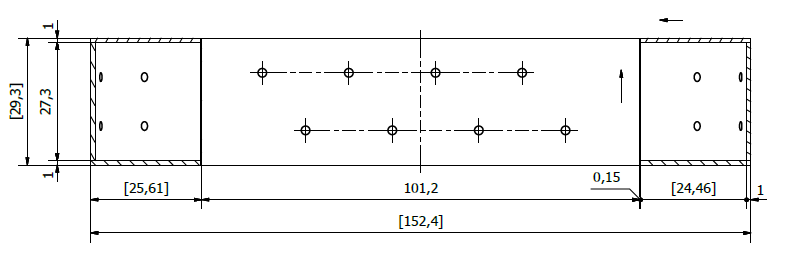
\includegraphics[width=\linewidth]{sections/skew_quad_q_det/figures/skew_quad_design/skew_quad_transversal_cross_section.png}} at (0,0);
    \node[red] at (6.0,2.1) {layers};
    \node[red, rotate=90] at (4.3,0) {turns};
    \draw[red, very thick, dashed] (0.47,-0.95) -- (0.47,2.4); 
    \node[red, scale=0.8] at (1.9,2.1) {coil symmetry};
    \draw[black, very thick, ->] (-4.3,2.1) -- (-4.8,1.8); 
    \node[black, scale=0.8] at (-3.0,2.1) {ground insulation};
    \end{tikzpicture}
    \caption{The transversal cross-section of one coil of a skew quadrupole~\cite{marco_prioli_mails}.}
    \label{fig:skew_quad_transversal_cross_section}
\end{figure}

As shown in Fig.~\ref{fig:winding_arrangement_cross_section}, each coil has 29 turns in each of its 26 layers. In total, the number of windings per coil is 754~\cite{marco_prioli_mails, hl_lhc_tech_design_report_v01}.

\begin{figure}[H]
\centering
    \begin{tikzpicture}
        \begin{axis}[
          width=0.5\linewidth, 
          height=0.5\linewidth,
          xtick={0.0, 24.46},
          ytick={0.0, 27.30},
          xlabel={$x,~\text{mm}~\text{(layers direction)}$},
          ylabel={$y,~\text{mm}~\text{(turns direction)}$},
          xmajorgrids=true,
          ymajorgrids=true,
          xmin=-5.0,
          xmax=29.47,
          ymin=-5.0,
          ymax=32.29,
          ]
          \addplot[blue, only marks, mark size=1pt] table[x=x,y=y,col sep=comma] {sections/skew_quad_q_det/figures/skew_quad_design/winding_location_cross_section.csv};
        \end{axis}
        \draw[scale=0.172, red, very thick, dashed] (2.5,2) -- (2.5,33.0); 
        \node[red, scale=0.8] at (1.9,5.6) {coil symmetry};
        
    \end{tikzpicture}
    \caption{Location of the windings in the cross-section of a half-coil.}
    \label{fig:winding_arrangement_cross_section}
\end{figure}

The winding scheme is shown in Fig.~\ref{fig:winding_scheme_cross_section}. The winding~1 is placed at the bottom left of the 2D cross-section. The last winding number 754 is placed further in the \textit{x}-direction. The \nth{2} half of the coil is a~mirror reflection of the presented winding scheme.

\begin{figure}[H]
\centering
    \begin{tikzpicture}
        \begin{axis}[
          width=0.5\linewidth, 
          height=0.5\linewidth,
          xtick={0.0, 24.46},
          ytick={0.0, 27.30},
          xlabel={$x,~\text{mm}~\text{(layers direction)}$},
          ylabel={$y,~\text{mm}~\text{(turns direction)}$},
          xmajorgrids=true,
          ymajorgrids=true,
          xmin=-5.0,
          xmax=29.47,
          ymin=-5.0,
          ymax=32.29,
          ]
        \end{axis}
        \foreach \t in {0.471, 2.353,...,24}
            \draw[scale=0.172, blue, thick, ->] (\t+5.35,5.0) -- (\t+5.35,26.819+3.3); 
        \foreach \t in {1.412, 3.294,...,25}
            \draw[scale=0.172, red, thick, ->] (\t+5.35,26.819+3.3) -- (\t+5.35,5.0);
        \draw[scale=0.172, red, very thick, dashed] (2.5,2) -- (2.5,33.0); 
        \node[red, scale=0.8] at (1.9,5.6) {coil symmetry};
        \filldraw[scale=0.172, black] (0.471+5.35,5.0) circle (10pt);
        \node[black, scale=0.8] at (1.2,0.5) {winding 1};
        \filldraw[scale=0.172, black] (23.996+5.35,5.0) circle (10pt);
        \node[black, scale=0.8] at (5.0,0.5) {winding 754};
        
    \end{tikzpicture}
    \caption{Winding scheme of a single coil of the skew quadrupole.}
    \label{fig:winding_scheme_cross_section}
\end{figure}

The general parameters of the skew quadrupole are summarised in Table~\ref{table:skew_quad_params_table}. In the given magnet, there is only one aperture in which a particle beam travels through. Four coils of the magnet are connected in series and powered by a single power converter. It is interesting to mention that the coil length of only one coil is more than 800~m which is a very large number for thermal quench simulations, as mentioned in Section~\ref{section: 1D_quench_propagation_conclusions}. The operating current of the skew quadrupole is $I=182~\text{A}$.

\begin{table}[H]
    \caption{Geometrical parameters for skew quadrupole \cite{marco_prioli_mails, hl_lhc_tech_design_report_v01}} 
    \vspace{-1.em} 
    \fontsize{10}{10}
    \selectfont 
    \renewcommand{\arraystretch}{1.5}
    \begin{center}
    \begin{tabular}{ ccc }  
    \hline
    parameter & value & unit \\
    \hline
    number of apertures & 1 & [-] \\
    number of circuits & 1 & [-] \\
    aperture size & 150 & [mm]\\
    coil length & 841 & [m] \\
    operating current & 182 & [A] \\
    \hline 
    \end{tabular}
    \end{center}  
     \label{table:skew_quad_params_table} 
 \end{table}

\section{Quench Measurements}
\label{section:quench_measurements}

During the measurements, the spot heater was attached to the external ground insulation of one of the four coils of the magnet. The heater contact area of 4~$\text{mm}^2$ was centered at the layer 13 on the aperture side of the magnet, as presented in Fig.~\ref{fig:spot_heater_placement}.

\begin{figure}[H]
\centering
    \begin{tikzpicture}
        \begin{axis}[
          width=0.5\linewidth, 
          height=0.5\linewidth,
          xtick={0.0, 24.46},
          ytick={0.0, 27.30},
          xlabel={$x,~\text{mm}~\text{(layers direction)}$},
          ylabel={$y,~\text{mm}~\text{(turns direction)}$},
          xmajorgrids=true,
          ymajorgrids=true,
          xmin=-5.0,
          xmax=29.47,
          ymin=-5.0,
          ymax=32.29,
          ]
          \addplot[blue, only marks, mark size=1pt] table[x=x,y=y,col sep=comma] {sections/skew_quad_q_det/figures/skew_quad_design/winding_location_cross_section.csv};
        \end{axis}
        \draw[scale=0.172, black, ultra thick] (3.0,4.5) -- (32.0,4.5); 
        \node[black, scale=0.8] at (4.9,0.5) {ground insulation};
        \filldraw[scale=0.172, red] (0.471+5.35+0.941*12,3.7) circle (13pt);
        \node[red, scale=0.8] at (3.0,0.3) {spot heater};

    \end{tikzpicture}
    \caption{Location of the spot heater with respect to the coil cross-section~\cite{marco_prioli_mails}.}
    \label{fig:spot_heater_placement}
\end{figure}

The coil is quenched due to the heat generated in the spot-heater. The heat is a~result of a~current discharge in the~\nth{1} order RC-circuit as shown in Fig.~\ref{fig:spot_heater_capacitor_discharge}. Its capacitance was equal to $C=14~\text{mF}$.

\begin{figure}[H]
	\centering
	\begin{tikzpicture}[american resistors, scale = 0.8] 
	\draw[semithick] 
	(-2,0)
	to[C,l^=$C$] (-2,2) -- (2,2);
	\draw[semithick] 
	(-2,0) -- (2,0)
	to[R,l^=$R_\text{spot heater}$] (2,2);
	\draw[semithick, red] (3,-0.5) -- (3,2.5) -- (6,2.5) -- (6,-0.5) -- (3,-0.5);
	\node[red, scale=0.8] at (4.5,1) {magnet domain};
	\end{tikzpicture}
	\caption{Schematic of heating the magnet by means of a spot heater.}
	\label{fig:spot_heater_capacitor_discharge}
\end{figure}

The spot heater resistance is calculated as
\begin{equation}
    R_\text{spot heater} = \frac{\tau}{C},
\end{equation}
where $\tau$ -- time constant, $C$ -- capacitance. The electric energy of the capacitor is directly dissipated in the spot-heater. Therefore, the power dissipation at the spot heater is calculated as
\begin{equation}
    P(t)_\text{spot heater} = -P(t)_\text{capacitor} = -\frac{1}{\text{dt}} (E_\text{C}) = -\frac{1}{\text{dt}} (\frac{1}{2} \text{C}V_\text{C}^2),
    \label{eqn:power_dissipation}
\end{equation}
where $V_\text{C}$ -- voltage across the capacitor, $E_\text{C}$ -- energy stored in the capacitor, $P(t)$ -- power being a function of time. Figure~\ref{fig:capacitor_discharge} presents the measured drop of a~capacitive voltage when the capacitor was discharging. The same Figure also presents the~deduced power dissipation at the~spot heater based on~(\ref{eqn:power_dissipation}). The sampling frequency of the measurements was equal to $f=5000~\text{Hz}$. Based on the power curve in Fig.~\ref{fig:capacitor_discharge}, one can notice that most of energy was transmitted to the coil during the first $t=5~\text{ms}$ and the capacitor was fully discharged at $t=10~\text{ms}$. The bath temperature of the coil during the measurements was $T_0=4.3~\text{K}$.

\begin{figure}[H]
\centering
\begin{tikzpicture}
\pgfplotsset{
    width=0.7\linewidth, 
    height = 4.0cm,
    compat=1.3,
    xmin=0, xmax=20.0,
    xticklabel style={/pgf/number format/fixed},
    xtick={0,5,10,15,20},
    legend pos=north east
}
\begin{axis}[
  axis y line*=left,
  ymin=0, ymax=20,
  xlabel={Time, ms},
  ylabel={$V_\text{C}$,~V},
]
\addplot[smooth, red] table[x=time,y=v_capacitor,col sep=comma] {sections/skew_quad_q_det/figures/measurements/capacitor_discharge.csv};
\label{plot_voltage_discharge_capacitor}
\end{axis}

\begin{axis}[
  axis y line*=right,
  axis x line=none,
  ymin=0, ymax=2200,
  ylabel={$P_\text{spot heater}$, W},
]
\addplot[smooth, blue] table[x=time,y=p_capacitor,col sep=comma] {sections/skew_quad_q_det/figures/measurements/capacitor_discharge.csv}; 
\label{plot_power_deposition_resitor}

\addlegendentry{$P_\text{spot heater}$}
\addlegendimage{/pgfplots/refstyle=plot_voltage_discharge_capacitor}\addlegendentry{$V_\text{C}$}

\end{axis}
\end{tikzpicture}
\caption{Voltage drop across the capacitor and heating power curve at the spot heater.}
\label{fig:capacitor_discharge}
\end{figure}

With the shape of the voltage drop, the time constant and spot heater resistance were deduced, as shown in Table~\ref{table:rc_circuit_characteristics}. Moreover, the entire capacitive energy deposited in the~magnet was approximately equal to $E_\text{C}=2.5~\text{J}$.

 \begin{table}[H]
    \caption{RC heating circuit characteristics.} 
    \vspace{-1.em} 
    \fontsize{10}{10}
    \selectfont 
    \renewcommand{\arraystretch}{1.5}
    \begin{center}
        \begin{tabular}{ ccc } 
        \hline
        parameter & value & unit \\
        \hline
        $\tau$ & 3.5 & [ms] \\
        $R_\text{spot heater}$ & 0.25 & [\textOmega] \\
        $E_\text{C}$ & 2.5 & [J] \\
        \hline 
        \end{tabular}
    \end{center}  
     \label{table:rc_circuit_characteristics} 
 \end{table}

The electrical circuit schematic of the skew quadrupole is presented in Fig.~\ref{fig:skew_quad_electrical_scheme}. Each coil is characterised by the same self-inductance $L_\text{coil}$. Since all coils are connected in series, it is possible to include their mutual inductance in the self-inductance. During the measurements, the heat was not transmitted to other coils of the skew quadrupole, i.e. only one coil out of four quenched. $R_\text{coil}$ in Fig.~\ref{fig:skew_quad_electrical_scheme} represents the internal resistance of the coil where the spot heater was placed. When the skew quadrupole is in the superconducting state, $R_\text{coil}=0$. After the quench is provoked by depositing heat through the spot heater, $R_\text{coil}$ represented by a varying resistance starts increasing. In order to detect a quench, the voltages $V_1$ and $V_2$ are compared. If their difference exceeds a threshold value, $V_\text{th}$ during a certain period of time, the quench is detected. The time after which the quench is detected after exceeding the threshold $V_\text{th}$ is described as the validation time, $t_\text{validation}$. When the quench is detected, the switch $\text{s}_\text{power}$ closes and cuts off the power converter whereas the switch $\text{s}_\text{dump}$ opens leading to the discharge of the energy stored in the circuit in the dump resistor $R_\text{dump}$. The schematic in Fig.~\ref{fig:skew_quad_electrical_scheme} neither includes the protection devices of the energy extraction system nor the ones of the power converter as they do not affect the quench protection study in this thesis.

\begin{figure}[H]
	\centering
	\begin{tikzpicture}[american currents, american inductors, american resistors, scale = 0.7] 
	\draw[semithick] 
	(0,-0.5) -- (0,2)
	to[vL,l^=$L_\text{coil}$, o-] (2,2)
	to[vL,l^=$L_\text{coil}$, -o] (4,2)
	to[vL,l^=$L_\text{coil}$] (6,2)
	to[vL,l^=$L_\text{coil}$] (8,2)
	to[vR,l^=$R_\text{coil}$, -o] (10,2) -- (10,-0.5)
	(0,-0.5) to[I, l_=$P_\text{converter}$]  (5,-0.5)
	(5,-0.5) to[R,l^=$R_\text{dump}$] (10,-0.5);
	
	\draw[semithick]
	(1,-0.5) -- (1,0.5)
	to[closing switch, l=$\text{s}_\text{power}$] (4,0.5) -- (4,-0.5);
	
	\draw[semithick]
	(6,-0.5) -- (6,0.5)
	to[opening switch, l=$\text{s}_\text{dump}$] (9,0.5) -- (9,-0.5);
	
	\draw[semithick]
	(4,2) -- (4,4)
	to[voltmeter, l=$V_1$] (10,4) -- (10,2);
    \draw[semithick]
    (0,2) -- (0,4)
    to[voltmeter, l=$V_2$] (4,4);

    \draw[semithick]
    (0,-0.5) -- (0,-0.5) node[ground]{}; 
	\end{tikzpicture}
	\caption{Circuit schematic of the skew quadrupole with marked directions of closing/opening switches when a quench is detected.}
	\label{fig:skew_quad_electrical_scheme}
\end{figure}

The quench detection system parameters are presented in Table~\ref{table:qds_characteristics}. The voltage threshold $V_\text{th}$ should be exceeded during the validation time $t_\text{validation}=20~\text{ms}$ in order to disconnect the power converter.

\begin{table}[H]
    \caption{Characteristics of the quench detection system.} 
    \vspace{-1.em} 
    \fontsize{10}{10}
    \selectfont 
    \renewcommand{\arraystretch}{1.5}
    \begin{center}
        \begin{tabular}{ ccc } 
        \hline
        parameter & value & unit \\
        \hline
        $V_\text{th}$ & 0.2 & [V] \\
        $t_\text{validation}$ & 20 & [ms] \\
        \hline 
        \end{tabular}
    \end{center}  
     \label{table:qds_characteristics} 
\end{table}

After the quench is detected, the circuit is represented, as shown in Fig.~\ref{fig:skew_quad_discharge_electrical_scheme}. The total magnet inductance $L_\text{magnet}$ is calculated as~\cite{marco_prioli_mails}
\begin{equation}
    L_\text{magnet} = 4 L_\text{coil} + 8 M_\text{a} + 4 M_\text{b},
\end{equation}
where $M_\text{a}$ -- mutual inductance between adjacent coils, $M_\text{b}$ -- mutual inductance between opposite coils. The initial discharge current $I_0$ is equal to the operating current of the magnet during the measurements.

\begin{figure}[H]
	\centering
	\begin{tikzpicture}[american currents, american inductors, american resistors, scale = 0.8] 
	\draw[semithick] 
	(0,0) -- (0,2)
	to[vL,l^=$L_\text{magnet}$, i_=$I_0$] (6,2)
	to[vR,l^=$R_\text{coil}$] (6,0)
	to[R,l^=$R_\text{dump}$] (0,0);
    \draw[semithick]
    (0,0) -- (0,0) node[ground]{}; 
	\end{tikzpicture}
	\caption{Simplified circuit scheme of the skew quadrupole after the quench is detected.}
	\label{fig:skew_quad_discharge_electrical_scheme}
\end{figure}

If the magnet is self-protected, $R_\text{dump}=0$. The dump resistance of the energy extraction system equals $R_\text{dump}=1.557$~\textOmega~\cite{marco_prioli_mails}. One should remember that $\tau$ is not constant during the discharge due to the nonlinear inductance as a function of current and increasing $R_\text{coil}$ as the quench propagates. The~time constant of the circuit is calculated as 
\begin{equation}
    \tau = \frac{L_\text{magnet}}{R_\text{coil}+R_\text{dump}}.
    \label{eqn:variable_time_constant}
\end{equation}

The quench measurements were conducted for $I=86~\text{A}$ which is a lower value than the designed nominal operating current of the skew quadrupole. As presented in Fig.~\ref{fig:skew_quad_discharge_before_quench_detection}, the quench resistive voltage reaches the threshold value for the quench detection system at $t=130~\text{ms}$. The quench is detected at $t=150~\text{ms}$.~\cite{marco_prioli_mails}

\begin{figure}[H]
\centering
\begin{tikzpicture}
\pgfplotsset{
    height=4.0cm,
    width=0.7\linewidth, 
    compat=1.3,
    scaled x ticks=base 10:3,
    xmin=0, xmax=0.15,
    legend pos=outer north east
}
\begin{axis}[
  axis y line*=left,
  ymin=0, ymax=0.35,
  xlabel={$t$, s},
  ylabel={$V_\text{res}$, V},
]
\addplot[smooth, red] table[x=Time,y=Resistive_Voltage,col sep=comma] {sections/skew_quad_q_det/figures/measurements/current_voltage_quench_detection.csv}; 
\label{plot_resistive_voltage_rise_quench_detection}
\addplot[smooth, black, dashed] table[x=Time,y=QDS_v_threshold,col sep=comma] {sections/skew_quad_q_det/figures/measurements/current_voltage_quench_detection.csv};
\label{plot_resistive_voltage_qds_threshold}
\end{axis}

\begin{axis}[
  axis y line*=right,
  axis x line=none,
  ymin=0, ymax=100,
  ylabel={$I$, A},
  legend pos=south west
]
\addplot[smooth, blue] table[x=Time,y=Current,col sep=comma] {sections/skew_quad_q_det/figures/measurements/current_voltage_quench_detection.csv}; 
\label{plot_current_constant_quench_detection}
\addlegendentry{$I$}
\addlegendimage{/pgfplots/refstyle=plot_resistive_voltage_qds_threshold}\addlegendentry{$V_\text{th}$}
\addlegendimage{/pgfplots/refstyle=plot_resistive_voltage_rise_quench_detection}\addlegendentry{$V_\text{res}$}

\end{axis}
\end{tikzpicture}
\caption{Resistive voltage rise as a function of time at constant current before the quench detection~\cite{marco_prioli_mails}.}
\label{fig:skew_quad_discharge_before_quench_detection}
\end{figure}

Figure~\ref{fig:skew_quad_discharge} presents the current profile as well as the change of resistive voltage across the~magnet during the discharge of the skew quadrupole. The resistive voltage $V_\text{res}$ is a function of coil resistance $R_\text{coil}$ and the value of current in the circuit. Until $t=1.5~\text{s}$, the rise of voltage up to approximately 16~V is observed due to the increase of coil resistance mainly because of a turn-to-turn propagation. After this time, the voltage drops down because the~current decreases rapidly in the circuit. The smooth shape of the current curve indicates that the quench back did not occur during the discharge which can be explained by a~relatively long discharge time. The quench measurements ended at $t=9~\text{s}$.

\begin{figure}[H]
\centering
\begin{tikzpicture}
\pgfplotsset{
    width=0.7\linewidth, 
    height = 4.0cm,
    compat=1.3,
    scaled x ticks=base 10:0,
    xmin=0, xmax=9,
    legend pos= north east
}
\begin{axis}[
  axis y line*=left,
  ymin=0, ymax=20,
  xlabel={$t$, s},
  ylabel={$V_\text{res}$, V},
]
\addplot[smooth, red] table[x=Time,y=Resistive_Voltage,col sep=comma] {sections/skew_quad_q_det/figures/measurements/current_voltage_discharge.csv}; 
\label{plot_resistive_voltage_entire_discharge_skew_quad}
\end{axis}
\begin{axis}[
  axis y line*=right,
  axis x line=none,
  ymin=0, ymax=100,
  ylabel={$I$, A}
]
\addplot[smooth, blue] table[x=Time,y=Current,col sep=comma] {sections/skew_quad_q_det/figures/measurements/current_voltage_discharge.csv}; 
\label{plot_current_entire_discharge_skew_quad}
\addlegendentry{$I$}
\addlegendimage{/pgfplots/refstyle=plot_resistive_voltage_entire_discharge_skew_quad}\addlegendentry{$V_\text{res}$}
\end{axis}
\end{tikzpicture}
\caption{Current and Resistive Voltage change during the discharge of skew quadrupole~\cite{marco_prioli_mails}.}
\label{fig:skew_quad_discharge}
\end{figure}



\section{Magnetic Map of Skew Quadrupole}
\label{section: magnetic_map_skew_quad}

\subsection{Material Properties and Geometry}

Figure~\ref{fig:skew_quad_geometry_ansys} presents a cross-section of the skew quadrupole used for a magnetic analysis. The iron yoke, the coil, and the remaining parts of the model considered as air are marked in red, blue, and violet respectively. The~magnet cross-section has three axes of symmetry. Therefore, only one-eighth of the skew quadrupole is simulated.  

\begin{figure}[H]
    \centering
    \begin{tikzpicture}[scale=0.8]
    \node[scale=0.8] at (0,0) {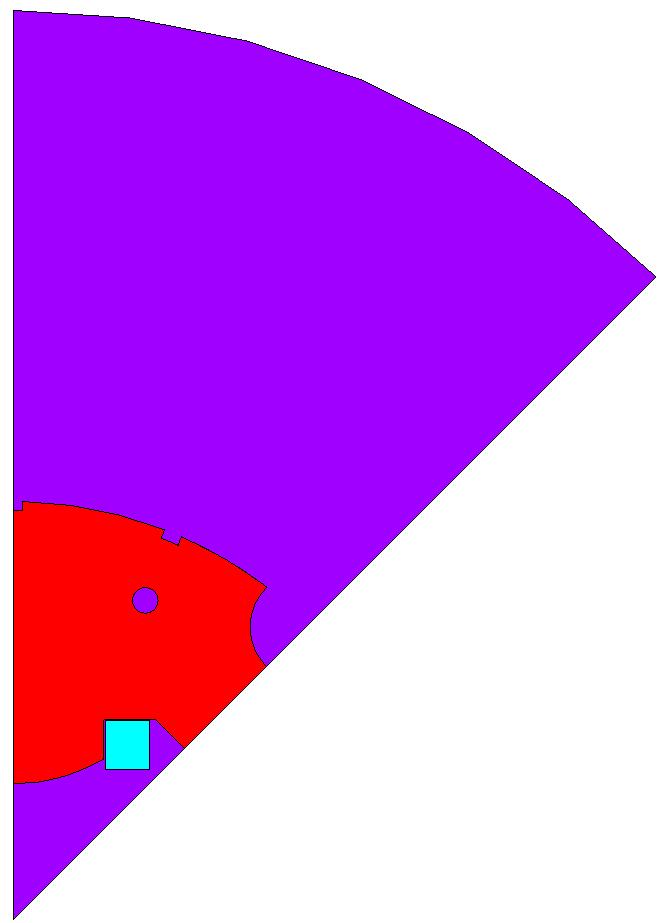
\includegraphics[width=.3\textwidth]{sections/skew_quad_q_det/figures/magnetic_map/skew_quad_geometry.png}};

    \draw[black, thick, ->] (2.5,0) -- (-1.1,0);
    \draw[black, thick, ->] (2.5,-0.95) -- (-1.32,-0.95);
    \draw[black, thick, ->] (2.5,-1.5) -- (-1,-1.5);
    \draw[black, thick, ->] (2.5,-2) -- (-1.4,-2);
    \draw[black, thick, ->] (2.5,-2.5) -- (-1.8,-2.5);
    
    \draw[red, dashed] (-2.35,-3.3) -- (2.5,-3.3);
    \draw[red, dashed] (-2.3,-3.3) -- (-2.3,3.3);
    \draw[red, dashed] (-2.35,-3.45) -- (2.8,1.67);
    \node[red, scale=0.8] at (3.5,1.9) {axes of symmetry};
    
    \node[black, scale=0.8] at (3.5,0) {air external};
    \node[black, scale=0.8] at (3.5,-0.95) {air hole};
    \node[black, scale=0.8] at (3.5,-1.5) {iron yoke};
    \node[black, scale=0.8] at (3.5,-2) {coil};
    \node[black, scale=0.8] at (3.5,-2.5) {air internal};

    \end{tikzpicture}
    \caption{The \nth{8} part of the skew quadrupole cross-section with specified component names.}
    \label{fig:skew_quad_geometry_ansys}
\end{figure}

The~coil cross-section is homogenised magnetically and electrically, i.e. there is no distinction between the insulation and the strand composite. In the magnetic analysis of the~skew quadrupole, it is assumed that the magnet is infinitely long. This assumption allows for considering this case as a plane 2D problem. The areas considered as air and the~coil are characterised by the magnetic relative permeability equal to one. The iron yoke is characterised by a~non-linear B-H curve, as presented in Fig.~\ref{fig:b_h_curve}. 

\begin{figure}[H]
    \centering
    \begin{tikzpicture}
        \begin{axis}[
          width=0.7\linewidth, 
          height = 4.0cm,
          xlabel={$H,~\text{A/m}$},
          ylabel={$B,~\text{T}$},
          ymax=3.0,
          ]
          \addplot[smooth, blue] table[x=h,y=b,col sep=comma] {sections/skew_quad_q_det/figures/magnetic_map/bh_curve.csv}; 
    \end{axis}
    \end{tikzpicture}
    \caption{B-H curve of an iron yoke of the skew quadrupole.}
    \label{fig:b_h_curve}
\end{figure}


\subsection{Mesh, Initial and Boundary Conditions}

The meshed geometry is illustrated in Fig~\ref{fig:skew_quad_magnetic_mesh_ansys}. The element PLANE233 is used for the analysis. It is a 2-D element for simulating 2D planar and axisymmetric magnetic fields. The element is defined by 8 nodes~\cite{ansys_element_manual}.

\begin{figure}[H]
    \centering
    \begin{tikzpicture}[scale=0.9]
    \node[scale=0.9] at (0,0) {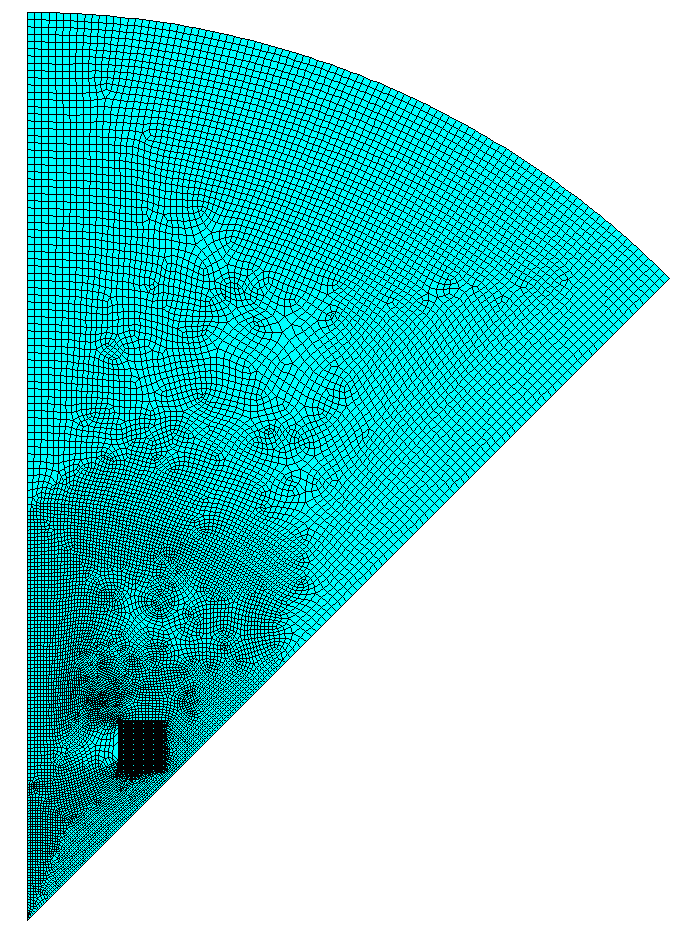
\includegraphics[width=.3\textwidth]{sections/skew_quad_q_det/figures/magnetic_map/skew_quad_mesh.png}};
    \node[scale=0.9] at (5,0) {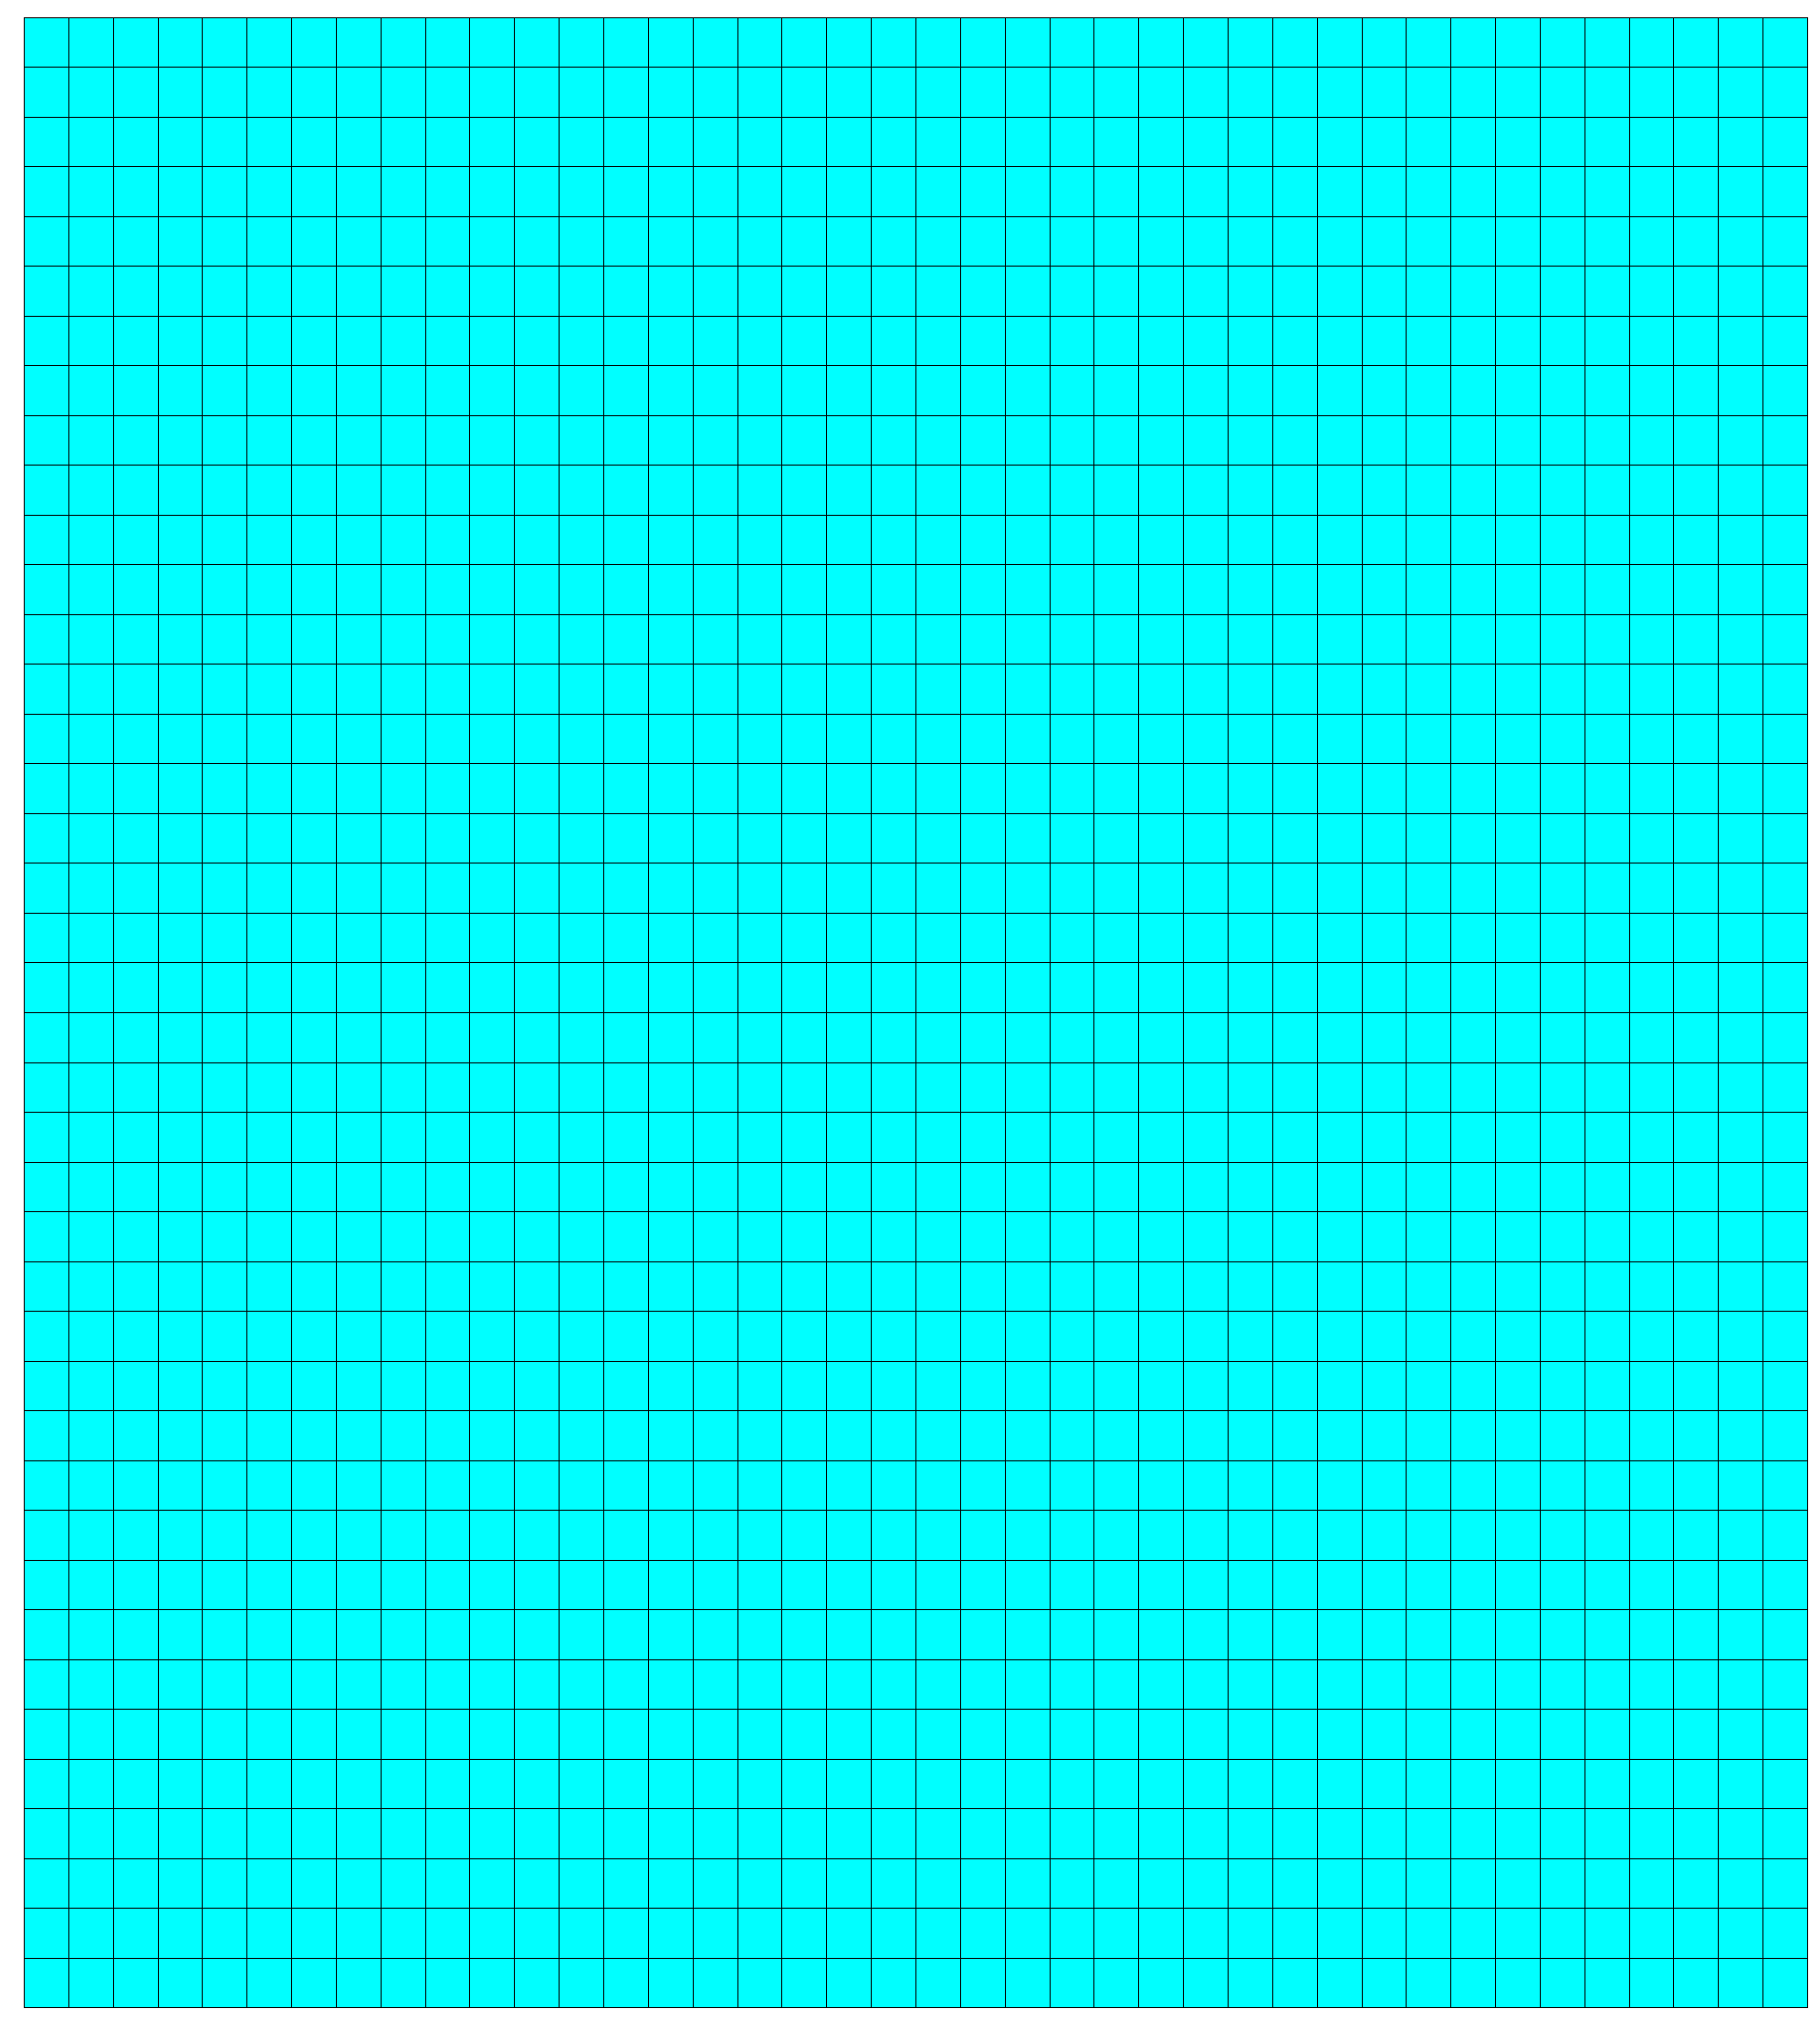
\includegraphics[width=.25\textwidth]{sections/skew_quad_q_det/figures/magnetic_map/skew_quad_mesh_coil.png}};
    \draw[red, very thick, dashed] (-2.3,-3.1) -- (-2.3,3.1);
    \node[red, scale=0.8] at (-3,2) {$A_\text{z}=0$};
    
    \draw[black, very thick, ->] (-0.9,-1.9) -- (3.0,0);
    \node[black, scale=0.8] at (5,2.5) {Mesh in the coil};
    
    \draw[scale=1] (-3.5,1-1) circle (0.1cm);
    \draw[black, ->, scale=1] (-3.5,1-1) -- (-3.5,1.5-1);
    \draw[black, ->, scale=1] (-3.5,1-1) -- (-3,1-1);
    \node[scale = 0.8] at (-3.75,0.8-1) {$\vec{z}$};
    \node[scale = 0.8] at (-2.9,1.2-1) {$\vec{x}$};
    \node[scale = 0.8] at (-3.7,1.65-1) {$\vec{y}$};
    
    \end{tikzpicture}
    \caption{The \nth{8} part of the skew quadrupole cross-section.}
    \label{fig:skew_quad_magnetic_mesh_ansys}
\end{figure}

For the requirements of the given analysis, the degrees of freedom only related to the~magnetic vector potential $A_\text{z}$ are used. In order to take into consideration the symmetry condition, the~magnetic vector potential $A_\text{z}$ is set to zero on the left side of the geometry. It means that the directional magnetic field $B_\text{x}$ is equal to zero on the left side marked in red. On the other side of the symmetry axis, it is assumed by default in ANSYS APDL that the magnetic flux is perpendicular to the wall. As illustrated in Fig~\ref{fig:skew_quad_magnetic_mesh_ansys}, the mesh is refined inside of the coil. There are 40 elements placed on each side of a rectangular area. The element size in the remaining components of the model is depicted in Table~\ref{table:mesh_characteristics_magnetic_ansys}.

\begin{table}[H]
    \caption{Mesh size characteristics of the skew quadrupole.} 
    \vspace{-1.em} 
    \fontsize{10}{10}
    \selectfont 
    \renewcommand{\arraystretch}{1.5}
    \begin{center}
        \begin{tabular}{ ccc } 
        \hline
        area name & element size & unit \\
        \hline
        iron yoke & 2 & mm \\
        air internal & 1.5 & mm \\
        air external & 4 & mm \\
        air hole & 2 & mm \\
        \hline 
        \end{tabular}
    \end{center}  
     \label{table:mesh_characteristics_magnetic_ansys} 
\end{table}

The uniformly distributed current density is applied to the coil area calculated as
\begin{equation}
    J_\text{coil} = \frac{n_\text{windings}~I}{A_\text{coil}},
\end{equation}
where $n_\text{windings}$ -- number of windings, $I$ -- current in each winding, $A_\text{coil}$ -- cross-sectional area of the coil with the resin and insulation. 86 static analyses are conducted with current linearly rising from 1 up to 86~A. 

\subsection{Results and Magnetic Field Mapping in the Skew Quadrupole}

Two values of current are chosen for the comparison of the magnetic field distribution inside the cross-section of the skew quadrupole, as shown in Fig.~\ref{fig:skew_quad_magnetic_results_geometry_ansys}. As expected, one can observe that the magnetic field increases with the rise of current. Moreover, the difference in the magnetic field distribution at different current levels is a result of the non-linear magnetic properties of the iron yoke.

\begin{figure}[H]
    \centering
    \begin{tikzpicture}
    \node at (0,0) {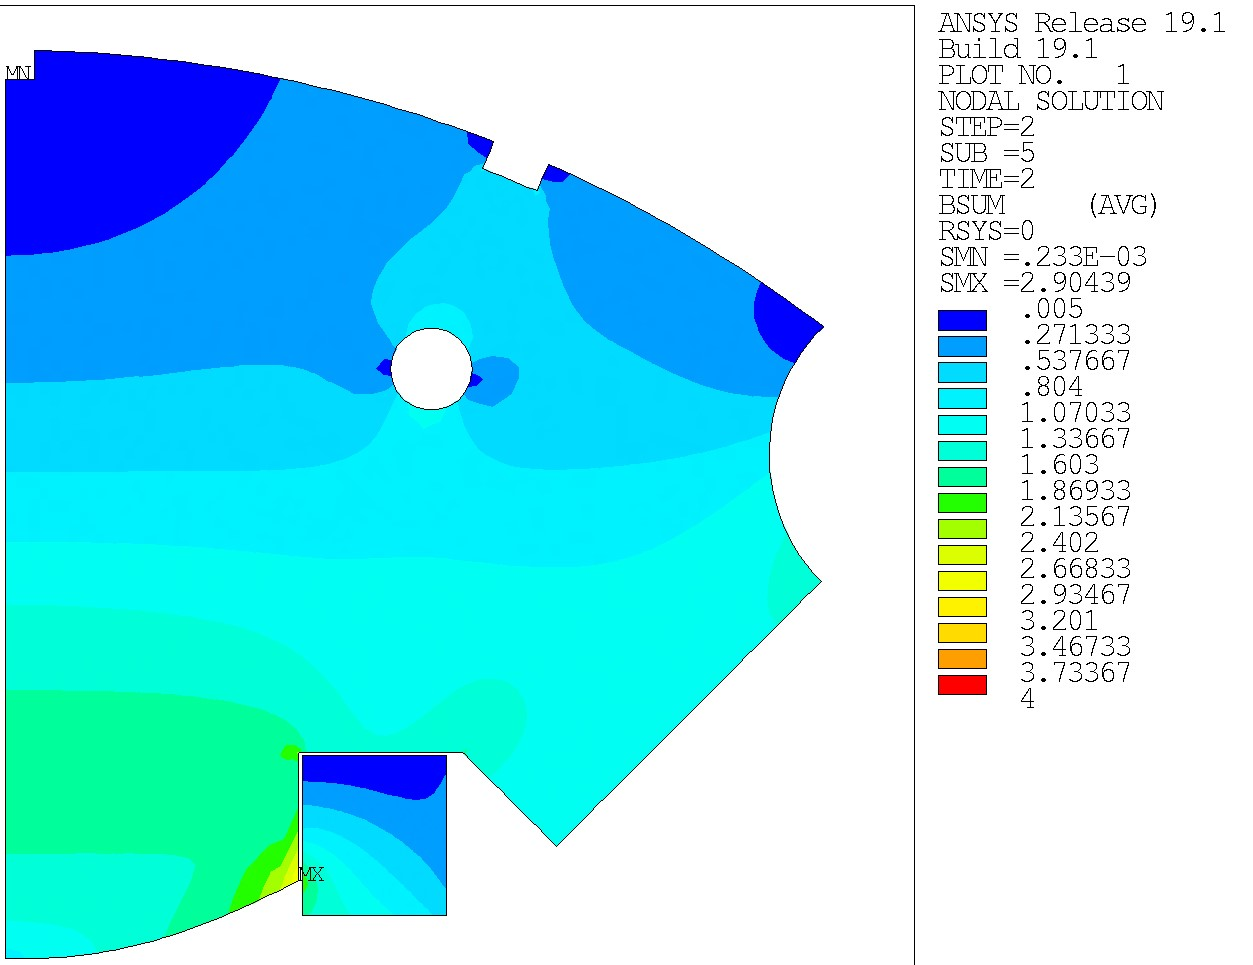
\includegraphics[width=.39\textwidth]{sections/skew_quad_q_det/figures/magnetic_map/peak_field_yoke_coil_current_40.jpg}};
    \node at (7.5,0) {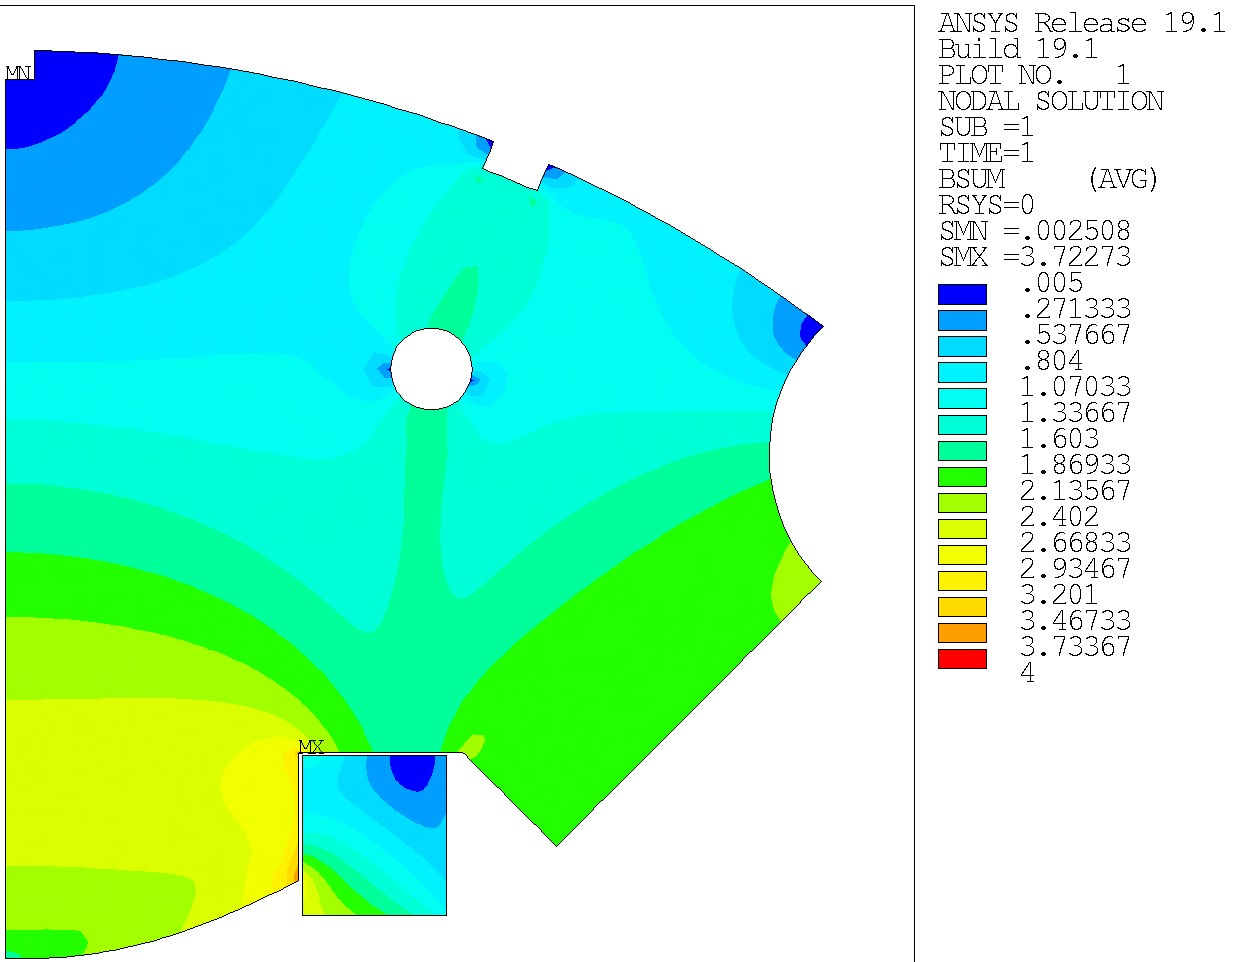
\includegraphics[width=.39\textwidth]{sections/skew_quad_q_det/figures/magnetic_map/peak_field_yoke_coil_current_86.jpg}};
    \end{tikzpicture}
    \caption{Magnetic field distribution in the coil and the iron yoke for $I=40~\text{A}$ (left) and $I=86~\text{A}$ (right).}
    \label{fig:skew_quad_magnetic_results_geometry_ansys}
\end{figure}

Figure~\ref{fig:skew_quad_magnetic_results_coil_ansys} presents the magnetic field distribution only in the coil for two values of transport current. In order to use the results from the coil for the quench velocity-based approach, the vector sum of the magnetic flux density is extracted at corner nodes of the coil elements. The magnetic field is linearly interpolated in the $(x,y)$-space for the current levels between the actually simulated values. 

\begin{figure}[H]
    \centering
    \begin{tikzpicture}
    \node at (0,0) {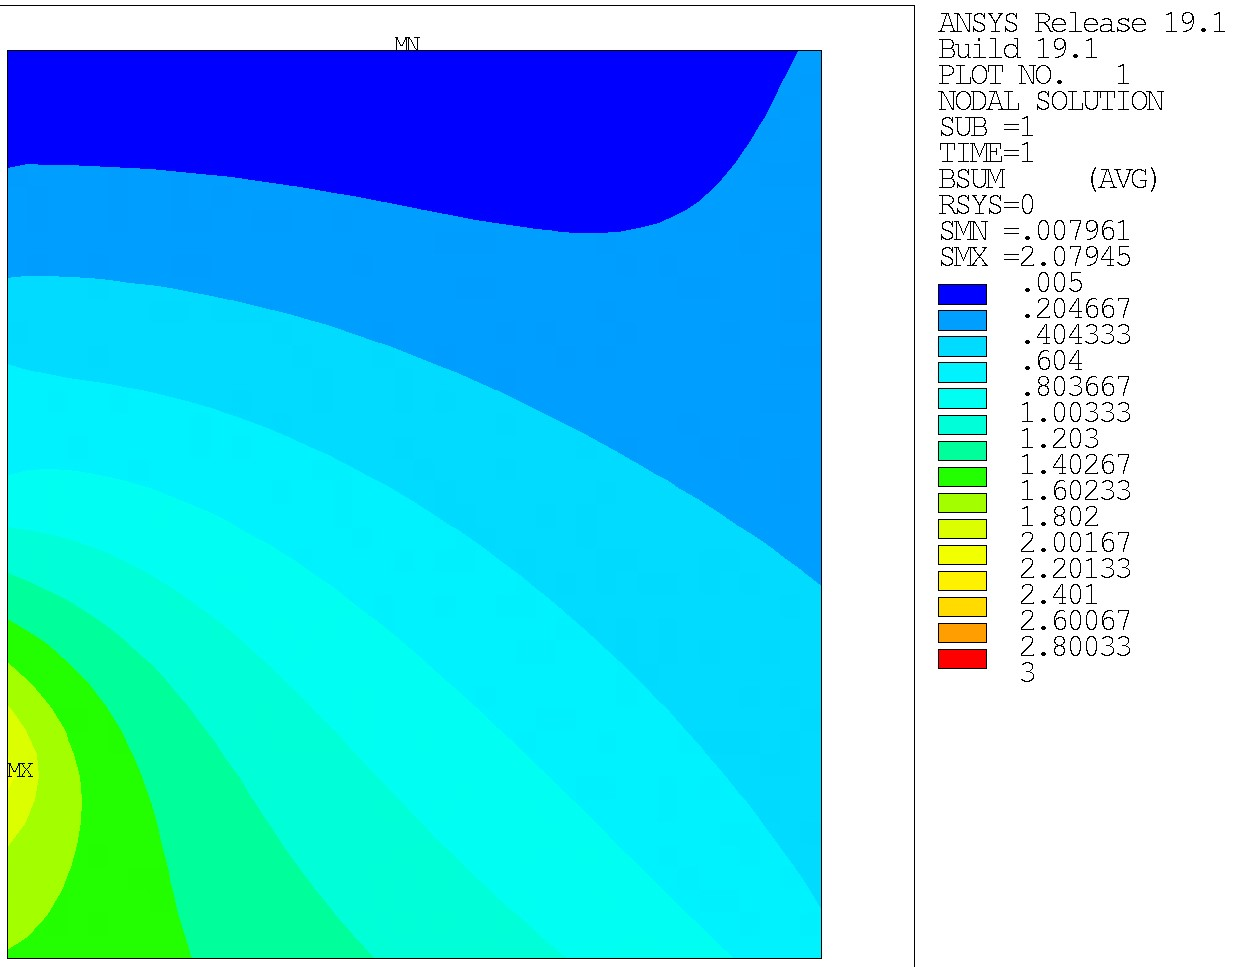
\includegraphics[width=.39\textwidth]{sections/skew_quad_q_det/figures/magnetic_map/peak_field_coil_current_40.jpg}};
    \node at (7.5,0) {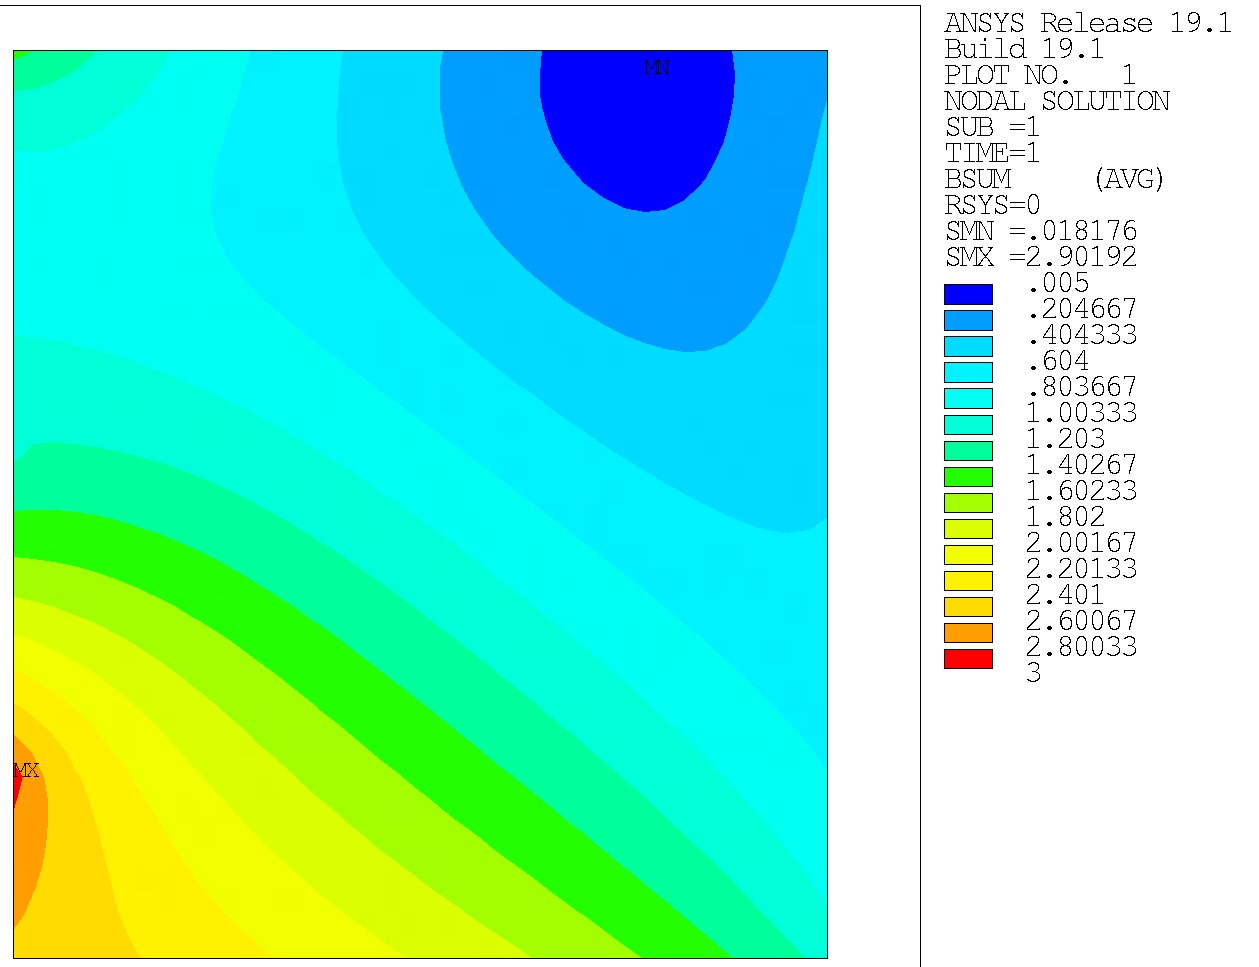
\includegraphics[width=.39\textwidth]{sections/skew_quad_q_det/figures/magnetic_map/peak_field_coil_current_86.jpg}};
    \end{tikzpicture}
    \caption{Magnetic field distribution in the coil for $I=40~\text{A}$ (left) and $I=86~\text{A}$ (right).}
    \label{fig:skew_quad_magnetic_results_coil_ansys}
\end{figure}

Figure~\ref{fig:skew_quad_magnetic_interpolation_coil_ansys} illustrates the magnetic field map applied to 754 windings for the nominal current of $I=86~\text{A}$. The central position of each winding is used to interpolate the magnetic field from the ANSYS results presented in Fig.~\ref{fig:skew_quad_magnetic_results_coil_ansys}. As current changes in time during the discharge process, the magnetic field of each winding varies with its position in the $(x,y)$-space.

\begin{figure}[H]
    \centering
    \begin{tikzpicture} [scale=0.8]
    
    \node[scale=0.8] at (0,0) {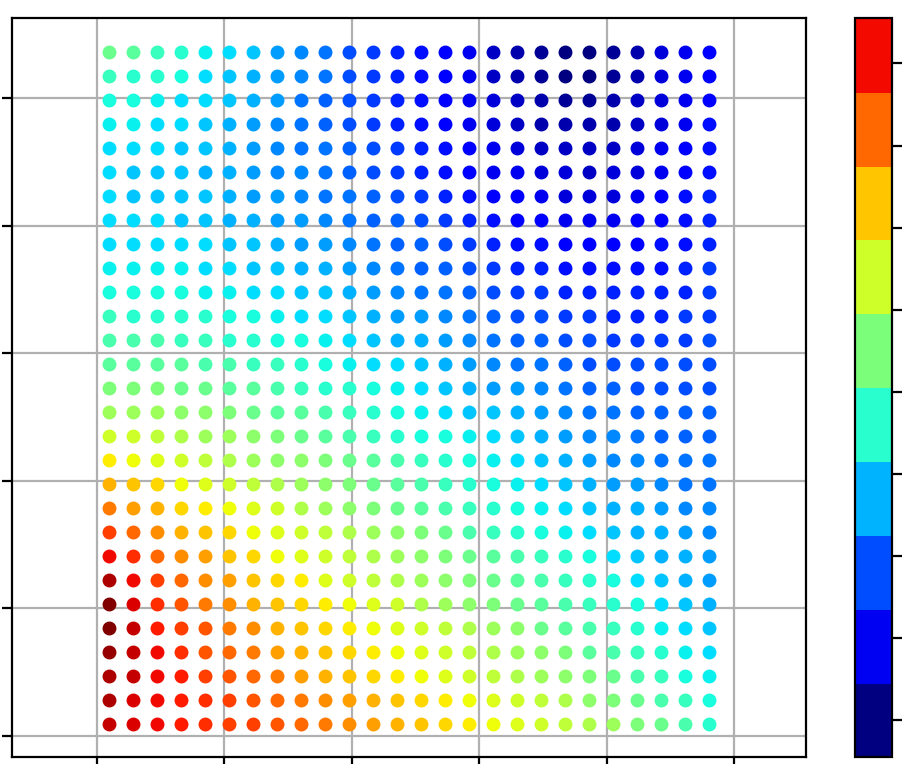
\includegraphics[width=.5\textwidth]{sections/skew_quad_q_det/figures/magnetic_map/Mag_field_distribution.png}};
    
    \node[black, scale=0.8] at (-3,-3.5) {0};
    \node[black, scale=0.8] at (-4.1,-2.95) {0};
    \node[black, scale=0.8] at (2.35,-3.6) {25};
    \node[black, scale=0.8] at (-4.1,2.45) {25};
    
    \node[black, scale=0.8] at (4.35,-2.82) {0.039};
    \node[black, scale=0.8] at (4.35,-2.2) {0.336};
    \node[black, scale=0.8] at (4.35,-1.5) {0.634};
    \node[black, scale=0.8] at (4.35,-0.8) {0.931};
    \node[black, scale=0.8] at (4.35,-0.1) {1.229};
    \node[black, scale=0.8] at (4.35,0.6) {1.526};
    \node[black, scale=0.8] at (4.35,1.3) {1.824};
    \node[black, scale=0.8] at (4.35,2) {1.121};
    \node[black, scale=0.8] at (4.35,2.7) {2.419};
    
    \node[black, scale=0.8] at (-0.225,-4) {$x$, mm (layers direction)};
    \node[black, rotate=90, scale=0.8] at (-4.75,0) {$y$, mm (layers direction)};
    \node[black, rotate=90, scale=0.8] at (5.3,0) {Magnetic field, T};

    \end{tikzpicture}
    \caption{Magnetic field distribution in the coil at $I=86~\text{A}$ applied separately to each winding.}
    \label{fig:skew_quad_magnetic_interpolation_coil_ansys}
\end{figure}

It is important to emphasise that ANSYS APDL allows for creating the material properties only as a function of a single-dependent variable (in this case temperature). It is not possible to include the dependence of material properties on the magnetic field in a relatively simple manner in this tool. The only possible method to add an additional variable in the repository of the material properties is to replace the repository at a certain moment of a transient simulation. The update of material properties is conducted at the communication time windows $t_\text{com}$ at which Python communicates with ANSYS to update the quench position in the coil. Since the update of the material properties is a time-consuming process, it is not recommended to perform it at each communication time window $t_\text{com}$ when hundreds of windings are modelled.

\section{Quench Velocity Map of Skew Quadrupole}

In order to conduct a quench velocity-based analysis with multiple strands, one should estimate the quench velocity for a varying values of magnetic field that can be found in the magnet. In the previous section, it was concluded that the maximum magnetic field in the skew quadrupole equals $B=3~\text{T}$ and occurs at the initial value of current, $I=86~\text{A}$. Moreover, as the current drops during the discharge, the quench velocity should also decrease because of the lower amount of energy deposited in the coil. Therefore, there are two main variables that have a direct impact on the quench velocity: 
\begin{itemize}
    \item magnetic field,
    \item current.
\end{itemize}
These two parameters are examined in 1D standard simulations with geometries of a relatively short length. 

\subsubsection{Adjustment of Insulation Layer}




\subsubsection{Quench Velocity Map}

\begin{figure}[H]
\centering
    \begin{tikzpicture}
        \begin{axis}[
          width=0.7\linewidth, 
          height = 5.5cm,
          xlabel={$B$, $\text{T}$},
          ylabel={$v_\text{quench}$, $\text{V}$},
        %   xticklabel style={/pgf/number format/fixed},
        %   yticklabel style={/pgf/number format/fixed},
          xmin=0.0,
          xmax=3.0,
          ymin=0.0,
          ymax=6.0,
          legend pos = north west
          ]
          \addplot[black, mark=*] table[x=B_field,y=I_26,col sep=comma] {sections/skew_quad_q_det/figures/v_quench_map/v_quench_map.csv};
          \addplot[red, mark=*] table[x=B_field,y=I_46,col sep=comma] {sections/skew_quad_q_det/figures/v_quench_map/v_quench_map.csv};
          \addplot[blue, mark=*] table[x=B_field,y=I_66,col sep=comma] {sections/skew_quad_q_det/figures/v_quench_map/v_quench_map.csv};
          \addplot[green, mark=*] table[x=B_field,y=I_86,col sep=comma] {sections/skew_quad_q_det/figures/v_quench_map/v_quench_map.csv};
          
          \legend{
          $I=26~\text{A}$,
          $I=46~\text{A}$,
          $I=66~\text{A}$,
          $I=86~\text{A}$
          }
          
        \end{axis}
    \end{tikzpicture}
    \caption{Quench velocity map as a function of magnetic field and current.}
    \label{fig: v_quench_map_current_b_field}
\end{figure}

\section{Minimum Propagation Zone Analysis}

\subsection{Motivation}

The heat transfer from the spot heater to the coil described in Section~\ref{section:quench_measurements} is not modelled in this thesis. The reasons for that are as follows: 

\begin{enumerate}
    \item The spot heater is placed outside of the ground insulation. The distance between the spot heater and the winding equal to more than a millimetre requires an~accurate simulation of the heat transfer in that zone. 
    \item The ground insulation, made of a different material, as G10 adds an additional approximation to the model. 
    \item The heat transfer from the spot heater to the coil is affected by additional parameters including thermal properties of helium bath and methods of gluing the heater to the external side of the ground insulation.
    \item The main goal of the skew quadrupole quench simulation is to predict the evolution of design quantities for the operation of a magnet once the minimum propagation zone is transitioned. 
\end{enumerate}

\subsection{Simulation}

In order to find the minimum propagating zone, a 1D standard ANSYS analysis is conducted with insulation and no resin. The geometric parameters of the model are identical with the ones described in Table~\ref{table: quench_velocity_map_input_parameters_geometry}. The remaining parameters are summarised in Table~\ref{table: mpz_analysis_input_parameters}. The~analysis is only performed for an operating current of $I=86~\text{A}$ at which the quench is initiated. The initially quenched winding is presented in Fig.~\ref{fig:spot_heater_placement}. The magnetic field in the simulation corresponds to the interpolated value of the initially quenched winding in Fig.~\ref{fig:skew_quad_magnetic_interpolation_coil_ansys}. The maximum temperature $T_\text{max}$ is chosen to be close to the critical temperature of the strand approximately equal to $T_\text{c} \approx 9~\text{K}$.

\begin{table}[H]
    \caption{Input parameters for boundary and initial conditions.} 
    \vspace{-1.em} 
    \fontsize{10}{10}
    \selectfont 
    \renewcommand{\arraystretch}{1.5}
    \begin{center}
        \begin{tabular}{ ccc }  
        \hline
        parameter & value & unit \\
        \hline
        $I$ & 86 & [A] \\
        $B(I=86~\text{A})$ & 1.962 & [T] \\
        $T_\text{init}$ & 4.3 & [K] \\
        $T_\text{max}$ & 10.0 & [K] \\
        $\alpha$ & 0.223 & [m] \\   
        $t_\text{total}$ & 0.1 & [s] \\
        $t_\text{step range}$ & $[10, 100]$ & $[\upmu \text{s}]$ \\
        \hline 
        \end{tabular}
    \end{center}  
     \label{table: mpz_analysis_input_parameters} 
 \end{table}
 
With an accuracy of less than 5~mm, it is deduced that the minmimum propagating zone is equal to $L_\text{quench, init}=20~\text{mm}$. The temperature profile of the final result is shown in Fig.~\ref{fig: init_gauss_temp_distr_mpz}. As depicted in Table~\ref{table: mpz_analysis_results}, the initial energy deposition in the strand (without taking into account the insulation layer) is less than one Joule. It is a relatively small value with respect to the total energy deposited by the capacitor accounting for approximately $E_\text{C}=2.5~\text{J}$ (see Table~\ref{table:rc_circuit_characteristics}).
 
\begin{figure}[H]
    \centering
    \begin{tikzpicture}
        \begin{axis}[
          no markers,
          width=0.7\linewidth, 
          height = 4.0cm,
          xlabel={$L_\text{winding},~\text{m}$},
          ylabel={$T,~\text{K}$},
          xmin=0.0,
          ymin=0.0,
          xmax=0.2,
          xtick= {0,0.05,0.1,0.15,0.2}
          ]
          \addplot table[x=position,y=temperature,col sep=comma] {sections/skew_quad_q_det/figures/mpz_analysis/init_temp_profile.csv}; 
        \end{axis}
    \end{tikzpicture}
    \caption{Initial Gaussian temperature profile.}
    \label{fig: init_gauss_temp_distr_mpz}
\end{figure}

\begin{table}[H]
    \caption{Results for MPZ analysis.} 
    \vspace{-1.em} 
    \fontsize{10}{10}
    \selectfont 
    \renewcommand{\arraystretch}{1.5}
    \begin{center}
        \begin{tabular}{ ccc }  
        \hline
        parameter & value & unit \\
        \hline
        $E_\text{init, winding}$ & 15 & [mJ] \\
        $L_\text{quench, init}$ & 0.02 & [m] \\
        \hline 
        \end{tabular}
    \end{center}  
     \label{table: mpz_analysis_results} 
 \end{table}

\section{Quench Detection Analysis}

The quench simulation of the skew quadrupole is divided into two parts: $(i)$ analysis before the quench detection when the~current is constant, $(ii)$ analysis after the quench detection when the~current starts varying in time until the energy stored in the magnetic field is fully discharged. This section covers the simulation of the first case. 

\subsection{Mesh and Geometry}

Fig.~\ref{fig:skew_quad_ansys_top_view} shows the top view of a meshed ANSYS geometry. It consists of 754 insulated windings. In total, the coils is nearly~810 m-long. It is shorter than 812~m corresponding to the real magnet length because of sharp edges of the rounded coil parts. 

\begin{figure}[H]
    \centering
    \begin{tikzpicture} [scale=0.8]
    \node[scale=0.8] at (0,0) {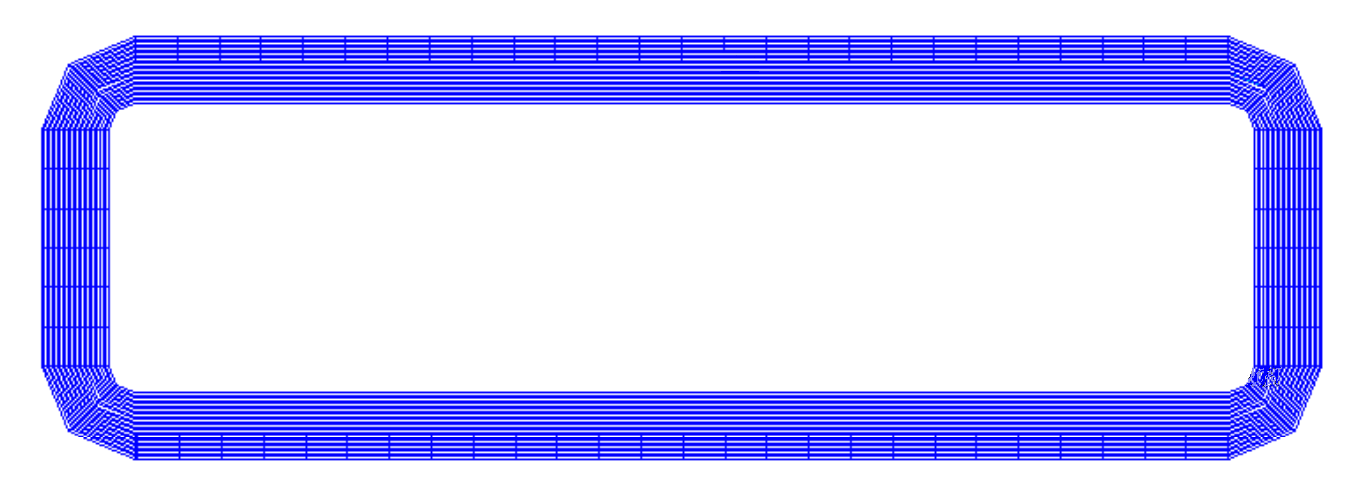
\includegraphics[width=.7\textwidth]{sections/skew_quad_q_det/figures/skew_quad_analysis/coil_top_view.png}};
    \end{tikzpicture}
    \caption{ANSYS meshed geometry of the skew quadrupole - top view.}
    \label{fig:skew_quad_ansys_top_view}
\end{figure}

Parameters of the meshed geometry are summarised in Table~\ref{table: skew_quad_geometry_mesh}. They are based on the discussion in Section~\ref{subsection:update_skew_quadrupole_geometry}. The insulation domain transverse to the strand is equal to $L_\text{ins}=0.07~\text{mm}$ that corresponds to the thickness of a real insulation layer (of only one strand) without resin. The insulation conduction area $A_\text{ins, cond}$ remains unchanged in this set of analyses, i.e. $u_\text{ins}=1.0$. The geometry is discretised on each side of the coil to uniformly distribute the the insulation conduction area $A_\text{ins, cond}$ along the entire domain of the windings. The parameter $n_\text{divisions, insulation}$ corresponds to an average length of a coil rounding. The parameters $n_\text{divisions, side d}$ and $n_\text{divisions, side e}$ refer to Fig.~\ref{fig: winding_length_in_skew_quad}.

There are 72 nodes in each winding representing the composite strand. The insulation layer of every winding is reduced to two elements. It means that the insulation layer between two neighbouring windings accounts for four elements out of which two are coupled with one another. Therefore, the insulation modelling sustains a basic condition of simulating non-linear phenomena that require using at minimum three nodes. The longitudinal mesh size is equal to 15~mm whereas the insulation mesh size -- 35~$\upmu \text{m}$. The entire discretised model accounts for approximately half a million of nodes. Reducing the number of insulation elements aims at lowering the total model size.

\begin{table}[H]
    \caption{Geometry and mesh characteristics.} 
    \vspace{-1.em} 
    \fontsize{10}{10}
    \selectfont 
    \renewcommand{\arraystretch}{1.5}
    \begin{center}
        \begin{tabular}{ ccc }  
        \hline
        parameter & value & unit \\
        \hline
        $L_\text{coil, ANSYS}$ & 809.9 & [m] \\
        $L_\text{ins}$ & 0.07 & [mm] \\
        $A_\text{ins, cond}$ & $8.75 \cdot 10^{-6}$ & [$\text{m}^2$] \\
        $u_\text{ins}$ & 1.0 & [-] \\
        $n_\text{divisions, insulation}$ & 2 & [-] \\
        $n_\text{divisions, winding}$ & 64 & [-] \\
        $n_\text{divisions, side d}$ & 26 & [-] \\
        $n_\text{divisions, side e}$ & 6 & [-] \\
        mesh size, insulation & 35 & [$\upmu \text{m}$] \\
        average mesh size, strand & 15 & [mm] \\ 
        nodes in coil & 478 000 & [-] \\
        \hline 
        \end{tabular}
    \end{center}  
     \label{table: skew_quad_geometry_mesh} 
 \end{table}

There are three quench analyses conducted with a varying heat capacity of resin that refers to the parameter $u_\text{resin}$, as depicted in Table~\ref{table: skew_quad_geometry_cases}. Adding 0D elements to the strand increases the total number of elements in the model from 480 000 to 530 000. 

\begin{table}[H]
    \caption{Geometry and mesh characteristics.} 
    \vspace{-1.em} 
    \fontsize{10}{10}
    \selectfont 
    \renewcommand{\arraystretch}{1.5}
    \begin{center}
        \begin{tabular}{ c | c | c }  
        \hline
        $u_\text{resin}$ & $V_\text{MASS71}$, [$\text{m}^3$] & elements in coil \\
        \hline
        0.0 & 0.0 & 476 528 \\
        0.5 & $2.4 \cdot 10^{-9}$ & 531 574 \\
        1.0 & $4.8 \cdot 10^{-9}$ & 531 574 \\
        \hline 
        \end{tabular}
    \end{center}  
     \label{table: skew_quad_geometry_cases} 
 \end{table}

\subsection{Analysis Settings}

The co-simulation time window remains identical with respect to the previous chapters, as depicted in Table~\ref{table: skew_quad_quench_detect_input_params}. The ANSYS simulation time step is assumed to be constant and equal to the maximum value of a time step range used for the quench velocity-based approach in Chapter~\ref{chapter:quench_velocity_benchmarking}. The time step is increased to keep the computing time in a reasonable limit of several days. The initial energy deposition is placed in the centre of a winding directly neighbouring with the spot heater corresponding to the position of 367.67~m in the meshed model.

\begin{table}[H]
    \caption{Input parameters in the quench detection analysis of the skew quadrupole.} 
    \vspace{-1.em} 
    \fontsize{10}{10}
    \selectfont 
    \renewcommand{\arraystretch}{1.5}
    \begin{center}
        \begin{tabular}{ ccc }  
        \hline
        parameter & value & unit \\
        \hline
        $t_\text{com}$ & 2.5 & [ms] \\
        $t_\text{step}$ & 1 & [ms] \\ 
        hot-spot position in coil & 367.97 & [m] \\
        \hline 
        \end{tabular}
    \end{center}  
     \label{table: skew_quad_quench_detect_input_params} 
 \end{table}

\subsection{Results}

The evolution of resistive voltage until the quench detection is shown in Fig.~\ref{fig: quench_detection_v_res}. The results from three analyses are compared with the measurements. One can observe that the~initial slope of the~simulated models and the measured magnet remains similar at $t < 0.1~\text{s}$. It means that the~initial quench velocity set in the model corresponds to its real value in the quenched winding at $I=86~\text{A}$. In the measurements, the first turn-to-turn propagation occurs at $t \approx 0.08~\text{s}$ which is much faster than in case of each simulation. However, one must remember that the initial heat impulse is much larger in the measurements than in the simulated cases. Therefore, the~first transverse propagation also occurs more slowly in the simulations compared to the measurements. Including resin in the models results in a slower turn-to-turn propagation as well. Such a phenomenon is expected due to a higher heat capacity of the windings with resin. 

\begin{figure}[H]
    \centering
    \begin{tikzpicture}
        \begin{axis}[
          no markers,
          width=0.7\linewidth, 
          height = 4.0cm,
          xlabel={$t,~\text{s}$},
          ylabel={$V_\text{res},~\text{V}$},
          xmin=0.0,
          xmax=0.5,
          xtick= {0,0.1,0.2,0.3,0.4,0.5},
          ymin=0.0,
          ymax=0.5,
          legend pos = outer north east
          ]
          
          \addplot[green] table[x=time,y=V_res,col sep=comma] {sections/skew_quad_q_det/figures/skew_quad_analysis/results_case1.csv}; 
          
          \addplot[blue] table[x=time,y=V_res,col sep=comma] {sections/skew_quad_q_det/figures/skew_quad_analysis/results_case2.csv}; 
          
          \addplot[red] table[x=time,y=V_res,col sep=comma] {sections/skew_quad_q_det/figures/skew_quad_analysis/results_case3.csv}; 
          
          \addplot[black, dashed] table[x=time,y=V_res,col sep=comma] {sections/skew_quad_q_det/figures/skew_quad_analysis/measurements.csv}; 
          
          \addplot[black, dotted] table[x=time,y=QDS_v_threshold,col sep=comma] {sections/skew_quad_q_det/figures/skew_quad_analysis/measurements.csv}; 
          
          \legend{
          $u_\text{resin}=0.0$,
          $u_\text{resin}=0.5$,
          $u_\text{resin}=1.0$,
          measurements}
          
        \end{axis}
    \end{tikzpicture}
    \caption{Rise of resistive voltage.}
    \label{fig: quench_detection_v_res}
\end{figure}

Once the first turn-to-turn propagation occurs, the simulated models start resembling the measurements because the current discharged in the coil becomes a predominant heat source. In order to compare the measurements with the performed analyses, each resistive voltage obtained in the simulations is translated to the left so that the~threshold voltage $V_\text{th}$ is reached at the same time window. Table~\ref{table: skew_quad_v_res_q_det} presents the~time windows at which the~threshold voltage is obtained for every case. The translation times are used in the next section to translate the plots of the resistive  voltage and resistance from the simulations. By that means, the comparison of the simulations with the results is more clear. 

\begin{table}[H]
    \caption{List of time windows at which the simulations reaches $V_\text{th}$.} 
    \vspace{-1.em} 
    \fontsize{10}{10}
    \selectfont 
    \renewcommand{\arraystretch}{1.5}
    \begin{center}
        \begin{tabular}{ cccc }  
        \hline
        parameter & $t(V_\text{th})$ & $t_\text{translation}$ & unit \\
        \hline
        measurements & 0.13 & - & [s] \\
        $u_\text{resin}=0$ & 0.30 & -0.17 & [s] \\
        $u_\text{resin}=0.5$ & 0.36 & -0.23 & [s] \\
        $u_\text{resin}=1.0$ & 0.40 & -0.27 & [s] \\
        \hline 
        \end{tabular}
    \end{center}  
     \label{table: skew_quad_v_res_q_det} 
 \end{table}

\section{Analysis of Magnet Discharge}

\subsection{Additional Input Parameters}

The quench is detected 20~ms after the threshold voltage $V_\text{th}$ is reached (see Table~\ref{table:qds_characteristics}). At that moment, ANSYS solves a discharge of an RL-circuit with an initially applied current of $I=86~\text{A}$. The model takes into account the nonlinear inductance of  the magnet presented in Fig.~\ref{fig:differential_inductance}.

\begin{figure}[H]
    \centering
    \begin{tikzpicture}
        \begin{axis}[
          no markers,
          legend style={at={(1,0)},anchor=south east},
          grid=both, 
          grid style={dashed,gray!30},
          width=0.7\linewidth, 
          height = 5cm,
          xlabel={$I,~\text{A}$},
          ylabel={$L_\text{d},~\text{H}$},
          xlabel style={below right},
          ylabel style={above left},
          xmin=0.0,
          xmax=100.0,
          ymin=0.0,
          ymax=6.0
          ]
          \addplot table[x=current,y=inductance,col sep=comma] {sections/skew_quad_q_det/figures/skew_quad_analysis/differential_inductance.csv}; 
        \end{axis}
    \end{tikzpicture}
    \caption{Differential inductance as a function of current for the skew quadrupole~\cite{marco_prioli_mails}.}
    \label{fig:differential_inductance}
\end{figure}

The circuit represented in Fig.~\ref{fig:skew_quad_discharge_electrical_scheme} is solved with additional electrical elements in ANSYS -- CIRCU124. Resistors and inductors modelled by CIRCU124 elements have voltage as a~single degree of freedom~\cite{ansys_element_manual}. The non-linear inductor is modelled by updating its inductance at each communication point between Python and ANSYS. Table~\ref{table: skew_quad_discharge_input_params} depicts additional simulation parameters for the discharge phase of the magnet. 

\begin{table}[H]
    \caption{Input parameters in the analysis of the skew quadrupole discharge.} 
    \vspace{-1.em} 
    \fontsize{10}{10}
    \selectfont 
    \renewcommand{\arraystretch}{1.5}
    \begin{center}
        \begin{tabular}{ ccc }  
        \hline
        parameter & value & unit \\
        \hline
        communication time step before the entire coil quenches & 0.0025 & [s] \\
        communication time step after the entire coil quenches & 0.2 & [s] \\ 
        material properties update criterion & 10 & [A] \\ 
        magnet discharge criterion & 8 & [A] \\
        \hline 
        \end{tabular}
    \end{center}  
     \label{table: skew_quad_discharge_input_params} 
 \end{table}

The quench velocity-based approach is only needed until the entire coil quenches. Therefore, after that moment, the communication time step is increased to $t=0.2~\text{s}$. The remaining communication time steps are required for updating the inductance of a magnet and extracting the value of current. Updating varying material properties, being a function of magnetic field, for 754 windings is a time-consuming process. Thus, it is only conducted if the current in the magnet drops by $I=10~\text{A}$ meaning that the magnetic field also decreases. It is assumed that the magnet is fully discharged if the transport current drops below $I=8~\text{A}$, i.e. if the current decreased by 90\% of its initial value.

\subsection{Results}

Fig.~\ref{fig: magnet_discharge_v_res} presents the evolution of resistive voltage $V_\text{res}$ in time. The higher volume ratio is considered in the model, the lower peak resistive voltage is obtained. Moreover, the peak voltage occurs faster with lower $c_\text{volume}$. In principle, the~peak voltage corresponds to a~moment when both longitudinal and turn-to-turn quench propagation result in a quench of the entire coil. In Fig.~\ref{fig: magnet_discharge_v_res}, one can also notice sharp changes of resistive voltage which occur in gradually increasing time periods. These changes are due to an update of material properties at each $I=10~\text{A}$.

\begin{figure}[H]
    \centering
    \begin{tikzpicture}
        \begin{axis}[
          no markers,
          width=0.8\linewidth, 
          height = 6.5cm,
          xlabel={$\text{Time},~\text{s}$},
          ylabel={$V_\text{res},~\text{V}$},
          xmin=0.0,
          ymin=0.0,
          ymax=30.0,
          legend pos = north east
          ]
          
          \addplot[green] table[x=time_delayed,y=V_res,col sep=comma] {sections/skew_quad_q_det/figures/skew_quad_analysis/results_case1.csv}; 
          
          \addplot[blue] table[x=time_delayed,y=V_res,col sep=comma] {sections/skew_quad_q_det/figures/skew_quad_analysis/results_case2.csv}; 
          
          \addplot[red] table[x=time_delayed,y=V_res,col sep=comma] {sections/skew_quad_q_det/figures/skew_quad_analysis/results_case3.csv}; 
          
          \addplot[black, dashed] table[x=time,y=V_res,col sep=comma] {sections/skew_quad_q_det/figures/skew_quad_analysis/measurements.csv}; 
          
          \legend{
          $c_\text{volume}=0.0$,
          $c_\text{volume}=0.5$,
          $c_\text{volume}=1.0$,
          measurements}
          
        \end{axis}
    \end{tikzpicture}
    \caption{Coil resistive voltage change in time.}
    \label{fig: magnet_discharge_v_res}
\end{figure}

Every simulation results in an overestimation of the peak resistive voltage with respect to the measurements. It is directly connected to the change of coil resistance during the~discharge presented in Fig.~\ref{fig: magnet_discharge_resistance}. The higher resin volume is included in the model, the~lower coil resistance is obtained. It is an expected result because resin is an additional thermal capacitance meaning that the coil remains at a lower temperature. 

\begin{figure}[H]
    \centering
    \begin{tikzpicture}
        \begin{axis}[
          no markers,
          width=0.8\linewidth, 
          height = 6.5cm,
          xlabel={$\text{Time},~\text{s}$},
          ylabel={$R_\text{coil},~\Upomega$},
          xmin=0.0,
          ymin=0.0,
          ymax=1.0,
          legend pos = south east
          ]

          \addplot[green] table[x=time_delayed,y=Resistance,col sep=comma] {sections/skew_quad_q_det/figures/skew_quad_analysis/results_case1.csv}; 
          
          \addplot[blue] table[x=time_delayed,y=Resistance,col sep=comma] {sections/skew_quad_q_det/figures/skew_quad_analysis/results_case2.csv}; 
          
          \addplot[red] table[x=time_delayed,y=Resistance,col sep=comma] {sections/skew_quad_q_det/figures/skew_quad_analysis/results_case3.csv}; 
          
          \addplot[black, dashed] table[x=time,y=Resistance,col sep=comma] {sections/skew_quad_q_det/figures/skew_quad_analysis/measurements.csv}; 
          
          \legend{
          $c_\text{volume}=0.0$,
          $c_\text{volume}=0.5$,
          $c_\text{volume}=1.0$,
          measurements}
          
        \end{axis}
    \end{tikzpicture}
    \caption{Coil resistance evolution in time.}
    \label{fig: magnet_discharge_resistance}
\end{figure}

The final temperature of the coil for every simulated case is shown in Fig.~\ref{fig: magnet_discharge_final_temperature}. The~temperature profile inside of a coil can be compared to a sinusoidal signal with a maximum amplitude of approximately $T=15~\text{K}$. The initially quenched winding is the only place with a distinct temperature difference. The initially quenched zone remained the place in the coil characterised by the highest temperature.

\begin{figure}[H]
    \centering
    \begin{tikzpicture}
        \begin{axis}[
          no markers,
          width=0.8\linewidth, 
          height = 7.0cm,
          xlabel={$L_\text{coil},~\text{m}$},
          ylabel={$T,~\text{K}$},
          xmin=0.0,
          xmax=812.0,
          ymin=0.0,
          ymax=50.0,
          legend pos = south east
          ]

          \addplot[green] table[x=METERS,y=case1,col sep=comma] {sections/skew_quad_q_det/figures/skew_quad_analysis/final_magnet_temperature.csv}; 
          
          \addplot[blue] table[x=METERS,y=case2,col sep=comma] {sections/skew_quad_q_det/figures/skew_quad_analysis/final_magnet_temperature.csv}; 
          
          \addplot[black, dashed] table[x=METERS,y=T_init,col sep=comma] {sections/skew_quad_q_det/figures/skew_quad_analysis/final_magnet_temperature.csv}; 
          
        %   \addplot[red] table[x=time,y=Hot_spot,col sep=comma] {sections/skew_quad_q_det/figures/skew_quad_analysis/results_case3.csv}; 
          
          \legend{
          $c_\text{volume}=0.0$,
          $c_\text{volume}=0.5$,
          $T_\text{init}$
        %   $c_\text{volume}=1.0$
          }
          
        \end{axis}
    \end{tikzpicture}
    \caption{Final temperature of the coil after the discharge.}
    \label{fig: magnet_discharge_final_temperature}
\end{figure}

The evolution of the hot spot temperature temperature in time is presented in Fig.~\ref{fig: magnet_discharge_hot_spot}. It can be concluded that the higher resin volume is taken into consideration, the lower hot spot temperature is obtained in the model. 

\begin{figure}[H]
    \centering
    \begin{tikzpicture}
        \begin{axis}[
          no markers,
          width=0.8\linewidth, 
          height = 5.0cm,
          xlabel={$\text{Time},~\text{s}$},
          ylabel={$T_\text{hot spot},~\text{K}$},
          xmin=0.0,
          ymin=0.0,
          ymax=60.0,
          legend pos = south east
          ]

          \addplot[green] table[x=time,y=Hot_spot,col sep=comma] {sections/skew_quad_q_det/figures/skew_quad_analysis/results_case1.csv}; 
          
          \addplot[blue] table[x=time,y=Hot_spot,col sep=comma] {sections/skew_quad_q_det/figures/skew_quad_analysis/results_case2.csv}; 
          
        %   \addplot[red] table[x=time,y=Hot_spot,col sep=comma] {sections/skew_quad_q_det/figures/skew_quad_analysis/results_case3.csv}; 
          
          \legend{
          $c_\text{volume}=0.0$,
          $c_\text{volume}=0.5$,
        %   $c_\text{volume}=1.0$
          }
          
        \end{axis}
    \end{tikzpicture}
    \caption{Hot spot temperature evolution in time.}
    \label{fig: magnet_discharge_hot_spot}
\end{figure}

The current discharge curves are presented in Fig.~\ref{fig: magnet_discharge_current}. The discharge occurs faster in all simulated cases with respect to the measurements. It is a result of a higher coil resistance compared to the measurements. Thus, the time constant (actually varying) in (\ref{eqn:variable_time_constant}) is higher and the current drop is quicker. 

There is one additional analysis added to the plot in which the coil resistance is omitted. The communication time step, at which the inductance is updated, equals $t=0.0025~\text{s}$. The~ANSYS time step in this case is also lower and equal to $t=0.1~\text{ms}$. The higher precision is due to the fact that such a simulation (with already more accurate input parameters) is much faster with respect to the analysis of an entire coil domain. This analysis with no coil resistance represents a case when the magnet discharge is only dependent on the dump resistor of the energy extraction system.

\begin{figure}[H]
    \centering
    \begin{tikzpicture}
        \begin{axis}[
          no markers,
          width=0.8\linewidth, 
          height = 7.5cm,
          xlabel={$\text{Time},~\text{s}$},
          ylabel={$I,~\text{A}$},
          xmin=0.0,
          ymin=0.0,
          legend pos = north east
          ]

          \addplot[green] table[x=time_delayed,y=Current,col sep=comma] {sections/skew_quad_q_det/figures/skew_quad_analysis/results_case1.csv}; 
          
          \addplot[blue] table[x=time_delayed,y=Current,col sep=comma] {sections/skew_quad_q_det/figures/skew_quad_analysis/results_case2.csv}; 
          
          \addplot[red] table[x=time_delayed,y=Current,col sep=comma] {sections/skew_quad_q_det/figures/skew_quad_analysis/results_case3.csv}; 
          
          \addplot[black] table[x=t_translated,y=I_coil,col sep=comma] {sections/skew_quad_q_det/figures/skew_quad_analysis/results_case0.csv};
                    
          \addplot[black, dashed] table[x=time,y=Current,col sep=comma] {sections/skew_quad_q_det/figures/skew_quad_analysis/measurements.csv}; 

          \legend{
          $c_\text{volume}=0.0$,
          $c_\text{volume}=0.5$,
          $c_\text{volume}=1.0$,
          $R_\text{coil} = 0.0$,
          measurements}
          
        \end{axis}
    \end{tikzpicture}
    \caption{Current discharge curve of the skew quadrupole.}
    \label{fig: magnet_discharge_current}
\end{figure}





\section{General Remarks}

Three simulated cases of the magnet discharge allowed for predicting the final temperature profile of the coil, including the evolution of the hot-spot temperature. In principle, when a turn-to-turn propagation is considered, the temperature rise in the hot-spot is less steep than in case of a 1D longitudinal heat propagation, because a part of the accumulated heat is evacuated to neighbouring windings. Therefore, the multi-strand analysis allows for lowering the safety coefficients with respect to the peak hot-spot temperature in case of a quench. On the other hand, the skew quadrupole model overestimates the temperature distribution in the coil regardless of the analysis case conducted with or without resin. Such a conclusion can be made by observing the curves of coil resistance being higher than in case of the measurements. An overestimation of the temperature in the coil is contradictory to the assumptions related to the quench velocity-based approach in which the temperature is underestimated as outlined in Chapter~\ref{chapter:quench_velocity_benchmarking}. The discrepancy in the results with respect to the measurements can be explained as follows: 

\begin{enumerate}
    \item The mesh size across the insulation is relatively large when the entire skew quadrupole is simulated. As discussed in Section~\ref{section:quench_velocity_benchmarking_with_insulation_heat_balance}, a coarser mesh across the insulation results in an overestimation of the hot-spot temperature (see Fig.~\ref{fig: q_vel_modelling_v_quench_hot_spot_temp_with_insulation}).
    \item No influence of helium is considered. In principle, helium is an important additional heat capacity in the system that should reduce the coil temperature during the discharge.
    \item The insulation and resin are homogenised and modelled with G10. The material properties of G10 are assumed to be similar to S2-glass and CTD-101K epoxy resin. By comparing the simulation results with and without resin, it can be concluded that the heat capacity of the coil elements not belonging to the composite strand have a considerable influence on the temperature evolution of the system during the discharge.
\end{enumerate}

By taking the aforementioned arguments into account, it can be concluded, that the model is validated against available measurements of the magnet discharge while assuming a given accuracy. The overestimation of the quench velocity-based approach for the skew quadrupole remains in the range of 50-120\% with respect to the peak resistive voltage. In fact, an overestimation of the resistive voltage or the hot-spot temperature increases the safety margin from the magnet design standpoint. Therefore, it is a favourable case of the discrepancy between the model and the measurements. 

\clearpage
\chapter{Summary}
\label{chapter:research_questions_discussions}

First of all, the physics implemented in ANSYS models was cross-checked in this thesis with STEAM-BBQ, being a standard tool at TE-MPE-PE Section to simulate a 1D quench propagation. Then, the quench velocity-based approach was introduced, which aims at reducing the number of degrees of freedom in the quench problem allowing for simulating a full-scale coil of a magnet. The ANSYS models and the algorithms governing the quench velocity-based approach were described. The quench velocity-based approach was verified with standard ANSYS simulations, which do not apply the proposed method (instead, they are based on the heat balance equation). The aim of this study was to estimate the error associated with relaxing the mesh density in the quench velocity-based approach. The verification between the standard ANSYS analysis and the quench velocity-based approach was conducted with simplified models only simulating the longitudinal quench propagation. The quench velocity-approach allowed for simulating the skew quadrupole discharge being one of the high-order corrector magnets for the HL-LHC upgrade. One coil of the magnet was simulated in which both the longitudinal and the turn-to-turn propagation were analysed and validated against available measurements.

The implementation of the quench velocity-based approach leads to a considerable decrease in the number of degrees of freedom of the numerical model. The lower number of degrees of freedom allows for simulating a full-scale coil of a magnet. Nevertheless, the simulation remains an approximation, in which a certain error should be considered. It is recommended to take the error into account because the key magnet design parameters, such as the hot-spot temperature as well as the voltage-to-ground, are underestimated in the quench velocity-based approach with respect to a standard numerical solution. In the quench velocity-based approach, the improvement rate in computation time is the highest when an external insulation layer (optionally including the epoxy resin) with a relatively high number of nodes is simulated. In this case, a high mesh relaxation in the longitudinal direction of the coil allows for a considerable decrease in the number of insulation nodes nodes with respect to the standard numerical analysis. Based on the example of the skew quadrupole, the discharge of the magnet, in which the quench occurs in one coil, can be simulated within five-seven days. Unfortunately, even the quench velocity-based approach did not allow for simulating the skew quadrupole with a refined insulation layer due to an exceeding computation time. The mesh refinement of 20 elements across the insulation would make the model too heavy to compute for ANSYS (in the order of 4 million elements). Therefore, the high improvement of the computation time is not visible when the quench velocity-based approach is used. In principle, the more accurate a discretisation of the insulation layer is applied in the model, the higher the gain in the computation time that is reached with the quench velocity-based approach as compared to a standard analysis with the same mesh across the insulation. Overall, the multi-strand quench simulation of full coils, relying on the quench velocity-based approach, will remain a tool implemented in the final design stage of the quench protection study, rather than in its beginning when short iteration loops are required.

The quench velocity-based approach is successfully implemented in ANSYS by using an external routine developed in Python imposing the position of the quenched zone as the simulation proceeds. The ANSYS model allows for studying the current discharge in an RL-circuit with a constant dump resistance and the inductance being a function of the transport current. It is possible to neglect the dump resistance in case of future quench simulations of self-protected magnets. The temperature evolution inside of the coil relies on the longitudinal and the turn-to-turn quench propagation. Moreover, the material properties are a function of temperature and magnetic field strength during the quench propagation in a magnet. The~simulation of the full magnet discharge requires using the following ANSYS elements: 

\begin{enumerate}
    \item LINK68 used for the composite strand.
    \item LINK33 applied to simulate the insulation layer.
    \item CIRCU124 required for connecting the coil to an external power source (independent current source), resistor and inductor.
    \item MASS71 optionally used to take resin into account when fully impregnated coils are simulated. Moreover, a part of the insulation layer may also be compressed in the given elements.
\end{enumerate}


% APPENDICES
\clearpage
\begin{appendices}

\chapter{Material Properties}
\label{appendix_material_properties_description}

The material properties used in this thesis are presented and discussed in the following Appendix. Since July 2019, it is recommended at TE-MPE-PE to use material fit functions provided by NIST. Except for the volumetric heat capacity of Nb-Ti, which NIST does not provide, all material properties are based on an update ROXIE\footnote{ROXIE is CERN internal software for electromagnetic simulation and optimisation of accelerator magnets.} database prepared at CERN \cite{material_properties_roxie}. Nb-Ti is defined based on CUDI being Arjan Verweij's CERN internal routine for modelling of superconducting strands and cables~\cite{cudi_manual}.

\section{Copper}
\label{appendix:cu_material_properties}

\subsection{RRR}
\label{appendix:subsection_rrr_definition}
Residual resistivity ratio, RRR is a parameter comparing copper resistivity at two different temperatures when no magnetic field is applied. It is calculated as: 
\begin{equation}
\text{RRR} = \frac{\rho(T_\text{high}, B=0~\text{T})}{\rho(T_\text{low}, B=0~\text{T})},
\end{equation}
where $T_\text{high}=273~\text{K}$ and $T_\text{low}=4~\text{K}$.

\subsection{Resistivity}
Copper resistivity depends on temperature and RRR:
\begin{equation}
    \rho_\text{N}(T, \text{RRR}) = \rho_\text{0}+\rho_\text{i}+\rho_\text{i0},
\end{equation}
\\
where:
\begin{equation}
    \rho_\text{0} = \frac{1.5553\cdot10^{-8}}{\text{RRR}},
\end{equation}

\begin{equation}
    \rho_\text{i} = \frac{\text{P}_\text{1}}{1+\text{P}_\text{1}  \text{P}_\text{3}, T^{\text{P}_\text{2} - \text{P}_\text{4}}, \exp{[-(\frac{\text{P}_\text{5}}{T}}^{\text{P}_\text{6}})]},
\end{equation}

\begin{equation}
    \rho_\text{i0} = \text{P}_\text{7} \frac{\rho_\text{i} \rho_\text{0}}{\rho_\text{i} + \rho_\text{0}},
\end{equation}
with fit parameters depicted in Table \ref{table:nist_resistivity_parameters}. 

\begin{table}[H]
    \caption{Fit P-parameters for copper electrical resistivity} 
    \vspace{-1.em} 
    \fontsize{10}{10}
    \selectfont 
    \renewcommand{\arraystretch}{1.5}
    \begin{center}
    \begin{tabular}{ ccccccc }  
    \hline
    $\text{P}_1$ & $\text{P}_2$ & $\text{P}_3$ & $\text{P}_4$ & $\text{P}_5$ & $\text{P}_6$ & $\text{P}_7$ \\
    \hline
    $1.171\cdot10^{-17}$ & 4.49 & $3.841\cdot10^{10}$ & 1.14 & 50 & 6.428 & 0.4531 \\
    \hline 
    \end{tabular}
    \end{center}  
     \label{table:nist_resistivity_parameters} 
 \end{table}
 
In order to apply the resistivity dependence on magnetic field strength, the following formula is applied:

\begin{equation}
    \rho_\text{N}(T, B, \text{RRR}) = \rho_\text{N}(T, \text{RRR}) \cdot (1 + 10^{a(x)}),  
\end{equation}
where:
\begin{equation}
    a(x) = \sum_{n=0}^{N} a_\text{n}(\log_\text{10}x)^{n},
\end{equation}

\begin{equation}
    x \approx \frac{1.553 \cdot 10^{-8}}{\rho_\text{N}(T, \text{RRR})} \cdot B,
\end{equation}
with $B$ -- magnetic field strength, $a$ -- fit parameters described in Table \ref{table:nist_resistivity_parameters2}.

\begin{table}[h!]
    \caption{Fit a-parameters for copper electrical resistivity} 
    \vspace{-1.em} 
    \fontsize{10}{10}
    \selectfont 
    \renewcommand{\arraystretch}{1.5}
    \begin{center}
    \begin{tabular}{ ccccc }  
    $\text{a}_0$ & $\text{a}_1$ & $\text{a}_2$ & $\text{a}_3$ & $\text{a}_4$ \\
    \hline
    -2.662 & 0.3168 & 0.6229 & -0.1839 & 0.001827 \\
    \hline
    \end{tabular}
    \end{center}  
     \label{table:nist_resistivity_parameters2} 
 \end{table}

As presented in Fig. \ref{fig:cu_resistivity_plot}, the resistivity of copper rises with rise of temperature. It rises with increase of magnetic field strength as well as with decrease of RRR.

\begin{figure}[H]
\centering
\begin{tikzpicture}
\begin{axis}[
  no markers,
  legend style={at={(1,0)},anchor=south east},
  grid style={dashed,gray!30},
  width=0.85\linewidth, 
  height = 6cm,
  xlabel={$T,~\text{K}$},
  ylabel={$\rho,~\Omega~\text{m}$},
  xlabel style={below right},
  ylabel style={above left},
  xmin=0.0,
  ymin=0.0,
  xmax=100.0,
  legend pos=north west
  ]
  \addplot table[x=Time,y=B_0_0_RRR_200,col sep=comma] {sections/appendices/material_properties/copper/figures/cu_resistivity.csv}; 
  \addplot table[x=Time,y=B_3_0_RRR_200,col sep=comma] {sections/appendices/material_properties/copper/figures/cu_resistivity.csv}; 
  
  \legend{
  \textit{B}(RRR=200)=0 T,
  \textit{B}(RRR=200)=3 T}

\end{axis}
\end{tikzpicture}
\caption{Copper resistivity temperature dependence for two values of magnetic field.}
    \label{fig:cu_resistivity_plot}
\end{figure}

%  thermal conductivity
\subsection{Thermal Conductivity}
\label{subsection:copper_thermal_conductivity}
Copper thermal conductivity depends on temperature and RRR:
\begin{equation}
    k_\text{N}(T, \text{RRR}) = \frac{1}{\text{W}_\text{0} + \text{W}_\text{i} + \text{W}_\text{i0}}, 
\end{equation}
where:
\begin{equation}
    \text{W}_\text{0} = \frac{\beta}{T},
\end{equation}

\begin{equation}
    \text{W}_\text{i} = \frac{\text{P}_\text{1} T^{\text{P}_\text{2}}}{1+\text{P}_\text{1}  \text{P}_\text{3}  T^{\text{P}_\text{2} + \text{P}_\text{4}}  \exp{[-(\frac{\text{P}_\text{5}}{T}}^{\text{P}_\text{6}})]},
\end{equation}

\begin{equation}
    \text{W}_\text{i0} = \text{P}_\text{7} \frac{\text{W}_\text{i} \text{W}_\text{0}}{\text{W}_\text{i} + \text{W}_\text{0}},
\end{equation}
\\
with fit parameters presented in Table \ref{table:nist_cu_k_parameters}.

\begin{table}[H]
    \caption{Fit \textbeta- and P-parameters for copper thermal conductivity} 
    \vspace{-1.em} 
    \fontsize{10}{10}
    \selectfont 
    \renewcommand{\arraystretch}{1.5}
    \begin{center}
    \begin{tabular}{ cc }  
    $\upbeta$ & $\upbeta_\text{r}$ \\
    \hline
    $0.634/\text{RRR}$ & $\upbeta/0.0003$ \\
    \hline
    \end{tabular}
    
    \begin{tabular}{ ccccccc }  
    $\text{P}_1$ & $\text{P}_2$ & $\text{P}_3$ & $\text{P}_4$ & $\text{P}_5$ & $\text{P}_6$ & $\text{P}_7$ \\
    \hline
    $1.754\cdot10^{-8}$ & 2.763 & 1102 & -0.165 & 70 & 1.756 & $0.838/\upbeta_\text{r}^{0.1661}$ \\
    \hline 
    \end{tabular}
    \end{center}  
     \label{table:nist_cu_k_parameters} 
 \end{table}
 
 In order to include the magnetic induction dependence in the function of thermal conductivity, the following formula is applied: 
\begin{equation}
    k_\text{N}(T, B, \text{RRR}) = \frac{\rho\text{N}(T, B=0, \text{RRR})}{\rho\text{N}(T, B=0, \text{RRR})} \cdot k_\text{N}(T, \text{RRR})
\end{equation}

As presented in Fig. \ref{fig:cu_k_plot}, the thermal conductivity of copper decreases with rise of magnetic field strength. One can also notice that the peak value of thermal conductivity is higher with increase of RRR. 
 
\begin{figure}[H]
\centering
\begin{tikzpicture}
\begin{axis}[
  no markers,
  legend style={at={(1,0)},anchor=south east},
  grid style={dashed,gray!30},
  width=0.85\linewidth, 
  height = 6cm,
  xmode=log,
  xlabel={$T,~\text{K}$},
  ylabel={$k,~\frac{\text{W}}{\text{m K}}$},
  xlabel style={below right},
  ylabel style={above left},
  xmax=300.0,
  ymin=0.0,
  ymax=4200.0,
  legend pos=north west
  ]
  \addplot[smooth, blue] table[x=temperature,y=B0,col sep=comma] {sections/appendices/material_properties/copper/figures/cu_thermal_conductivity_rrr_200.csv}; 
  \addplot[smooth, red] table[x=temperature,y=B3,col sep=comma] {sections/appendices/material_properties/copper/figures/cu_thermal_conductivity_rrr_200.csv};

  \addplot[smooth, dashed, blue] table[x=temperature,y=B0,col sep=comma] {sections/appendices/material_properties/copper/figures/cu_thermal_conductivity_rrr_50.csv};
  \addplot[smooth, dashed, red] table[x=temperature,y=B3,col sep=comma] {sections/appendices/material_properties/copper/figures/cu_thermal_conductivity_rrr_50.csv};

  \legend{
  \textit{B}(RRR=200)=0 T,
  \textit{B}(RRR=200)=3 T,
  \textit{B}(RRR=50)=0 T,
  \textit{B}(RRR=50)=3 T}

\end{axis}
\end{tikzpicture}
\caption{Thermal conductivity of copper as a function of temperature for two values of magnetic field and RRR.}
    \label{fig:cu_k_plot}
\end{figure}

% mass density 
\subsection{Mass Density}
The mass density of copper is assumed to be constant and equal to $\rho = 8960~\text{kg/m}^{3}$.

% Volumetric heat capacity 
\subsection{Volumetric Heat Capacity}
Copper specific heat capacity is approximated with a polynomial interpolation as: 
\begin{equation}
    x(T) = 10^{\sum_{n=0}^{N} a_\text{n}(\log_\text{10}T)^{n}},
\end{equation}
\\
where $N$ -- order of polynomial, a -- fit parameters described in Table \ref{table:nist_cu_cp_parameters}. 

\begin{table}[H]
    \caption{Fit parameters for copper specific heat capacity} 
    \vspace{-1.em} 
    \fontsize{10}{10}
    \selectfont 
    \renewcommand{\arraystretch}{1.5}
    \begin{center}
    \begin{tabular}{ cccccccc }  
    $\text{a}_0$ & $\text{a}_1$ & $\text{a}_2$ & $\text{a}_3$ & $\text{a}_4$ & $\text{a}_5$ & $\text{a}_6$ & $\text{a}_7$ \\
    \hline
    -1.91844 & -0.15973 & 8.61013 & -18.996 & 21.9661 & -12.7328 & 3.54322 & -0.3797 \\
    \hline 
    \end{tabular}
    \end{center}  
     \label{table:nist_cu_cp_parameters} 
 \end{table}
 
In order to convert specific into volumetric heat capacity, the polynomial function is divided by copper density. The volumetric heat capacity of copper is presented in Fig. \ref{fig:cu_cv_plot}.

\begin{figure}[H]
\centering
\begin{tikzpicture}
\begin{axis}[
  no markers,
  legend style={at={(1,0)},anchor=south east},
  grid style={dashed,gray!30},
  width=0.85\linewidth, 
  height = 6cm,
  xlabel={$T,~\text{K}$},
  ylabel={$c_\text{v},~\frac{\text{J}}{\text{m}^3~\text{K}}$},
  xlabel style={below right},
  ylabel style={above left},
  xmin=0.0,
  ymin=0.0,
  xmax=300.0,
  legend pos=north west
  ]
  \addplot[smooth, blue] table[x=temperature,y=cvcu,col sep=comma] {sections/appendices/material_properties/copper/figures/cu_cv.csv}; 

\end{axis}
\end{tikzpicture}
    \caption{Volumetric heat capacity of copper as a function of temperature.}
    \label{fig:cu_cv_plot}
\end{figure}

\section{Niobium Titanium}
\label{appendix:nbti_material_properties}

% NbTi mass density 
\subsubsection{Mass Density}
The mass density is assumed to be constant and equal to $\rho = 6000~\text{kg/m}^{3}$.

% NbTi specific heat capacity
\subsubsection{Specific Heat Capacity}
Volumetric heat capacity of Nb-Ti is estimated by means of a piece-wise polynomial function which takes into account a linear magnetic dependence below the critical temperature. The critical temperature is calculated as: 
\begin{equation}
    T_\text{c}(B) = T_\text{c0}\cdot(1-\frac{B}{B_\text{c20}})^{0.59},
\end{equation}
where $T_\text{c0}$ -- critical temperature for $B=0~\text{T}$, $B_\text{c20}$ -- critical magnetic field for $T=0~\text{K}$. In both parameters, current density is equal to zero.

The volumetric heat capacity is calculated in the following manner: 
\begin{equation}
    Cp_\text{ NbTi}(T, T_\text{c}) = \frac{\text{a}_0 + \text{a}_1\cdot T^{1} + \text{a}_2\cdot T^{2} + \text{a}_3\cdot T^{3}+ \text{a}_4\cdot T^{4}} {\rho_{Nb-Ti}},
\end{equation}
where $a$ -- fit parameters presented in Table \ref{table:nbti_parameters}.

\begin{table}[h!]
    \caption{Polynomial parameters for Nb-Ti volumetric heat capacity.} 
    \vspace{-1.em} 
    \fontsize{10}{10}
    \selectfont 
    \renewcommand{\arraystretch}{1.5}
    \begin{center}
    \begin{tabular}{ lccccc }  
    \hline
    & $\text{a}_0$ & $\text{a}_1$ & $\text{a}_2$ & $\text{a}_3$ & $\text{a}_4$ \\
    \hline
    $T \in (0, T_\text{c})$~K & 0 & $64 \cdot B$ & 0 & 49.1 & 0 \\        
    $T \in [T_\text{c}, 28.358)$~K & 0 & 928 & 0 & 16.24 & 0 \\        
    $T \in [28.358, 50.99)$~K & 41383 & -7846.1 & 553.71 & 11.9838 & -0.2177 \\        
    $T \in [50.99, 165.8)$~K & $-1.53\cdot10^{6}$ & 83022 & -716.3 & 2.976 & -0.00482 \\ 
    $T \in [165.8, 496.54)$~K & $1.24\cdot10^{6}$ & 13706 & -51.66 & 0.09296 & $-6.29\cdot10^{-5}$ \\        
    $T \in [496.54, 1000)$~K & $2.45\cdot10^{6}$ & 955.5 & -0.257 & 0 & 0 \\       
    \hline
     \end{tabular} 
    \end{center}  
     \label{table:nbti_parameters} 
\end{table}

As presented in Fig. \ref{fig:nbti_cv_plot}, there occurs a step jump in Nb-Ti heat capacity at critical temperature. Since the critical temperature decreases with rise of magnetic field strength, the transition occurs at lower temperatures when higher B-field is applied.
 
\begin{figure}[h!]
    \centering
    \begin{tikzpicture}[spy using outlines=
	{circle, magnification=8, connect spies}]
    \begin{axis}[
      no markers,
      legend style={at={(1,0)},anchor=south east},
      grid style={dashed,gray!30},
      width=0.85\linewidth, 
      height = 6cm,
      xlabel={$T,~\text{K}$},
      ylabel={$C_\text{v},~\frac{\text{J}}{\text{m}^3~\text{K}}$},
      xtick={8.5, 50, 100, 150, 200, 250, 300},
      xlabel style={below right},
      ylabel style={above left},
      xmin=0.0,
      ymin=0.0,
      xmax=300.0,
      legend pos=north west
      ]
      \addplot[smooth, blue] table[x=temperature,y=B0,col sep=comma] {sections/appendices/material_properties/niobium_titanium/figures/nb_ti_cv.csv}; 
      \addplot[smooth, red] table[x=temperature,y=B3,col sep=comma] {sections/appendices/material_properties/niobium_titanium/figures/nb_ti_cv.csv}; 
      
      \coordinate (spypoint) at (8.5,20000);
      \coordinate (magnifyglass) at (100, 1000000);
    
      \legend{
      \textit{B}=0 T,
      \textit{B}=3 T}
    
    \end{axis}
    \spy [black, size=2.5cm] on (spypoint)
       in node[fill=white] at (magnifyglass);
    \end{tikzpicture}
    \caption{Volumetric heat capacity of Niobium-Titanium as a function of temperature.}
    \label{fig:nbti_cv_plot}
\end{figure}

\section{G10 Material Properties}
\label{appendix:g10_material_properties}

% thermal conductivity
\subsubsection{Thermal Conductivity}
G10 is an epoxy-impregnated fiberglass, thermally anisotropic. It means that its thermal conductivity along the fibers is higher than across them. In order to simplify computation in the scope of this thesis, the material is assumed to be isotropic. A conservative assumption is made which states that thermal conductivity of G10 in all directions is equal to the one which is normal to the direction of the fibers.
G10 thermal conductivity as well as its specific heat capacity is approximated with the NIST polynomial interpolation as: 
\begin{equation}
    x(T) = 10^{\sum_{n=0}^{N} a_\text{n}(\log_\text{10}T)^{n}},
    \label{G10_polynomial_interpolation}
\end{equation}
\\
where $x(T)$ -- considered material property, $N$ -- order of polynomial, $a$ -- fit parameters described in Table \ref{table:nist_g10_k_parameters}.

\begin{table}[h!]
    \caption{Fit parameters for G10 thermal conductivity} 
    \vspace{-1.em} 
    \fontsize{10}{10}
    \selectfont 
    \renewcommand{\arraystretch}{1.5}
    \begin{center}
    \begin{tabular}{ ccccccccc }  
    $\text{a}_0$ & $\text{a}_1$ & $\text{a}_2$ & $\text{a}_3$ & $\text{a}_4$ & $\text{a}_5$ & $\text{a}_6$ & $\text{a}_7$ & $\text{a}_8$ \\
    \hline
    -4.1236 & 13.788 & -26.068 & 26.272 & -14.663 & 4.4954 & -0.6905 & 0.0397 & 0 \\
    \hline 
    \end{tabular}
    \end{center}  
     \label{table:nist_g10_k_parameters} 
 \end{table}

The thermal conductivity of G10 as a function of temperature is presented in Fig. \ref{fig:g10_k_plot}.

\begin{figure}[h!]
    \centering
    \begin{tikzpicture}
    \begin{axis}[
      no markers,
      legend style={at={(1,0)},anchor=south east},
      grid style={dashed,gray!30},
      width=0.85\linewidth, 
      height = 6cm,
      xlabel={$T,~\text{K}$},
      ylabel={$k,~\frac{\text{W}}{\text{m K}}$},
      xlabel style={below right},
      ylabel style={above left},
      xmin=0.0,
      ymin=0.0,
      xmax=300.0
      ]
      \addplot[smooth, blue] table[x=temperature,y=g10_thermal_conductivity,col sep=comma] {sections/appendices/material_properties/g10/figures/g10_thermal_conductivity.csv}; 
    
    \end{axis}
    \end{tikzpicture}
    \caption{G10 thermal conductivity as a function of temperature.}
    \label{fig:g10_k_plot}
\end{figure}
 
% mass density
 \subsubsection{Mass Density}
 The mass density is assumed to be constant and equal to $\rho = 1948~\text{kg/m}^{3}$.

% specific heat capacity
\newpage
\subsubsection{Volumetric Heat Capacity}
Specific heat capacity of G10 is based on equation described in (\ref{G10_polynomial_interpolation}) with fit parameters described in \ref{table:nist_g10_cp_parameters}. 

\begin{table}[h!]
    \caption{Fit parameters for G10 specific heat capacity} 
    \vspace{-1.em} 
    \fontsize{10}{10}
    \selectfont 
    \renewcommand{\arraystretch}{1.5}
    \begin{center}
    \begin{tabular}{ cccccccc }  
    $\text{a}_0$ & $\text{a}_1$ & $\text{a}_2$ & $\text{a}_3$ & $\text{a}_4$ & $\text{a}_5$ & $\text{a}_6$ & $\text{a}_7$ \\
    \hline
    -2.4083 & 7.6006 & -8.2982 & 7.3301 & -4.2386 & 1.4294 & -0.24396 & 0.015236 \\
    \hline 
    \end{tabular}
    \end{center}  
     \label{table:nist_g10_cp_parameters} 
 \end{table}

In order to convert specific into volumetric heat capacity, the polynomial function is divided by G10 density. The volumetric heat capacity of G10 is presented in Fig. \ref{fig:g10_cv_plot}.

\begin{figure}[h!]
    \centering
    \begin{tikzpicture}
    \begin{axis}[
      no markers,
      legend style={at={(1,0)},anchor=south east},
      grid style={dashed,gray!30},
      width=0.85\linewidth, 
      height = 6cm,
      xlabel={$T,~\text{K}$},
      ylabel={$C_\text{v},~\frac{\text{J}}{\text{m}^3~\text{K}}$},
      xlabel style={below right},
      ylabel style={above left},
      xmin=0.0,
      ymin=0.0,
      xmax=300.0
      ]
      \addplot[smooth, blue] table[x=temperature,y=g10_cv,col sep=comma] {sections/appendices/material_properties/g10/figures/g10_cv.csv}; 
    
    \end{axis}
    \end{tikzpicture}
    \caption{Volumetric heat capacity of G10 as a function of temperature.}
    \label{fig:g10_cv_plot}
\end{figure}


\clearpage
\chapter{Finite Element Method in Heat Conduction Problems}
\label{appendix:fem_heat_conduction}

This appendix gives an overview on consecutive steps applied while solving a heat conduction problem by means of a Finite Element Method. It is based on the the introductory course for FEM Modelling at ETH Zurich~\cite{eth_introduction_to_finite_element}. One can refer to this position to understand this topic in more details. Let us consider a partial differential equation of an unsteady one-dimensional heat conduction equation as 
\begin{equation}
    \frac{\partial T}{\partial t} = \frac{\partial}{\partial x} \left(k(x) \frac{\partial T}{\partial x} \right) + s(x), 
    \label{eqn:heat_conduction_pde}
\end{equation}
where $k(x)$ -- thermal conductivity as a function of space, $s(x)$ -- external heat source as a function of spaces. A temperature distribution is searched over the space and time, $T(x, t)$ that satisfies the given formula over the domain $\Omega \in \left[ 0, L \right]$. Two types of boundary conditions can be specified in the following problem: 
\begin{enumerate}
    \item 
    Dirichlet condition as \begin{equation}
    \left\{ \begin{array}{ lll }
    T(x_\text{A}, t) = T_\text{A},  \\ \\
    T(x_\text{B}, t) = T_\text{B},
    \end{array} \right.
    \end{equation}
    where $T_\text{A}$, $T_\text{B}$ -- constant temperatures at points A and B.
    
    \item Neumann condition as 
    \begin{equation}
    \left\{ \begin{array}{ lll }
    \left. k \frac{\partial T}{\partial x} \right|_{x=x_{\text{A},t}} = q_\text{A}, \\ \\
    \left. k \frac{\partial T}{\partial x} \right|_{x=x_{\text{B},t}} = q_\text{B},
    \end{array} \right.
    \label{eqn:neumann_bcs}
    \end{equation}
    where $q_\text{A}$ and $q_\text{A}$ heat flux at point A and B.
\end{enumerate}

In order to solve the equation being a function of time, the initial condition should be specified over the space as 
\begin{equation}
    T(x, t=0) = T_0(x).
\end{equation}

Discretisation involves a division of the analysed space into a finite number of elements consisting of nodes. Figure~\ref{fig:1d_element} shows a one-dimensional element with two nodes at its extremities. 

\begin{figure}[H]
    \centering
    \begin{tikzpicture}[scale = 1]
        \filldraw[black] (0, 0) circle (3pt);
        \filldraw[black] (3, 0) circle (3pt);
        \draw[thick, black] (0, 0) -- (3, 0);
        \draw[thin, black, <->] (0, -0.8) -- (3, -0.8);
        \draw[thin, black, dashed] (0, 0) -- (0, -1);
        \draw[thin, black, dashed] (3, 0) -- (3, -1);
        \node[scale = 0.8] at (1.5, -0.6) {dx};
        \node[scale = 0.8] at (1.5, 0.2) {1D element};
        \node[scale = 0.8] at (0, 0.35) {node 1};
        \node[scale = 0.8] at (3, 0.35) {node 2};
        \node[scale = 0.8] at (0, -1.1) {x=0};
        \node[scale = 0.8] at (3, -1.1) {x=L};
    \end{tikzpicture}
    \caption{Exemplary one-dimensional 2-node element~\cite{eth_introduction_to_finite_element}.}
    \label{fig:1d_element}
\end{figure}

The more nodes is used in the element, the higher accuracy is obtained. However, the computing time increases as well. If two nodes are used for a 1D element, the temperature between them is interpolated linearly. The temperature over the longitudinal space is represented as
\begin{equation}
    T(x) \approx    
    \begin{bmatrix}  
    N_1(x) & N_2(x)    
    \end{bmatrix} 
    \begin{bmatrix}  
    T_1(x) \\  T_2(x) 
    \end{bmatrix} 
    = \vect{N} \vect{X}, 
    \label{eqn:linear_shape_function}
\end{equation}
where $N_1(x)$ and $N_2(x)$ -- the linear shape functions that allow for approximating the temperature over the continuous space. The shape functions can be reformulated as 
\begin{equation}
    \left\{ \begin{array}{ lll }
    N_1(x) = 1 - \frac{x}{L} \\ \\
    N_2(x) = \frac{x}{L},
    \end{array} \right.
    \label{eqn:shape_functions_representation}
\end{equation}
where $L$ -- length between two nodes in Fig.\ref{fig:1d_element}, $x$ -- spatial variable varying for $x \in [0, L]$. The shape functions are illustrated in Fig.~\ref{fig:linear_shape_functions}.

\begin{figure}[H]
    \centering
    \begin{tikzpicture}[scale = 1]
    
        \draw[thick, black, ->] (0, 0) -- (4, 0);
        \draw[thick, black, ->] (0, 0) -- (0, 1.5);
        
        \draw[blue] (0, 0) -- (3, 1);
        \draw[blue] (0, 1) -- (3, 0);
        \node[scale = 0.8, blue] at (-0.5, 1) {$N(x)$};
        
        \draw[thin, black, dashed] (0, -0.65) -- (0, -1);
        \draw[thin, black, dashed] (3, -0.65) -- (3, -1);
        \draw[very thin, black, dashed] (3, 0) -- (3, 1.25);
    
        \node[scale = 0.8] at (0, -0.35) {node 1};
        \node[scale = 0.8] at (3, -0.35) {node 2};
        
        \node[scale = 0.8] at (0, -1.1) {x=0};
        \node[scale = 0.8] at (3, -1.1) {x=L};
    
    \end{tikzpicture}
    \caption{Representation of linear shape functions $N(x)$~\cite{eth_introduction_to_finite_element}.}
    \label{fig:linear_shape_functions}
\end{figure}

After substituting the approximated temperature distribution from (\ref{eqn:linear_shape_function}) to the differential equation from (\ref{eqn:heat_conduction_pde}), one obtains

\begin{equation}
     \frac{\partial}{\partial t} \left(   
     \begin{bmatrix}  
     N_1(x) & N_2(x)    
    \end{bmatrix} 
    \begin{bmatrix}  
    T_1(x) \\  T_2(x) 
    \end{bmatrix} \right) 
    - \frac{\partial}{\partial x} \left( k(x) \frac{\partial}{\partial x} \left( 
    \begin{bmatrix}  
    N_1(x) & N_2(x)    
    \end{bmatrix} 
    \begin{bmatrix}  
    T_1(x) \\  T_2(x) 
    \end{bmatrix} \right) \right) - s(x) = R,
    \label{eqn:residual_function}
\end{equation}
where $R$ -- a residual error being a result of the discretisation process. In the continuous solution, the residual is equal to zero. Equation~(\ref{eqn:residual_function}) still cannot be solved because the number of variables exceeds the number of equations. In order to solve this problem, Equation~(\ref{eqn:residual_function}) is multiplied by a set of so called "weighting functions". The weighted residual of such an expression must be equal to zero. One of the method, proposing a specific weighting function is called a Galerkin method. It is more explained in~\cite[p.~1-11]{eth_introduction_to_finite_element}.

In the next steps, the analysis is simplified by assuming the thermal conductivity and heat source independent of space. After applying the weighting functions, a set of algebraic equations is obtained as 

\begin{equation}
    \begin{bmatrix}  
    \frac{L}{3} & \frac{L}{6} \\
    \frac{L}{6} & \frac{L}{3}
    \end{bmatrix} 
    \begin{bmatrix}  
    \frac{\partial T_1}{\partial t} \\
    \frac{\partial T_2}{\partial t}
    \end{bmatrix} 
    + \bar k
    \begin{bmatrix}  
    \frac{1}{L} & -\frac{1}{L} \\
    -\frac{1}{L} & \frac{1}{L}
    \end{bmatrix} 
    \begin{bmatrix}  
    T_1 \\
    T_2
    \end{bmatrix} 
    = 
    \begin{bmatrix}  
    N_1 \left. q_\text{A} \right|_{x_\text{A}} \\
    N_2 \left. q_\text{A} \right|_{x_\text{A}}
    \end{bmatrix} 
    + \bar s 
    \begin{bmatrix}  
    \frac{L}{2} \\
    \frac{L}{2}
    \end{bmatrix},
    \label{eqn:set_algebraic_equations}
\end{equation}
where $\bar k$ -- constant thermal conductivity over each volume element $\left[x_\text{A}, x_\text{B} \right]$,  $\bar s$ -- constant heat source over the same element volume, $q_\text{A}$ -- heat flux at point A, $q_\text{B}$ -- heat flux at point B. In the derivation process, Neumann boundary conditions were assumed, as shown in~(\ref{eqn:neumann_bcs}). Equation~(\ref{eqn:set_algebraic_equations}) can be written in a matrix form as

\begin{equation}
    \vect{A} \frac{\partial \vect{T}}{\partial t} + \vect{B} \vect{T} = \vect{F},
\end{equation}
where 

\begin{equation}
    \vect{A} = 
    \begin{bmatrix}  
    \frac{L}{3} & \frac{L}{6} \\
    \frac{L}{6} & \frac{L}{3}
    \end{bmatrix},
\end{equation}

\begin{equation}
    \vect{B} = 
    \begin{bmatrix}  
    \frac{1}{L} & -\frac{1}{L} \\
    -\frac{1}{L} & \frac{1}{L}
    \end{bmatrix},
\end{equation}

\begin{equation}
    \vect{T} = 
    \begin{bmatrix}  
    T_1 \\
    T_2
    \end{bmatrix},
\end{equation}

\begin{equation}
    \vect{F} = 
    \begin{bmatrix}  
    N_1 \left. q_\text{A} \right|_{x_\text{A}} \\
    N_2 \left. q_\text{A} \right|_{x_\text{A}}
    \end{bmatrix} 
    + \bar s 
    \begin{bmatrix}  
    \frac{L}{2} \\
    \frac{L}{2}
    \end{bmatrix}.
\end{equation}

Since the problem is transient, one should discretise the temperature time derivative. A~finite difference method is used with an implicit discretisation as

\begin{equation}
    \vect{A} \frac{\vect{T}^{n+1} - \vect{T}^n}{\Delta t} + \vect{B} \vect{T}^{n+1} = \vect{F},
\end{equation}
where $\Delta t$ -- a time step between two iterations of the solution, $\vect{T}^n$ -- known temperature vector from the current iteration, $\vect{T}^{n+1}$ -- unknown temperature vector from the next iteration to compute. After rearranging the formula, one obtains
\begin{equation}
    \vect{K} \vect{T}^{n+1} =\vect{M} \vect{T}^{n} + \vect{F},
\end{equation}
where 
\begin{equation}
    \vect{K} = \frac{1}{\Delta t} \vect{A} + \vect{B},
\end{equation}

\begin{equation}
    \vect{M} = \frac{1}{\Delta t} \vect{A}.
\end{equation}

The matrix $\vect{K}$ is called the element stiffness matrix. While conducting a simulation with more degrees of freedom (DOF), i.e higher number of nodes, the stiffness matrices of every single element add up to form a large global stiffness matrix. The more DOF's are used, the more time consuming the problem becomes.

\clearpage
\chapter{Implementation in ANSYS APDL}
\section{Creation of Slab Geometry}
\label{appendix:apdl_slab_geometry}

\renewcommand{\baselinestretch}{0.8} 
\begin{verbatim}
winding_counter = 1
reel_number = 1
is_reel_number_odd = mod(reel_number, 2)
kp_per_winding = division_per_winding+1
ins_elem_number = number_of_windings*2+1
x=0
y=0
z=0

*do,a,1,number_of_windings/number_of_windings_in_reel
  *do,b,1,number_of_windings_in_reel
    allsel
    *get,kp_first_winding_i,kp,,count
    kp_first_winding_i = kp_first_winding_i + 1
    *do,c,1,kp_per_winding,1
      allsel
      *get,knum,kp,,count
        k,knum+1,(c-1)*(length_per_winding)/(division_per_winding),y,z
    *enddo
    allsel
    *get,kp_last_winding_i,kp,,count
    allsel
    *get,knum,kp,,count
    line_counter = knum - division_per_winding
    type,winding_counter
    real,winding_counter
    mat,winding_counter
    *do,k,line_counter,line_counter+division_per_winding-1,1
      l,k,k+1,1
      allsel
      *get,lnum,line,,count
      lmesh,lnum
    *enddo
    allsel
    *get,lnum,line,,count
    lsel,s,line,,lnum+1-division_per_winding,lnum
    allsel,below,line
    cm,winding%winding_counter%,line

    !!!!!!!!!!!!!!!!!!!!!!!!!
    !!! CREATE INSULATION !!!
    !!!!!!!!!!!!!!!!!!!!!!!!!
    *if,insulation_analysis,eq,1,then

      *dim,insulation_tip_nodes_array%winding_counter%,
            array,kp_per_winding*4,1,1
      node_ins_tip_counter = 1

      ! get number of keypoints in one
      cmsel,s,winding%winding_counter%
      allsel,below,line
      *get,kps_winding,kp,,count

      ! get maximum keypoint number in the given winding
      cmsel,s,winding%winding_counter%
      allsel,below,line
      *get,kps_max_winding,kp,,num,max
      *get,kps_min_winding,kp,,num,min

      !!!!!!!!!!!!!!!!!!!!!!!!!!!!!!!!!!!!!!!!!!!!!!!!!!!!!!!!!!!!!!!!
      ! k creates four sides of the insulation layer !!!!!!!!!!!!!!!!!
      ! j creates the longitudinal elements of each insulation layer !
      ! i creates each layer element separately !!!!!!!!!!!!!!!!!!!!!!
      !!!!!!!!!!!!!!!!!!!!!!!!!!!!!!!!!!!!!!!!!!!!!!!!!!!!!!!!!!!!!!!!

      *do,k,1,4,1

        x_insulation = 0
        y_insulation = 0
        z_insulation = 0
        *do,j,1,trans_division_insulation,1
          *do,i,kps_min_winding,kps_max_winding,1

            allsel
            *get,knum,kp,,count
            *if,j,eq,1,then
              *get,kposx,kp,i,loc,x
              *get,kposy,kp,i,loc,y
              *get,kposz,kp,i,loc,z
            *else
              *get,kposx,kp,knum+1-kp_per_winding,loc,x
              *get,kposy,kp,knum+1-kp_per_winding,loc,y
              *get,kposz,kp,knum+1-kp_per_winding,loc,z
            *endif
            *if,k,eq,1,then
              y_insulation = 
                    + eq_trans_dimension_insulation/
                        trans_division_insulation
            *elseif,k,eq,2,then
              y_insulation = 
                    - eq_trans_dimension_insulation/
                        trans_division_insulation
            *elseif,k,eq,3,then
              z_insulation = 
                    + eq_trans_dimension_insulation/
                        trans_division_insulation
            *elseif,k,eq,4,then
              z_insulation = 
                    - eq_trans_dimension_insulation/
                        trans_division_insulation
            *endif

            k,knum+1,kposx+x_insulation,kposy+ \ 
                    y_insulation,kposz+z_insulation
            *if,j,eq,1,then
              l,i,knum+1,1
            *else
              l,knum+1-kp_per_winding,knum+1,1
            *endif

            		! application of corner nodes
            		*if,i,eq,kps_min_winding,
            		        or,i,eq,kps_max_winding,then
            			type,ins_elem_number+1
            			real,ins_elem_number+1
            			mat,ins_elem_number+1
            		*else
            			type,ins_elem_number
            			real,ins_elem_number
            			mat,ins_elem_number
            		*endif
		
            allsel
            *get,lnum,line,,count
            lmesh,lnum

            !!! get the tip node number for further coupling purposes
            *if,j,eq,trans_division_insulation,then
              ksel,s,kp,,knum+1
              nslk,s
              *get,num_node,node,,num,max
              insulation_tip_nodes_array%winding_counter%(
                    node_ins_tip_counter) = num_node
              node_ins_tip_counter = node_ins_tip_counter + 1
            *endif
          *enddo
          allsel
          *get,enum,elem,,count
          esel,s,elem,,enum-division_per_winding,enum
          cm,insulation_layer%j%_side%k%,elem
        *enddo
      *enddo

      ! create named components for windings with insulation
      *do,m,1,4,1
        *do,l,1,trans_division_insulation,1
          *if,m,eq,1,and,l,eq,1,then
            cmsel,s,insulation_layer%l%_side%m%
          *else
            cmsel,a,insulation_layer%l%_side%m%
          *endif
        *enddo
      *enddo
      cm,winding_insulation%winding_counter%,elem
      cmsel,s,winding%winding_counter%
      allsel,below,line
      cmsel,a,winding_insulation%winding_counter%
      cm,winding_with_insulation%winding_counter%,elem
      allsel,below,elem
      cm,winding_with_insulation_nodes%winding_counter%,node
    *endif

    x = x
    *if,is_reel_number_odd,ne,0,then
      y = y + trans_dimension_winding
    *else
      y = y - trans_dimension_winding
    *endif
    z = z
    winding_counter = winding_counter + 1
  *enddo

  ! winding_counter = winding_counter + 1
  reel_number = reel_number + 1
  is_reel_number_odd = mod(reel_number, 2)

  *if,is_reel_number_odd,ne,0,then
    y = 0
  *else
    y = y - trans_dimension_winding
  *endif
  z = z + trans_dimension_winding
*enddo

!!!!!!!!!!!!!!!!!!!!!!!!!!!!!!!!!!!!!!!!!!!!!!!
! Coupling algorithm for the insulation nodes !
!!!!!!!!!!!!!!!!!!!!!!!!!!!!!!!!!!!!!!!!!!!!!!!

*if,insulation_analysis,eq,1,then
  allsel
  tolerance_range = trans_dimension_winding - \ 
        2*eq_trans_dimension_insulation
  *do,j,1,number_of_windings,2
    *do,i,1,kp_per_winding*4,1,1
      nnode = insulation_tip_nodes_array%j%(i)
      csys,0
      allsel
      *get,nposx,node,nnode,loc,x
      *get,nposy,node,nnode,loc,y
      *get,nposz,node,nnode,loc,z
      clocal,20,sphe,nposx,nposy,nposz
      csys,20
      nsel,s,loc,x,tolerance_range
      cm,cur_node_set,node
      cmsel,u,winding_with_insulation_nodes%j%
      *get,num_node,node,,count
      *if,num_node,eq,1,then
        *get,num_node,node,,num,max
        allsel
        nsel,s,node,,num_node
        nsel,a,node,,nnode
        cp,next,temp,all
      *endif
    *enddo
  *enddo
*endif

! definition of winding nodes without insulation
*do,i,1,number_of_windings
  *dim,node_list_winding_%i%,array,division_per_winding+1,1
  cmsel,s,winding%i%
  allsel,below,line
  *vget,node_list_winding_%i%,node,,nlist
  *mwrite,node_list_winding_%i%,Nodes_winding_without_insul_%i%,txt
  (1E20.10)
*enddo

! definition of winding nodes with insulation
*if,insulation_analysis,eq,1,then
  *do,i,1,number_of_windings
    cmsel,s,winding_with_insulation%i%
    allsel,below,elem
    *get,node_wind_ins_count,node,,count
    *dim,node_list_winding_ins%i%,array,node_wind_ins_count,1
    *vget,node_list_winding_ins%i%,node,,nlist
    *mwrite,node_list_winding_ins%i%,Nodes_winding_with_insul_%i%,txt
    (1E20.10)
  *enddo
*endif

! definition of node position in coordinate system
csys,0
allsel
*get,nnum_windings,node,,count
*dim,node_loc_windings,array,nnum_windings,4
*vget,node_loc_windings(1,1),node,,nlist
*vget,node_loc_windings(1,2),node,,loc,x
*vget,node_loc_windings(1,3),node,,loc,y
*vget,node_loc_windings(1,4),node,,loc,z
*mwrite,node_loc_windings,Node_Position,txt
(4E20.10)

*do,i,1,number_of_windings
  *if,i,eq,1,then
    cmsel,s,winding%i%
  *else
    cmsel,a,winding%i%
  *endif
  allsel,below,elem
  *get,nnode,node,,count
*enddo

! definition of nodes in every plane
tolerance_range = 1e-8
*do,i,1,kp_per_winding,1
  nsel,s,node,,i
  *get,node_num,node,0,num,max
  *get,node_num_locx,node,node_num,loc,x
  nsel,s,loc,x,node_num_locx-tolerance_range,node_num_locx+tolerance_range
  *get,node_plane_count,node,,count
  *dim,node_list_plane%i%,array,node_plane_count,1
  *vget,node_list_plane%i%,node,,nlist
  *mwrite,node_list_plane%i%,Nodes_plane_%i%,txt
  (1E20.10)
*enddo

! definition of coil domain 
*do,i,1,number_of_windings
	*if,i,eq,1,then
	    cmsel,s,winding_with_insulation%i%
	*else
		cmsel,a,winding_with_insulation%i%
	*endif
	cm,magnet_coil,elem
*enddo

*cfopen,Nnode,txt
*vwrite,nnode
(1(ES16.7))
*cfclose

! definition of point heat capacities
*if,create_point_thermal_capacity,eq,1,then
    *do,i,1,number_of_windings
        *if,i,eq,1,then
            cmsel,s,winding%i%
        *else
            cmsel,a,winding%i%
        *endif
        cm,magnet_coil_without_insulation,line
    *enddo
    cmsel,s,magnet_coil_without_insulation
    allsel,below,line
    type,ins_elem_number+2
    real,ins_elem_number+2
    mat,ins_elem_number+2
    kmesh,all
*endif

*dim,process_finished,array,1,1,1
process_finished(1) = 1
*mwrite,process_finished,Process_Finished,txt
(1E20.10)
*del,process_finished
save
\end{verbatim}

\section{Solver and Post-Processing Script}
\label{appendix:apdl_solver}

\renewcommand{\baselinestretch}{0.8} 
\begin{verbatim}
allsel
solve
save 
finish

!!!!!!!!!!!!!!!!!!
! PostProcessing !
!!!!!!!!!!!!!!!!!!

allsel
cmsel,s,magnet_coil
allsel,below,elem
*get,maxnode,node,,num,max
*get,minnode,node,,num,min
*get,numnode,node,,count

*dim,node_Temp,array,numnode,2
*vget,node_Temp(1,1),node,,nlist
*vget,node_Temp(1,2),node,,temp,
*mwrite,node_Temp,Temperature_Data,txt
(2E20.10)

*if,electric_analysis,eq,1,then
*get,resistive_voltage,node,minnode,volt
*cfopen,Resistive_Voltage,txt
*vwrite,resistive_voltage
(1(ES16.7))
*cfclose
*endif

/post1
/AUTO,1
/DSCALE,1,OFF
/PLOPTS,INFO,1
/PLOPTS,LEG1,1
/PLOPTS,LEG2,0
/PLOPTS,LEG3,1
/PLOPTS,FRAME,1
/PLOPTS,TITLE,1
/PLOPTS,MINM,1
/PLOPTS,FILE,0
/PLOPTS,WINS,1
/PLOPTS,WP,0
/PLOPTS,DATE,0
/TRIAD,OFF
/RGB,INDEX,100,100,100, 0
/RGB,INDEX, 80, 80, 80,13
/RGB,INDEX, 60, 60, 60,14
/RGB,INDEX, 0, 0, 0,15

allsel
/SHOW,png,,0
cmsel,s,magnet_coil
allsel,below,elem
plnsol,temp
/GFILE,1000,
/REPLOT
/SHOW,CLOSE
/DEVICE,VECTOR,0
/rename,Quench000,png,,STRCAT(
    'Coil-Nodal-Temp',chrval(time_step)),png,
/delete,Quench001,png

*if,electric_analysis,eq,1,then
	cmsel,s,magnet_coil
	allsel,below,elem
	/SHOW,png,,0
	plnsol,volt
	/GFILE,1000,
	/REPLOT
	/SHOW,CLOSE
	/DEVICE,VECTOR,0
	/rename,Quench000,png,,STRCAT(
	    'Coil-Nodal-Volt',chrval(time_step)),png,
	/delete,Quench001,png
*endif

!!!!!!!!!!!!!!!!!!!!!!!!!!!
! Circuit PostProcessing !
!!!!!!!!!!!!!!!!!!!!!!!!!!!

/post26
lines,10000     ! avoid repeating headers < 1000 lines
numvar,100      ! set number of variables 
ref_number = 10 ! greater than the default of 10

! Results from the dump resistor
enum = dump_res_elem
esol,ref_number+6,enum,,nmisc,1,pr_dump ! power
esol,ref_number+5,enum,,smisc,1,vr_dump ! voltage
esol,ref_number+4,enum,,smisc,2,ir_dump ! current
/output,sol_dump_resistor,inp
prvar,ir_dump,vr_dump,pr_dump
/output

! Results from the inductor
enum = inductor_elem
esol,ref_number+9,enum,,nmisc,1,pi      ! power
esol,ref_number+8,enum,,smisc,1,vi      ! voltage
esol,ref_number+7,enum,,smisc,2,ii      ! current
/output,sol_inductor,inp
prvar,ii,vi,pi
/output

*dim,process_finished,array,1,1,1
process_finished(1) = 1
*mwrite,process_finished,Process_Finished,txt
(1E20.10)
*del,process_finished

*del,node_Temp
\end{verbatim}

\clearpage
\chapter{Python Implementation}
\section{Compilation of ANSYS APDL with Python}
\label{appendix:python_ansys_compilation}

In order to control ANSYS APDL in Python, an external library ansys-corba was used. During the analyses, ANSYS runs in a batch mode referred as "-aas" mode. Fig~\ref{fig:ansys_apdl_launching_scheme} describes how such a simulation should be launched in ANSYS APDL Product Launcher. Moreover, the Python script should run in the directory where the numerical simulation is conducted.

\begin{figure}[H]
    \centering
    \begin{tikzpicture}
    \node at (0,0) {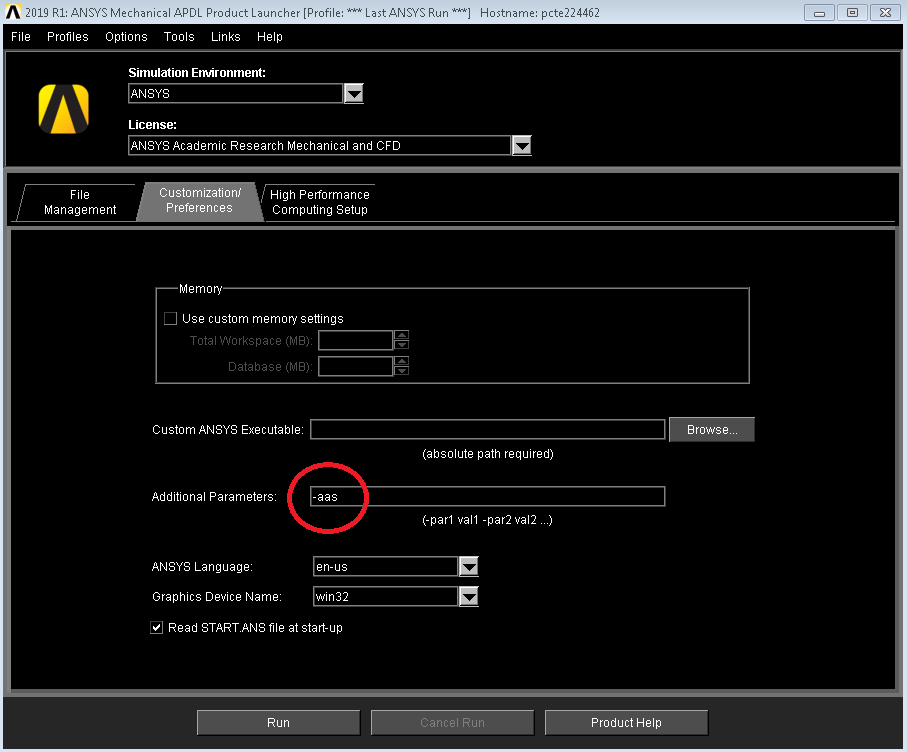
\includegraphics[width=.5\textwidth]{sections/appendices/analysis_in_python/ANSYS_APDL_launching_scheme.png}};
    \end{tikzpicture}
    \caption{ANSYS APDL launching scheme.}
    \label{fig:ansys_apdl_launching_scheme}
\end{figure}

The representative code for Python compilation with ANSYS environment is presented in Table~\ref{table:ansys_python_compilation}. By using the methods .executeCommandToString(), one can simply translate ANSYS APDL scripting commands into a Python language.

\begin{table}[h!]
    \caption{Compilation of Python with ANSYS environment} 
    \vspace{-1em} 
    \fontsize{10}{10}
    \selectfont 
    \renewcommand{\arraystretch}{1}
    \begin{center}
    \begin{tabular}{ ll }  
    \hline  
        from ansys\_corba import CORBA & - imports ANSYS library \\
        os.chdir(directory) & - sets analysis directory\\
        with open('aaS\_MapdlID.txt', 'r') as f: \\ aasMapdlKey = f.read() & - opens APDL analysis \\
        mapdl = CORBA.ORB\_init().string\_to\_object(aasMapdlKey) & - creates mapdl object \\
    \hline
        mapdl.executeCommandToString("/prep7") & - exemplary command \\
     \end{tabular} 
    \end{center}  
     \label{table:ansys_python_compilation} 
 \end{table}


\section{Execution Script in Python}
\label{appendix:execution_script_python}

\renewcommand{\baselinestretch}{0.8} 
\begin{verbatim}
from source.factory.factory import Factory

# creation of analysis directories
json_file_directory = "C:\\skew_quad_analysis"
json_filename = "input.json"
factory = Factory(json_file_directory, json_filename)

######################################################
# DEFINITION OF INITIAL INSTANCES TO RUN THE PROGRAMME
######################################################

ans = factory.get_ansys_class(factory)
mat = factory.get_material_properties_class(factory)
mag = factory.get_magnetic_map_class(factory)
v_quench = factory.get_quench_velocity_class()

#########################
# GENERAL PRE-PROCESSOR #
#########################

# definition of initial magnetic field, 
# initial material properties and coil geometry
preprocessor = factory.get_preprocessor_class(
    mat_props=mat, ansys_commands=ans, factory=factory)
preprocessor.create_ansys_input_variable_file()
preprocessor.define_material_properties(
    magnetic_map=mag.im_short_mag_dict)
preprocessor.define_geometry()
# since geometry is created, Python starts mapping procedure
coil_geo = factory.get_geometry_class(factory)
preprocessor.include_class_geometry_in_class_instance(
    class_geometry=coil_geo)
# input circuit creator
circuit = factory.get_circuit_class(
    ansys_commands=ans, class_geometry=coil_geo, factory=factory)

############################
# INITIAL TIME STEP SOLVER #
############################

# creation of instances necessary to run the solver
ic_temperature = factory.get_initial_temperature_class(
    ansys_commands=ans, factory=factory,
    class_geometry=coil_geo, mat_props=mat)
solver = factory.get_solver_type(
    mat_props=mat, mag_map=mag, 
    ansys_commands=ans, class_geometry=coil_geo,
    circuit=circuit, ic_temperature_class=ic_temperature, 
    factory=factory)
# adjustment of resistive material 
# properties in initially quenched zone
solver.create_ic_temperature_profile()
postprocessor = factory.get_postprocessor_class(
    class_geometry=coil_geo, ansys_commands=ans,
    v_quench=v_quench, solver=solver, factory=factory)
postprocessor.check_quench_state()
postprocessor.plot_quench_state_in_analysis()
preprocessor.adjust_material_properties_in_quenched_zone(
    postprocessor)
solver.end_of_time_step()

ans.enter_solver()
solver.set_circuit_bcs()
solver.set_initial_temperature()
solver.set_time_step_temperature()
solver.set_solver_boundary_conditions()
solver.enter_solver_settings()
solver.set_time_step()
solver.solve()

####################################
# INITIAL TIME STEP POST-PROCESSOR #
####################################
ans.enter_postprocessor()
# write down temperature profile, plot temperature
postprocessor.get_temperature_profile()      
postprocessor.get_current()
postprocessor.check_quench_state_heat_balance()
# estimate resistance in ansys and python, plot resistance
postprocessor.estimate_coil_resistance()     
postprocessor.estimate_quench_velocity()
postprocessor.check_quench_state_quench_velocity()
postprocessor.plot_quench_state_in_analysis()
ans.finish()

ans.enter_preprocessor()
postprocessor.update_magnetic_field()
preprocessor.adjust_material_properties_in_quenched_zone(
    postprocessor)
preprocessor.adjust_material_properties_in_non_quenched_zone(
    postprocessor, circuit)
# QDS verifying the quench state
preprocessor.start_discharge_after_qds_switch(
    circuit, postprocessor)
preprocessor.adjust_nonlinear_inductance(circuit)
solver.end_of_time_step()

############################
# FURTHER TIME STEP SOLVER #
############################
for i in range(2, len(solver.time_step_vector)):
    ans.enter_solver()
    solver.restart_analysis()
    solver.set_time_step()
    solver.set_time_step_temperature()
    solver.solve()

####################################
# FURTHER TIME STEP POST-PROCESSOR #
####################################
    ans.enter_postprocessor()
    # write down temperature profile
    postprocessor.get_temperature_profile()    
    postprocessor.get_current()
    postprocessor.check_quench_state_heat_balance()
    # estimate resistance in ansys and python, plot resistance
    postprocessor.estimate_coil_resistance()  
    postprocessor.estimate_quench_velocity()
    postprocessor.check_quench_state_quench_velocity()
    postprocessor.plot_quench_state_in_analysis()

    ans.enter_preprocessor()
    postprocessor.update_magnetic_field()
    preprocessor.adjust_material_properties_in_quenched_zone(
        postprocessor)
    preprocessor.adjust_material_properties_in_non_quenched_zone(
        postprocessor, circuit)

    # QDS verifying the quench state
    preprocessor.start_discharge_after_qds_switch(
        circuit, postprocessor)
    preprocessor.adjust_nonlinear_inductance(circuit)
    solver.end_of_time_step()

postprocessor.make_gif()
ans.save_analysis()
ans.terminate_analysis()
factory.copy_ansys_analysis_files_to_output_results_directory()
    
\end{verbatim}

\section{Quench Front Position Assignment Algorithm}
\label{appendix:python_nodes_search_algorithm}

\begin{verbatim}
   
class SearchNodes(object):

    @staticmethod
    def search_node(position, coil_length, epsilon=0.000001):
        """
        Uses binary search to find initial quench node
        :param position: initial quench position in meters
        :param coil_length: coil length numpy array; 
                            1st column - node number, 
                            2nd column position in meters
        :param epsilon: searching error as float (optional)
        :return: node number as integer
        """
        
        # check if position is in the coil region
        if position > coil_length[len(coil_length) - 1, 1]:
            raise Exception("ERROR - search_init_node - 
                init. quench position is further than 
                the coil length.")
        elif position < coil_length[0, 1]:
            raise Exception("ERROR - search_init_node - 
                init. quench position is below the start 
                of the coil length.")
        guess_epsilon = None
        left = 0
        right = len(coil_length)-1
        guess = round((left + right)/2)
        
        while abs(coil_length[guess, 1] - position) > epsilon:
        
            if guess == guess_epsilon:
                # compare which border is closer
                if abs(coil_length[right, 1] - position) < \
                abs(coil_length[left, 1] - position):
                    return right+1
                else:
                    return left+1
            if coil_length[guess, 1] < position:
                left = guess
            else:
                right = guess
            guess_epsilon = guess
            guess = round((left + right)/2)

        # counting nodes in ansys starts from 1
        return guess + 1
\end{verbatim}

\section{Quench Detection Algorithm}
\label{appendix:python_quench_detection_algorithm}

\begin{verbatim}
    
    class QuenchDetect(object):

    def __init__(self, class_geometry, npoints, mat_props):
        """
        :param coil_length:
        :param directory: analysis_directory as string
        :param npoints: number of nodes in geometry as integer
        """

        self.mat_props = mat_props
        self.geo = class_geometry
        self.coil_length = self.geo.coil_geometry
        self.npoints = npoints

    def detect_quench(self, input_quench_front_vector, 
                      temperature_profile, magnetic_field_map):
        """
        Main function for quench detection
        :param input_quench_front_vector: 
               list of QuenchFront objects
        :param temperature_profile: 
               file with nodal temperature as string
        :param magnetic_field_map: 
               magnetic field winding map as dictionary
        :return: list of new quench fronts positions in meters
        """
        input_quench_front_vector_sorted = 
            QuenchDetect.sort_input_quench_front_vector(input_quench_front_vector)
        temperature_profile_sliced = 
            QuenchDetect.slice_temperature_profile(
            input_quench_front_vector=input_quench_front_vector_sorted, 
            temperature_profile=temperature_profile)
        temp_profile_windings_sliced = 
            self.slice_temperature_profile_with_respect_to_winding_numbers(
            temperature_profile_sliced)
        temp_profile_sliced_quench_detection = 
            self.find_quenched_nodes(temp_profile_windings_sliced, 
                                     magnetic_field_map)
        new_quenched_fronts_before_rejection = 
            QuenchDetect.find_new_quench_fronts(
            quenched_nodes=temp_profile_sliced_quench_detection)
        new_quench_fronts_list = 
            QuenchDetect.create_new_quench_fronts_list(
            input_quench_front_vector=input_quench_front_vector_sorted, 
            new_quench_fronts=new_quenched_fronts_before_rejection)
        new_quench_fronts_list_without_repetitions = 
            QuenchDetect.find_repetitive_fronts(new_quench_fronts_list)
        new_quench_fronts_sorted = 
            QuenchDetect.define_final_new_quench_fronts(
            fronts_list=new_quench_fronts_list_without_repetitions, 
            new_quench_fronts_nodes=new_quenched_fronts_before_rejection)
        quench_fronts_position = 
            QuenchDetect.search_quench_length(
            coil_length=self.coil_length, 
            new_quench_fronts_nodes=new_quench_fronts_sorted)
        return quench_fronts_position

    @staticmethod
    def sort_input_quench_front_vector(input_quench_front_vector):
        """
        :param input_quench_front_vector: list of QuenchFront objects
        :return: list of QuenchFront objects sorted 
                 from lowest x_down to highest x_down
        """
        return sorted(input_quench_front_vector, 
               key=lambda QuenchFront: QuenchFront.x_down)

    @staticmethod
    def slice_temperature_profile(input_quench_front_vector, temperature_profile):
        """
        :param input_quench_front_vector: list of QuenchFront objects
        :param temperature_profile: temperature profile as numpy array
        :return: list of non-quenched zones as numpy arrays
        """
        node_down_list = []
        for items in input_quench_front_vector:
            node_down_list.append(items.x_down_node)
        node_up_list = []
        for items in input_quench_front_vector:
            node_up_list.append(items.x_up_node)

        sliced_temperature_profile = []
        if len(input_quench_front_vector) != 0:
            for i in range(len(input_quench_front_vector) + 1):
                if i == 0:
                    sliced_temperature_profile.append(
                    temperature_profile[0:(node_down_list[i]-1), :])
                elif i == len(input_quench_front_vector):
                    sliced_temperature_profile.append(
                    temperature_profile[
                    (node_up_list[i-1]):(len(temperature_profile)), :])
                else:
                    sliced_temperature_profile.append(
                    temperature_profile[
                    (node_up_list[i-1]):(node_down_list[i]-1), :])
            print("Number of zones to check for quench is: {}"
            .format(len(sliced_temperature_profile)))
        else:
            sliced_temperature_profile.append(temperature_profile)
        return sliced_temperature_profile

    def slice_temperature_profile_with_respect_to_winding_numbers(
        self, sliced_temp_profile):
        """
        Returns list of dictionaries; each dictionary divides 
        a sliced temperature profile into sub-regions
        with respect to winding number
        :param sliced_temp_profile: 
               list of non-quenched zones 
               (list of nodes) as numpy arrays
        :return: list of dictionaries; 
                 each dictionary assigns node numbers 
                 to different winding number
        """
        sliced_temp_wind_profile_list = []
        for slice_pro in sliced_temp_profile:
            if len(slice_pro) != 0:
                dict_slice = {}
                slice_node = slice_pro[:, 0]
                winding_temp_dict = self.geo.
                retrieve_winding_numbers_and_quenched_nodes(
                    x_down_node=slice_node[0], 
                    x_up_node=slice_node[len(slice_node)-1])
                for key in winding_temp_dict:
                    value = winding_temp_dict[key]
                    temp_profile_winding = slice_pro[
                    np.where(slice_pro[:, 0] >= int(value[0]))]
                    temp_profile_winding = temp_profile_winding[
                    np.where(temp_profile_winding[:, 0] <= int(value[1]))]
                    dict_slice[key] = temp_profile_winding
                sliced_temp_wind_profile_list.append(dict_slice)
        return sliced_temp_wind_profile_list

    def find_quenched_nodes(
        self, sliced_temp_wind_profile_list, magnetic_map_dict):
        """
        Returns list of quenched nodes by counting 
        critical temperature dependent on magnetic field at each winding
        :param sliced_temp_wind_profile_list: list of dictionaries
        :param magnetic_map_dict: magnetic map as dictionary 
                assigning different magnetic field to each winding
        :return: list of newly quenched nodes (list of integers)
        """
        quenched_nodes = []
        for item in sliced_temp_wind_profile_list:
            for key in item:
                array = item[key]
                mag_field = magnetic_map_dict[key]
                critic_temp = self.mat_props.
                    critical_current_density.critical_temperature(
                    magnetic_field=mag_field)
                temporary_quenched_nodes = array[
                    np.where(array[:, 1] >= critic_temp)]
                if len(temporary_quenched_nodes) != 0:
                    quenched_nodes.append(temporary_quenched_nodes)
        return quenched_nodes

    @staticmethod
    def find_new_quench_fronts(quenched_nodes):
        """
        :param quenched_nodes: list quenched 
                                nodes as numpy arrays
        :return: list of lists in each of which 
                 there is lower and upper node of new quench fronts
        """
        new_quench_fronts = []
        for quenched_nodes_sliced_profiles in quenched_nodes:
            x_up_node = 0
            x_down_node = 0
            while x_up_node < len(quenched_nodes_sliced_profiles):
                while x_up_node < len(quenched_nodes_sliced_profiles)-1 
                    and quenched_nodes_sliced_profiles[x_up_node+1][0] - \
                    quenched_nodes_sliced_profiles[x_up_node][0] == 1:
                        x_up_node += 1
                new_quench_fronts.append([
                    int(quenched_nodes_sliced_profiles[x_down_node][0]),
                    int(quenched_nodes_sliced_profiles[x_up_node][0])])
                x_down_node = x_up_node + 1
                x_up_node += 1
        return new_quench_fronts

    @staticmethod
    def create_new_quench_fronts_list(
        input_quench_front_vector, new_quench_fronts):
        """
        :param input_quench_front_vector: 
            list of QuenchFront objects
        :param new_quench_fronts: list of lists 
            in each of which there is lower 
            and upper node of new quench fronts
        :return: list of indices of new quench fronts 
            which are directly neighboring with existing quench fronts
        """
        initial_quench_fronts = []
        for items in input_quench_front_vector:
            initial_quench_fronts.append([items.x_down_node, items.x_up_node])
        fronts_to_delete = []
        for i in range(len(initial_quench_fronts)):
            for j in range(len(new_quench_fronts)):
                if abs(initial_quench_fronts[i][0] - new_quench_fronts[j][1]) == 1:
                    fronts_to_delete.append(j)
        for i in range(len(initial_quench_fronts)):
            for j in range(len(new_quench_fronts)):
                if abs(initial_quench_fronts[i][1] - new_quench_fronts[j][0]) == 1:
                    fronts_to_delete.append(j)
        return fronts_to_delete

    @staticmethod
    def find_repetitive_fronts(duplicate):
        """
        Removes repeating indices in the list of indices
        :param duplicate: list of indices of new quench 
            fronts which are directly neighboring 
            with existing quench fronts
        :return: list of indices of new quench 
            fronts to delete without repetitions
        """
        final_list = []
        for num in duplicate:
            if num not in final_list:
                final_list.append(num)
        return final_list

    @staticmethod
    def define_final_new_quench_fronts(fronts_list, new_quench_fronts_nodes):
        """
        :param fronts_list: list of indices of new 
            quench fronts to delete without repetitions
        :param new_quench_fronts_nodes: list of lists in each 
            of which there is lower and upper node of new quench fronts
        :return: list of new quench fronts without the ones 
            neighboring with the existing ones
        """
        fronts_list.sort()
        fronts_list.reverse()
        print("Number of quench fronts faster 
            than current quench fronts: {}".format(len(fronts_list)))
        for i in range(len(fronts_list)):
            new_quench_fronts_nodes.remove(
            new_quench_fronts_nodes[fronts_list[i]])
        print("New quench fronts [nodes]: {}".format(new_quench_fronts_nodes))
        return new_quench_fronts_nodes

    @staticmethod
    def search_quench_length(coil_length, new_quench_fronts_nodes):
        """
        :param coil_length: length of coil for each node as numpy array
        :param new_quench_fronts_nodes: list of final new quench fronts
        :return: list of position of new quench fronts
        """
        new_quench_node_list = new_quench_fronts_nodes
        new_quench_length_list = []
        for sublist in new_quench_node_list:
            new_x_down = coil_length[sublist[0]-1][1]
            new_x_up = coil_length[sublist[1]-1][1]
            print("New quench zone; x_down= {}, 
                x_up= {}".format(new_x_down, new_x_up))
            new_quench_length_list.append([new_x_down, new_x_up])
        return new_quench_length_list

\end{verbatim}

\end{appendices}

\clearpage
\bibliographystyle{IEEEtran}
\bibliography{./bib/article}

\end{document}
